%  ========================================================================
%  Copyright (c) 1995-2012 The University of Washington
%
%  Licensed under the Apache License, Version 2.0 (the "License");
%  you may not use this file except in compliance with the License.
%  You may obtain a copy of the License at
%
%      http://www.apache.org/licenses/LICENSE-2.0
%
%  Unless required by applicable law or agreed to in writing, software
%  distributed under the License is distributed on an "AS IS" BASIS,
%  WITHOUT WARRANTIES OR CONDITIONS OF ANY KIND, either express or implied.
%  See the License for the specific language governing permissions and
%  limitations under the License.
%  ========================================================================
%

% Documentation for UW thesis document style for LaTeX
% by Jim Fox
% fox@washington.edu
%
%    Revised for version 2012/06/19 of uwthesis.cls
%
%    This document is contained in a single file ONLY because
%    I wanted to be able to distribute it easily.  A real thesis ought
%    to be contained on many files (e.g., one for each chapter, at least).
%
%    To help you identify the files and sections in this large file
%    I use the string '==========' to identify new files.
%
%    To help you ignore the unusual things I do with this sample document
%    I try to use the notation
%       
%    % --- sample stuff only -----
%    special stuff for my document, but you don't need it in your thesis
%    % --- end-of-sample-stuff ---


%    Printed in twoside style now that that's allowed
%
 
\documentclass [11pt, twoside] {uwthesis}[2012/06/19]
%\usepackage{draftcopy}
 
\usepackage{type1cm}
\usepackage{eso-pic}
\usepackage{color}
\usepackage{listings}
\usepackage{mdwlist}
\usepackage{MnSymbol}

\usepackage{hyperref}
\usepackage{fancyhdr}
\usepackage{setspace}

\setlength{\headheight}{14pt}

\usepackage{nicefrac}
\usepackage{xcolor}


\usepackage{pdfpages}

%\usepackage[table]{xcolor}

%% Uncomment below to add the DRAFT to the page
 %\makeatletter
 %\AddToShipoutPicture{%
 %           \setlength{\@tempdimb}{.5\paperwidth}%
 %           \setlength{\@tempdimc}{.5\paperheight}%
 %           \setlength{\unitlength}{1pt}%
 %           \put(\strip@pt\@tempdimb,\strip@pt\@tempdimc){%
 %       \makebox(0,0){\rotatebox{45}{\textcolor[gray]{0.90}%
 %       {\fontsize{6cm}{6cm}\selectfont{DRAFT}}}}%
 %           }%
 %}
%% Uncomment above... ^

%\makeatletter % Reference list option change
%\renewcommand\@biblabel[1]{} % from [1] to 1.
%\makeatother %

\makeatother

%
% The following line would print the thesis in a postscript font 
%\usepackage[style=alphabetic,natbib=true]{biblatex}

 \usepackage[square]{natbib}
 \def\bibpreamble{\protect\addcontentsline{toc}{chapter}{Bibliography}}
%
\setcounter{tocdepth}{3}  % Print the chapter and sections to the toc
\setcounter{secnumdepth}{5} 

\usepackage{graphicx}
\usepackage{floatrow}
\floatsetup[table]{font=sf}

%\usepackage{caption}
%\usepackage{subcaption}

% will apply to all captions
\usepackage[font={small,singlespacing}]{caption} 
% will apply to all subcaptions
\usepackage[font={small,stretch=1,sf},singlelinecheck=off,justification=raggedright]{subcaption}

%\usepackage{subfig}
\usepackage{rotating}

\usepackage{booktabs,tabularx}
\usepackage{multirow}
% ==========   Local defs and mods
%

% --- sample stuff only -----
% These format the sample code in this document

\usepackage{alltt}  % 
\newenvironment{demo}
  {\begin{alltt}\leftskip3em
     \def\\{\ttfamily\char`\\}%
     \def\{{\ttfamily\char`\{}%
     \def\}{\ttfamily\char`\}}}
  {\end{alltt}}
 
% metafont font.  If logo not available, use the second form
%
% \font\mffont=logosl10 scaled\magstep1
\let\mffont=\sf
\usepackage{palatino}
% --- end-of-sample-stuff ---
 


\begin{document}
 
% ==========   Preliminary pages
%
% ( revised 2012 for electronic submission )
%

\prelimpages
 
%
% ----- copyright and title pages
%
\Title{Approaches to Food Journaling on Mobile Devices}
\Author{Adrienne Hope Andrew}
\Year{2012}
\Program{Computer Science and Engineering}

\Chair{Name of Chairperson}{Title of Chair}{Department of Chair}
\Signature{James Fogarty}
\Signature{Julie Kientz}
\Signature{Wanda Pratt}

%\copyrightpage

% \titlepage  

% --- sample stuff only -----
% unusual footnote not found in a real thesis
% You just use the \titlepage as commented out above

{\Degreetext{A dissertation\\
  submitted in partial fulfillment of the\\ requirements for the degree of}
 \def\thefootnote{\fnsymbol{footnote}}
 \let\footnoterule\relax
 \titlepage
 }
\setcounter{footnote}{0}

% --- end-of-sample-stuff ---
 
%
% ----- signature and quoteslip are gone
%

%
% ----- abstract
%


\setcounter{page}{-1}
\abstract{%
A healthy diet has the power to both prevent and heal disease, and the
high rates of lifestyle- and diet-related disease in America indicates the
need for tools to help improve diet. Self-monitoring one's food intake is
considered key to improve one's eating behaviors. The consumer demand for
health and wellness tools, especially on personal, always-with-us mobile
devices, shows both the interest on behalf of users and the resources on
behalf of creators. However, few individuals are able to sustain the
self-monitoring practice for an appropriate length of time, and many
people complain about the poor experience they have had using food
journals.

I examine self-monitoring of food intake using mobile phones. Overall, I
characterize problems people encounter using a traditional
database-oriented food journal, provide motivation for rethinking this
approach, and describe a series of studies that investigate the use of a
reduced-detail self-monitoring tool for dietary intake.
}
 
%
% ----- contents & etc.
%
\tableofcontents
\listoffigures
\listoftables  
 
%
% ----- glossary 
%

\chapter*{Glossary}      % starred form omits the `chapter x'
\addcontentsline{toc}{chapter}{Glossary}
\thispagestyle{plain}
%
\begin{glossary}
\item[diary] The artifact. 
\item[journaling] The process of creating a food entry. 
\item[self-monitoring] The process of monitoring, more abstract. 
\item[food entry] An entry in a diary that represents a food. 
\item[dietary intake]

\item[table] information placed in a columnar arrangement.
\item[thesis] either a master's thesis or a doctoral dissertation.
This document also refers to itself as a thesis, although it
really is not one.
 
\end{glossary}

 
%
% ----- acknowledgments
%
\acknowledgments{% \vskip2pc
  % {\narrower\noindent
  The author wishes to express sincere appreciation to
  University of Washington, where he has had the opportunity
  to work with the \TeX\ formatting system,
  and to the author of \TeX, Donald Knuth, {\it il miglior fabbro}.
  % \par}
}

%
% ----- dedication
%
\dedication{\begin{center}to Mazzy Star and Alec Ivan.\end{center}}

%
% end of the preliminary pages
 
 
 
%
% ==========      Text pages
%

\textpages


% ========== Intro
 \chapter {Introduction}

This dissertation explores how people use mobile phone food diaries to self-monitor their dietary intake. In this chapter, I identify some factors that influence what people eat; provide background on how what people eat impacts their health; and introduce how technologies that influence dietary intake can impact society. 

\section{Introduction}
Globally, the incidence of lifestyle diseases such as obesity, diabetes and cardiovascular disease are increasing. One-third (34\%) of adults were overweight or obese in 2008 \citep{kimokoti_diet_2011}. The prevalence of diabetes for all age groups, worldwide, is expected to rise from 6.4\% in 2010 to 7.7\% (439 million people) in 2030 \citep{Shaw20104}. Researchers believe this to be an underestimate. Cardiovascular disease (CVD) is the number one cause of death globally. 17.3 million people died from CVDs in 2008, accounting for about 30\% of worldwide deaths \citep{WHO_CVD_2011}. Additionally, it is estimated that at least 50\% of cancers are preventable by encouraging healthy behaviors and discouraging unhealthy practices. Cancer accounted for 7.6 million deaths in 2008. The estimated number of new cancer cases in 2030 is 21.4 million, with 13.2 million deaths \citep{american_cancer_society_global_2011}. 

Overweight and obesity are major risk factors for cardiovascular disease (CVD), Type 2 diabetes mellitus, and certain forms of cancer \citep{guh_incidence_2009} \citep{calle_overweight_2004}. 

Lifestyle diseases are so named because they are associated with how a person lives and the choices they make. Lifestyle choices include what and how much to eat, physical activity levels, alcohol consumption, tobacco use, sleep habits, and stress management. Obesity, diabetes, cardiovascular disease and some cancers are all considered lifestyle disease. Generally, researchers believe that lifestyle choices not only impact the incidence or likelihood of developing these diseases, but can also help to treat or reduce the impact of these diseases. 

Researchers believe that a primary cause of obesity is an imbalance of energy intake and expenditure: People eat too many calories while not burning enough calories. While obesity is a risk factor for CVD, diabetes and cancer, it is believed that these diseases are also impacted by what people eat. In addition to balancing caloric intake, the American Heart Association recommendations for preventing cardiovascular disease includes consuming a diet rich in fruits and vegetables, choosing whole grain--high fiber foods, limiting saturated fat intake, and reducing consumption of added sugars and alcohol \citep{Lichtenstein2006}. Similar recommendations are made for preventing diabetes \citep{Hu2001, Thomas2012}. 

Traditionally, researchers believe what people eat is due to biological, psychological, behavioral and social factors. \citet{furst_food_1996} found that food choice included ``ideals, personal factors, resources, social contexts and the food context''. Food choice incorporates ``value negotiations and behavioral strategies''. Values reflect taste and texture of foods, cost, health and nutritional concerns, availability, and social context. 

More recently, researchers believe that the built environment also impacts what people choose to eat. Built environment includes urban design, land use, availability of public transportation, and activity options in an area \citep{Booth2005}. This also reflects the number of fast food restaurants, convenience stores, bars, food distribution programs with high-fat foods, and concentrated media marketing. Poorer neighborhoods have fewer supermarkets and more places to consume alcohol than wealthier neighborhoods \citep{Morland2002}. This impacts the availability of healthy food. 

The food industry plays a role in the over consumption of food in America. Serving sizes have increased over time \citep{Nielsen2003}: Commercial serving sizes are at least twice the size and as much as eight times the size of standard serving sizes defined by the USDA and FDA \citep{Young2003, Nielsen2003}. Servings provided by fast--food chains are now two to five times original sizes \citep{Young2003}. Calories provided by the US food supply increased from 3200 in the 1970s to 3900 in 1990s \citep{Nestle2002}. When more food is available, manufacturers need to compete harder for their share of consumer dollars. The increased marketing encourages people to eat more. 

However, the external environment takes a long time and many resources to change. Providing support for individuals to insulate themselves from the environment and change their own behavior could have a more immediate impact.  \citep{Hill2006}
Research indicates that self-monitoring of dietary intake does help change behavior \citep{burke_experiences_2009,burke_self-monitoring_2005, burke_self-monitoring_2011}. 

Many people are not well aware of what, why or how much they eat.   While people tend to underestimate energy intake \citep{Schoeller199518,Black1991583,Livingstone1990}, in general they are unsure of how many calories they burn in physical activity (energy expenditure) \citep{Prince2008}. This tendency results in an unawareness of the actual overall balance of caloric intake and expenditure, which results in weight gain. 

People underestimate energy intake for a variety of reasons, including a lack of awareness of how many calories are in food \citep{Zegman1984}; what an appropriate serving size is \citep{Young2009, beasley_accuracy_2005}; erroneous estimates of how much of a food has been eaten \citep{beasley_accuracy_2005}; and neglecting to consider calorie dense condiments or additions to a food \citep{Zegman1984}. This effect is magnified when a person does not document what they eat as soon as they eat it, and time passes between consumption and recording \citep{Baranowski1994}. Additionally, although reflecting on food intake in the past (e.g., earlier in the day) may help raise an individual's awareness of calories in given foods, it does not enable them to make good decisions in the moment. Timely access to calorie data could help people not only capture and understand how many calories they have already consumed for the day, but also make better decisions going forward. 

People also underestimate the number of calories they burn over time. An estimate of energy expenditure by a person in a given time period is the sum of three items: the base metabolism for that individual (how many calories their body consumes for basic bodily function), the amount and intensity of intentional exercise (e.g., going for a run) and the amount and intensity of unintentional exercise (e.g., how much walking versus sitting a person does). It is relatively easy for people to measure their intentional exercise, as it's usually well-defined. However, humans tend to vastly overestimate their unintentional exercise \citep{Duncan2001}. Readily available technology such as wearable sensors can keep track of general activity for an individual, allowing them to more closely track energy expenditure over time. 

The field of persuasive technology aims to use computers and technology to persuade or nudge people to change their behavior, in a way that they want to change \citep{Fogg2002}. 

Ubiquitous mobile devices such as smartphones have been considered ideal platforms for administering behavior change programs, especially around eating behaviors. They enable kairos-- the availability of relevant information and decision support at the time of need. That is, these devices allow people to self-monitor what they eat by providing a means to capture what has already been eaten, and looking up caloric values for prospective foods. This allows people to make an informed decision. However, formal research and informal feedback indicates that people have difficulties adhering to the use of mobile-phone food diaries for extended periods of time. 

This dissertation focuses on the use of mobile technologies to support people in becoming more aware of their nutrition behaviors and make better choices. 

\section{Contributions}
In this dissertation I offer four contributions toward understanding and helping people use technology to monitor and change their dietary behaviors. The first is the BALANCE project, which provided timely feedback of daily energy balance by using sensors to automatically detect physical activity and calculate energy expenditure. The sensing device was wirelessly connected to a mobile phone. Users entered their food intake into a food diary on the mobile phone. A glanceable display provided a visualization of the current and target energy intake and expenditure. My role was to design, build and evaluate the mobile phone food diary and visualization. This allowed me to examine and characterize challenges with database-oriented food diaries.  

BALANCE inspired contribution two, the evaluation of food diary prototypes with a focus on diet quality and goal tending. Feedback from participants using the BALANCE project revealed user dissatisfaction with using a database to look up what they were eating. This led me to explore ways to monitor food intake without using a database. I took a pattern-based approach to self-monitoring, where users would monitor an overall pattern of food consumption rather than a detailed list. I used a theory-driven, user-centered design process to generate mobile-phone food diary prototypes. I evaluated the usability and potential utility of the prototypes in a lab setting to generate design principles and guidelines for designing a dietary-pattern-based mobile phone food diary. 

For contribution three, I used the design principles and guidelines from the lab studies to design and build a dietary-pattern-based mobile phone food diary. I used an iterative approach, beginning with sketches and paper prototypes, evaluating wireframes, and finally interactive prototypes. This contribution includes a design rationale for each feature of the final pattern-oriented nutrition diary prototype. 

Finally, my fourth contribution is an evaluation of the use of the pattern-oriented nutrition diary by people in their daily lives. The evaluation provides insight into how the design of self-monitoring tools impact how people think about what they eat. 

\section{Roadmap}
Chapter \ref{cha:relatedWork} describes background in psychology and epidemiology that focuses on behavior change and how to support it. It also reviews related work and how it differs from the work presented in this dissertation.  Chapter \ref{cha:cont1} describes the BALANCE project, which explored one approach to supporting people in self-monitoring food intake and physical activity. Chapter \ref{cha:cont2} describes background and a study that shows that there could be benefit in designing a food diary that requires less input and thinking. Chapter \ref{cha:cont3} describes the design of POND, which is a food diary based on the results of the study in Chapter \ref{cha:cont2}. Chapter \ref{cha:cont4} evaluates the POND food diary. Chapter \ref{cha:futureWork} concludes this dissertation with a summary and discussion of future work. 

\chapter{Background}
\label{cha:background}
This chapter covers background material that informs this dissertation. This primarily consists of the psychological and cognitive theories of behavior, learning and change that relate to self-monitoring. These theories inform the design of interventions to change behavior, either in general or specifically for nutrition behaviors. This background will highlight the role and importance of self-monitoring as a tool for nutrition behavior change. Included in this background is persuasive technology, which uses the aforementioned theories to define strategies and tactics of employing technology to nudge behavior. 

 This chapter will introduce the various theories and related concepts that impact the design and evaluation of the self-monitoring tools presented in this dissertation. 

\section{Introduction}



\section{Behavior Change}
In this section, I review some relevant theories in regards to behavior change. 

\subsection{Theory of Planned Behavior} 
The Theory of Planned Behavior (TPB) is a model of individual behavior that assumes a person is a rational actor. It builds off the Theory of Reasoned Action (TRA). TRA states that a person's behavior is determined by behavioral intention. Behavioral intention depends on attitude (individual beliefs about a behavior) and a subjective norm. The subjective norm stems from the individual's normative beliefs, which is defined as whether influential parties approve or disapprove of the behavior in question. 

This is embodied in the real world by:
* Calculating attitude:
	* measuring likelihood that a target behavior will result in a specific outcome. 
	* Evaluating the [attractiveness] of an outcome (whether the outcome is good or bad). 
	* combine the above two items for each potential outcome of a behavior. 
	* combine all the combinations to determine the individual's attitude toward that change. 
* Calculating normative beliefs:
	* For each identified referent (parent, doctor, peer...):
		* The individual rates how the referent feels about the individual performing the target behavior. 
		* The individual rates how much influence that referent has on their behavior (ie, ``I agree that I want to do what my doctor thinks I should do''). 
		* combine the above two items. 
	* Combine the results for each referent. 

The Theory of Planned Behavior (TPB) extends TRA by including a component of volitional control. Volitional control captures the individual's ability to exercise control over the target behavior. Volitional control is included in the model by perceived behavioral control. If the individual perceives a great amount of behavioral control, then motivation (as characterized by TRA) drives the individual's performance of the target behavior. If the individual perceives little control over their ability to execute the target behavior, the individual expends less effort in pursuit of the target behavior. Perceived control depends on control beliefs and perceived power of each belief. 
 
\subsection{Enabling change: Social Cognitive Theory}
Social Cognitive Theory \citep{bandura_health_2004, bandura_self-efficacy:_1977} posits that a person�s behavior, environment and inner qualities all contribute to how a person functions. This theory has been applied to understanding how people learn, how social environments impact what people do, and how people regulate their own behavior. A key component in this theory is self-efficacy, which is summarized as a belief in one�s abilities.

Self-efficacy is traditionally measured by self-report. To develop self-efficacy measurements for a particular domain, researchers use open-ended approaches to identify common challenges and barriers to the problem. They then develop a series of statements of the form ``How confident are you that you can [achieve goal] even though [challenge]?'' with a 4-unit response scale ranging from ``Cannot do it'' to ``Highly certain can do''. An example of a statement is ``How confident are you that you can stick to a healthy eating plan after a long, tiring day at work?''

Research shows self-efficacy measures based on self-report indicate adherence to strategies to change behavior \citep{nothwehr_self-efficacy_2008}. While short-term studies cannot prove behavior change, self-efficacy measures provides valuable feedback about whether an intervention is supporting adherence to behavior change strategies, and indicate whether participants complete the study with an intention to continue.

This is an important feature for PI researchers: we are familiar with a domain and common challenges, so can build the scales easily; we usually use short-term studies to indicate long-term impact; and properly designed scales can help us to discover where a PI tool breaks down.

\subsection{The process of change: Transtheoretical Model}
The transtheoretical model (TTM) \citep{prochaska_transtheoretical_1997} reflects that people are in varying stages of change in relation to a given behavior. It arises from study of a theoretical intervention therapies, such as psychoanalysis, gestalt, and cognitive therapies. Across all these theories, Prochaska et al determined that intervention therapies had no time construct. He interviewed people who were not familiar with intervention therapies but had successfully changed a key behavior. He found that change was a process that unfolded over time. This process could be broken into stages, each with certain characteristics. Further, constructs from some theories were applicable in some stages of change, while a seemingly contradictory theoretical construct was appropriate for a different stage of change. A key finding from the TTM inquiry is that no single theory can fully describe and account for the complexities of behavior change. 

The stages include precontemplation, contemplation, preparation, action, and maintenance. A person in the stage of precontemplation does not intend to take action around the target behavior within the next six months. That person moves to contemplation when they intend to take action within the next six mohts, and then into preparation when they intend to take action within thirty days. People in the preparation stage usually have taken some steps toward the change. Action reflects that the person has engaged in the new behavior for less than six month. Finally, maintenance is having continued the new behavior for more than six months. 

Two constructs impact progression from one stage to the next: decisional balance and self-efficacy. Decisional balance is a comparison of the benefits of changing to the costs of changing. To move from the preparation to the action stage, the benefits need to increase by one standard deviation, or the costs need to decrease by half a standard deviation. That is, the person needs to either identify many more benefits to changing, or reduce the impact of a few barriers. Self-efficacy is a measure of how confident an individual is about their ability to continue the target behavior in challenging situations. 

Understanding the TTM is important for designing behavior change interventions because different theoretical constructs and processes apply to different stages of change. For individuals in precontemplation, consciousness raising and environmental reevaluation are key processes. These processes focus on strategies that target education of the individual, or changing how they view themselves in relation to the target behavior. In the action stage, processes such as counterconditioning and helping relationships support continuation of the target behavior. Counterconditioning focuses on how to replace unhealthy behaviors with target behaviors. Helping relationships includes building relationships that support the individual in the change. 



\subsection{Supporting change: Goal setting and tending}
Here I talk about Locke and Latham \citep{locke_building_2002} and Consolvo and Landay \citep{consolvo_goal-setting_2009}. Goal theory. How to define goals. How to support progress toward goals. 

\subsection{Self-Monitoring and Change}

First, I'll talk about what self-monitoring of dietary intake is, and what is involved. Self-monitoring of dietary intake is the process that an individual uses to keep track of what they eat. The self-monitoring process is impacted by both the tool or instrument used for self-monitoring and the individual doing the self-monitoring. In regards to the individual, the process of self-monitoring involves cognitive processes, and the ability or willingness to continue self-monitoring involves individual goals, motivation, and resources.   The design of the tool impacts the process by clarifying (communicating? reminding?) goals as well as responding to individual motivation and resources. 


Research consistently supports that self-monitoring helps to mediate behavior change. Indeed, \citet{kanfer_self-monitoring:_1970} states ``self-observation is an initial step to self-directed behavior change''. Much research in this area falls outside the scope of this chapter, but in the domain of weight-loss, people who adhere to consistent self-monitoring of dietary intake lose more weight and have better indicators of related behaviors. Burke et al and the PREFER trial. WHI. \citep{greaves_systematic_2011}

It is unclear how self-monitoring impacts behavior change, or what mediates the process of self-monitoring. This is primarily due to limitations in the ability to evaluate the self-monitoring process. \citep{Baranowski1994, kanfer_self-monitoring:_1970, burke_self-monitoring_2005, glanz_improving_2006}. 

Later in this chapter I further explore how electronic self-monitoring tools for dietary intake are evaluated. 

\subsection{Self-Monitoring for Health}
Self-monitoring has been key to supporting lifestyle behavior changes necessary for treating cardiovascular disease, diabetes, cancer, and renal disease. 

Electronic self-monitoring has advantages over pencil and paper self-monitoring. 

Certain lifestyle behaviors can help to prevent disease as well as treat it. 

Since many of the behavior changes relate to nutrition and dietary intake, much research focuses on this. However, nutrition literature demonstrates that brief monitoring of the behaviors can still be effective. The technology domain has not put much emphasis on investigating brief monitoring instruments. 

Self-monitoring can help people make the behavior changes that prevent disease. 

The cognitive processes involved in the recall of food have been described in children as \citep{Baranowski1994}:
�    Attention
�    Perception
�    Organisation
�    Retention
�    Retrieval
�    Response formulation
People need to attend to the food that they are eating, at the time they eat it, in order to perceive it. The food information then needs to be organized and stored for retention. Then, the food information needs to be retrieved, and formulated into a response or action (e.g. creating a record). 

\subsection{Technology and Behavior Change (Persuasive Technology)}
In this section, talk about the body of work that has looked at how to use technology to support behavior change. Persuasive technology \citep{Fogg2002} and theory-driven technology \citep{consolvo_theory-driven_2009}. 

\section{Approaches to Changing Nutrition Behaviors}
Here I describe some standard approaches and theories nutritionists use to inform behaviors change to provide as background for reference later in this dissertation. It is not an exhaustive list. 

\subsection{Motivational Interviewing}
Motivational interviewing (MI) \citep{miller_motivational_2002, Miller2002} is a process practitioners use to identify what areas of change an individual is ready for. It is a technique employing goal setting, feedback mechanisms, and self-monitoring. There are three key elements: collaboration rather than confrontation; evoking ideas rather than imposing ideas; and autonomy rather than authority. In addition are four principles to follow: express empathy, support self-efficacy, roll with resistance, and ``develop discrepancy'' (or identify cognitive dissonance). 

MI has a strong record of impact for many types of behavior change \citep{Rubak2005}. It is particularly effective and well respected in the area of nutrition behavior changes \citep{abraham_taxonomy_2008, michie_effective_2009, greaves_systematic_2011}. 

\subsection{CBT Programs}
Cognitive-Behavioral Training (CBT) teaches people how to change the way they think about their nutrition behaviors to support them in the change. 

\subsection{Other techniques}
Other common themes in the research is regular group meetings, personalized feedback, nutritional education. 





\section{Summary}In this section, I reviewed relevant background information for this dissertation, including behavior change theories, traditional approaches specifically for supporting nutrition behavior change, and the important role of  self monitoring. I provided some overviews of how self-monitoring has been studied both from a technology development perspective, and how nutritionists evaluate self-monitoring of dietary intake from a utility perspective. I also provided a short overview of projects related to those discussed in this dissertation. 

% ========== Chapter 1
 



\chapter {BALANCE}
\label{cha:cont1}
In this chapter, I describe my contributions to the BALANCE project. 

\section{Introduction}

The bioengineering approaches for lifestyle activity
and nutrition continuous engagement (BALANCE) project was a multi-year, interdisciplinary project with the goal of designing, building, and evaluating a mobile-phone based application to help people overcome these challenges of tracking their overall balance of energy intake and expenditure. It combines a wearable device that calculates caloric expenditure with a mobile phone that includes a food diary to track caloric intake. The software also includes a visualization that reports the real-time energy balance for the day. The wearable device is built using the multi-sensor board (MSB) \citep{lester_validated_2009}. The MSB contains an accelerometer, now standard in mobile phones, as well as other sensors that aide in physical activity detection.  

The software consists of three main components: a ``fuel gauge'' visualization that reflects the current caloric balance; a food diary; and a physical activity diary. The food diary requires users to enter the details of what they eat, while the physical activity diary accepts input from the external MSB device that calculates most calories burned from physical activity (the exception being water or high-impact sports, which need to be manually entered).
 
\subsection{Project Overview}
Many people were involved in this multi-phase project. The project included brainstorming designs for and evaluation of the fuel-gauge visualization; running a paper prototype evaluation of the software based on specified need, goals and reviews of similar tools; building an initial prototype on a feature phone platform; validating the algorithms on the MSB for calculating calorie expenditure; and executing an iterative design and implementation process of the application on a smartphone. Finally, we combined the smartphone software and MSB validated the system overall. My primary contribution to this project was the design and implementation of the smartphone software. The rest of this chapter describes the process and final product in further detail. 

Multiple documents describe contributions to the BALANCE project. Tamara Denning contributed to the initial design and paper prototype evaluations \citep{denning_balance:_2009}. Deonna Hughes designed, conducted, and analyzed the focus groups and prototype iterations \citep{hughes_balance:_2009}. She looked at two metrics for improvement from iteration to iteration. The first was the result of standardized usability questionnaires; the other was the time between when participants ate a food and when they entered it in the diary. Neither metric showed significant improvement in the prototype over 5 iterations. I discuss this in further detail later in this chapter. Jonathan Lester designed and evaluated the calorie expenditure algorithms \citep{lester_validated_2009}, employing a gold-standard oxygen-consumption evaluation methodology. Algorithms using the MSB sensor data were 89.54\% (+/- 7.25\%) accurate in the lab and 79.8\% (+/- 9.48\%) in the field.  Heather Snively designed and conducted the overall system validation \citep{snively_balance_2010}. Participants used the entire system for 4 days, tracking their food intake on days 1, 3, and 4. On day 2 participants provided a 24-hr recall of what they ate on day 1, which was compared to entries in the food diary on the first day. The average percent calorie difference between the mobile phone food diary and the 24-hr recall was 9 +/- 18\%.  

\section{Fuel-Gauge Visualization}
The goal of the BALANCE project was to combine a food diary to collect information about energy intake, a physical activity component (diary + MSB) to collect energy expenditure information, and the fuel gauge visualization to show the current energy balance throughout the day. The heart of the system was a unifying user interface on a mobile phone. 

The first investigation focused on the fuel-gauge visualization. The visualization needed to provide the current overall energy balance, but it was unclear what other information would be necessary or relevant. Additionally, the visualization needed to be understandable at a glance, provide more meaning upon reflection, and work within the constraints of the target device in terms of size and resolution. One concern was the level of abstraction: whether the visualization depicts a concrete, physical world phenomena or a more mathematically-oriented graph view. In this section, I describe a lab-based paper prototype user study to collect feedback on a wide range of potential visualizations. Results informed the design decisions for the BALANCE prototypes. 

\subsection{Participants}
12 participants (10 female and 2 male) were recruited from a university community. Ages ranged from 18-50, with a majority (8) in the 30-40 year age range. 

\subsection{Procedure}
After providing written informed consent, participants completed a survey collecting basic demographic information. Participants rated the desirability of given features for food and exercise applications on a mobile phone, then discussed what they had eaten that day (or the previous day, depending on time of interview), including context (what they ate, how much, where, when, and how much that meal varies for them). 

Next, participants were shown the different visualizations. Each visualization depicted a different situation: early in the day, before any food is entered or calories expended; the end of the day, when more than the day's goal had been consumed and expended; and two points in between. Figure \ref{fig:viz1series} shows one of the visualization series. 


\begin{figure}[tbh]
	\centering
	\begin{subfigure}[t]{1.25in}
		\centering
		\setlength\fboxsep{0pt}
\setlength\fboxrule{0.5pt}
\fbox{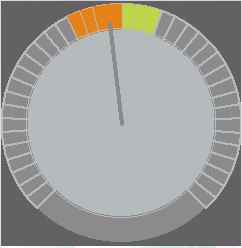
\includegraphics[width=1.25in]{./images/cont1/Viz_1_1}}
		\caption{Shows a day with a small breakfast early in the day. }\label{fig:viz1_1}
	\end{subfigure}
\quad
	\begin{subfigure}[t]{1.25in}
		\centering
		\setlength\fboxsep{0pt}
\setlength\fboxrule{0.5pt}
\fbox{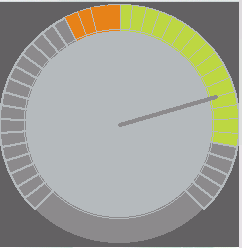
\includegraphics[width=1.25in]{./images/cont1/Viz_1_2}}
		\caption{Shows a day when the user ate a large breakfast. }\label{fig:viz1_2}
	\end{subfigure}
\quad
	\begin{subfigure}[t]{1.25in}
		\centering
		\setlength\fboxsep{0pt}
\setlength\fboxrule{0.5pt}
\fbox{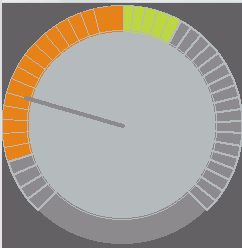
\includegraphics[width=1.25in]{./images/cont1/Viz_1_3}}
		\caption{Represents a day with more exercise early in the day, and some food eaten.}\label{fig:viz1_3}
	\end{subfigure}
\quad
	\begin{subfigure}[t]{1.25in}
		\centering
		\setlength\fboxsep{0pt}
\setlength\fboxrule{0.5pt}
\fbox{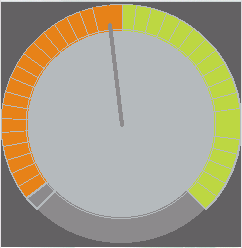
\includegraphics[width=1.25in]{./images/cont1/Viz_1_4}}
		\caption{An end-of-day state, near balance. Both targets are almost met. }\label{fig:viz1_4}
	\end{subfigure}
\quad
	\begin{subfigure}[t]{1.25in}
		\centering
		\setlength\fboxsep{0pt}
\setlength\fboxrule{0.5pt}
\fbox{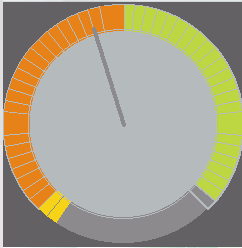
\includegraphics[width=1.25in]{./images/cont1/Viz_1_10}}
		\caption{A near-balance, end-of-day state. Exercise target was surpassed, and food intake was not yet met.}\label{fig:viz1_5}
	\end{subfigure}
\quad
	\begin{subfigure}[t]{1.25in}
		\centering
		\setlength\fboxsep{0pt}
\setlength\fboxrule{0.5pt}
\fbox{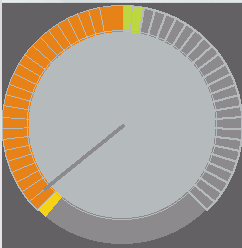
\includegraphics[width=1.25in]{./images/cont1/Viz_1_12}}
		\caption{Lots of exercise, little food eaten.}\label{fig:viz1_6}
	\end{subfigure}

	\caption{Visualizations with various energy intake and expenditure values. }\label{fig:viz1series}
\end{figure}

\begin{figure}

\end{figure}

There were two categories: graphs (two total) and visualizations (five total). Participants were asked to rank their preferred visualizations within each category and offer comments. 

\subsection{Instruments}
The team brainstormed seven candidate visualizations. The features of different visualization concepts included abstract versus concrete metaphors; a single balance indicator (energy balance is more intake or more expenditure); the amount of both energy intake and expenditure as well as overview; how each amount and the balance changes over time; and whether to include an affective component. Previous work investigates the value of having abstract versus concrete representations \citep{Kerren2007}, so we aimed for a wide range at this point in the design process. 

We adopted an overall simplifying construct for calorie counting called ``CHIPs'': counting hundreds impact point (\citep{beresford_worksite_2007}). A CHIP is simply a unit of 100 calories. Experts involved in the project noted previous success with this simplification. In their previous experience, participants in a workplace wellness program found the CHIP simplification easier to count and keep track of larger increments (smaller numbers). In the BALANCE software, all calorie counts are reported in CHIPs, both for intake and expenditure.  

The main goal of the visualization is to depict the current energy balance of intake and expenditure. Other pieces of information that could be helpful included: 
\begin{enumerate*}
\item Goal calorie expenditure and intake for a current day;
\item Progress toward that goal/target over the course of the day; and
\item Whether or how much the user was over the intake or expenditure goal for the day. 
\end{enumerate*}

Mobile phone displays vary greatly in their capabilities, specifically in size and resolution. We used Python for S60 to prototype the visualizations on the target mobile phone, saved them as screenshots, then printed them on paper. This allowed us to present a psuedo-realistic rendering of the visualizations to users. The study artifacts needed to reflect the detail of the visualization within the constraints of the display, as well as the early design stage. Presenting the visualizations on the actual mobile device could raise user
 expectations of the visualization, while paper prototypes and screenshots help to restrain user expectations appropriately. The visualizations were deliberately ``rough'' and unrefined, to target the level of refinement ideal for a paper prototype. 

\begin{figure}[tbh]
	\centering
	\begin{subfigure}[t]{1.25in}
		\centering
		\setlength\fboxsep{0pt}
\setlength\fboxrule{0.5pt}
\fbox{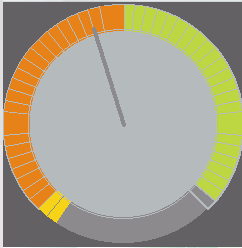
\includegraphics[width=1.25in]{./images/cont1/Viz_1_10}}
		\caption{\textbf{Viz1.} A combination bar graph and fuel gauge-style visualization. }\label{fig:viz1}
	\end{subfigure}
\quad
	\begin{subfigure}[t]{1.25in}
		\centering
		\setlength\fboxsep{0pt}
\setlength\fboxrule{0.5pt}
\fbox{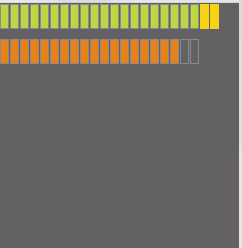
\includegraphics[width=1.25in]{./images/cont1/Viz_2_5}}
		\caption{\textbf{Viz2.} A bar graph style, requires minimal space.}\label{fig:viz2}
	\end{subfigure}
\quad
	\begin{subfigure}[t]{1.25in}
		\centering
		\setlength\fboxsep{0pt}
\setlength\fboxrule{0.5pt}
\fbox{
\includegraphics[width=1.25in]{./images/cont1/Viz_3_3}}
		\caption{\textbf{Viz3.} A simple fuel gauge visualization. The position of the needle and the color of the background indicate balance.}\label{fig:viz3}
	\end{subfigure}
\quad
	\begin{subfigure}[t]{1.25in}
		\centering
		\setlength\fboxsep{0pt}
\setlength\fboxrule{0.5pt}
\fbox{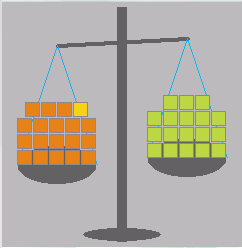
\includegraphics[width=1.25in]{./images/cont1/Viz_4_4}}
		\caption{\textbf{Viz4.} A physical metaphor of a balance scale. Each CHIP is represented by a block. }\label{fig:viz4}
	\end{subfigure}
\quad
	\begin{subfigure}[t]{1.25in}
		\centering
		\setlength\fboxsep{0pt}
\setlength\fboxrule{0.5pt}
\fbox{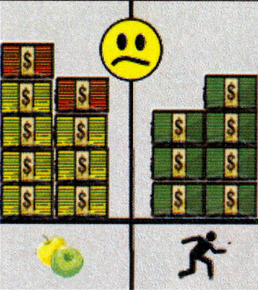
\includegraphics[width=1.25in]{./images/cont1/money}}
		\caption{\textbf{Viz5.} This visualization incorporates money and affective feedback. }\label{fig:money}
	\end{subfigure}
\quad
	\begin{subfigure}[t]{1.25in}
		\centering
		\setlength\fboxsep{0pt}
\setlength\fboxrule{0.5pt}
\fbox{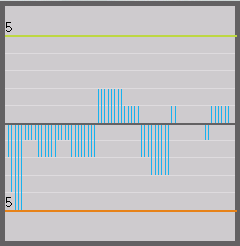
\includegraphics[width=1.25in]{./images/cont1/Viz_6_1}}
		\caption{\textbf{Graph1.} A chart showing change in balance over time. }\label{fig:graph1}
	\end{subfigure}
\quad
	\begin{subfigure}[t]{1.25in}
		\centering
		\setlength\fboxsep{0pt}
\setlength\fboxrule{0.5pt}
\fbox{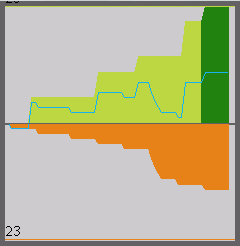
\includegraphics[width=1.25in]{./images/cont1/Viz_8_4}}
		\caption{\textbf{Graph2.} A chart showing change in balance over time, and summed up. }\label{fig:graph2}
	\end{subfigure}


	\caption{Paper prototype visualizations}\label{fig:1}
\end{figure}


\subsection{Results and Discussion}
We rated visualizations based on the number of No. 1 rankings it received.  

In the graph section, we saw that participants strongly preferred Graph2, giving it 10 No. 1 rankings. However, feedback overall was that the graphs were challenging to understand at a glance, and needed more explanation. 

In the visualization section, five participants ranked Viz1 No. 1, making it clearly preferred. Participants liked the ``meter'' and the comparison it provided (P2). It was also remarked to be ``clear, straightforward'', that it ``seems useful'' and ``shows a good balance [of detail]'' (P5).  Viz3 received all No. 4 and No. 5 rankings, because it ``does not show progress and amounts'' (P12), and is ``more confusing'' (P7) . Viz5 received a wider range of rankings, the feedback on it was strong (it is ``a little too judgmental'', and ``not neutral enough'' [P3];P5: ``means nothing with respect to food, smileys are annoying''; P2: ``faces are more discouraging than encouraging-critique''). 
 
Feedback from users indicated that Viz1 is the preferred visualization. Participants liked that it showed the current energy balance and progress toward daily goals or targets, for both energy intake and expenditure. Feedback indicates that the most simple feedback shown (direction and magnitude of energy imbalance, Viz3) does not show enough information and is unsatisfying. Generally, participants found the time-based visualizations too complicated to quickly understand. They also did not believe that the depiction of energy balance over time was useful information. 

Feedback also indicated that participants felt the physical metaphors, such as the scales depicted in Viz4 and Viz5, were too symbolically rich. The imagery was too evocative for simple feedback. The scale metaphor reminded users that if their energy balance was off, their own scale would be tipping. 

Participants did not like the use of money to represent caloric intake and expenditure. While the money ``earned versus spent'' metaphor could be powerful to communicate the ``calories in equals calories out'' concept, people reported that both money and weight were too emotionally charged and they did not want to put the two together. The smiley faces in Viz5, while encouraging when the user is meeting their target, can be discouraging when the user is struggling. Indeed, this is consistent with \cite{consolvo_flowers_2008}, which explores communicating positive and negative affect in feedback mechanisms. 

\section{Prototype, V1 (Feature Phone \& USDA Food Database)}
The next phase of the BALANCE project was the design and development of the first mobile phone prototype. Three things informed the design of this prototype: a review of existing related products (to identify key desired features); a paper prototype process; and the visualization feedback process described above. 

This prototype was built on the Symbian S60 feature phone platform (a top-of-the-line mobile phone platform at the time). Characteristics of mobile phones running the Symbian S60 platform included a relatively powerful processor and ample storage, the ability to develop and run custom software, and high quality cameras. However, they had small displays and 12-key keypads. 

This prototype used the common, freely available USDA Standard Reference. food database (SR19) \citep{u.s._department_of_agriculture_usda_2006}. We added an index based on the FOOD\_DES.FoodName column.  



\begin{figure}	
	\centering
	\begin{subfigure}[t]{1.25in}
		\centering
		\setlength\fboxsep{0pt}
\setlength\fboxrule{0.5pt}
\fbox{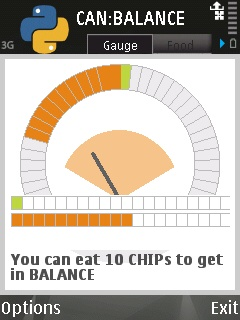
\includegraphics[width=1.25in]{./images/cont1/fig3a}}
		\caption{The home screen depicting overall balance.}\label{fig:fig3a}
	\end{subfigure}
\quad
\begin{subfigure}[t]{1.25in}
		\centering
		\setlength\fboxsep{0pt}
\setlength\fboxrule{0.5pt}
\fbox{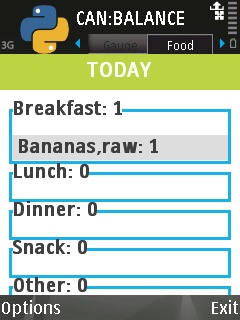
\includegraphics[width=1.25in]{./images/cont1/fig3b}}
		\caption{The food diary, to enter energy intake.}\label{fig:fig3b}
	\end{subfigure}
\quad
\begin{subfigure}[t]{1.25in}
		\centering
		\setlength\fboxsep{0pt}
\setlength\fboxrule{0.5pt}
\fbox{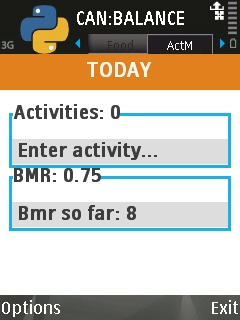
\includegraphics[width=1.25in]{./images/cont1/fig3c}}
		\caption{The activity diary, or energy expenditure.}\label{fig:fig3c}
	\end{subfigure}
\quad
\begin{subfigure}[t]{1.25in}
		\centering
		\setlength\fboxsep{0pt}
\setlength\fboxrule{0.5pt}
\fbox{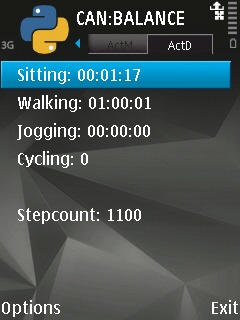
\includegraphics[width=1.25in]{./images/cont1/fig3d}}
		\caption{Sensed activity data from the MSB.}\label{fig:fig3d}
	\end{subfigure}

	\caption{Nokia prototype main screens. }\label{fig:nokiaMainScreens}
\end{figure}


\subsection{Description}
The BALANCE software consisted of four main screens (see Figure \ref{fig:nokiaMainScreens}): The overall balance visualization (Figure \ref{fig:fig3a}), the food diary that shows which foods have been entered today (\ref{fig:fig3b}), and two activity screens. The first activity screen (\ref{fig:fig3c}) shows both intentional activity not detected by the MSB (e.g., water sports such as swimming) and energy expenditure due to base metabolic rate. Base metabolic rate (BMR) is the number of calories a body uses for basic metabolic processes such as breathing. The second activity screen (Figure \ref{fig:fig3d}) shows activity detected by the MSB unit and its contribution to overall energy expenditure. 

\begin{figure}	
	\centering
	\begin{subfigure}[t]{1.25in}
		\centering
		\setlength\fboxsep{0pt}
\setlength\fboxrule{0.5pt}
\fbox{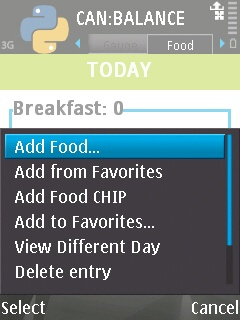
\includegraphics[width=1.25in]{./images/cont1/fig4a}}
		\caption{Select `Add Food' menu item.}\label{fig:fig4a}
	\end{subfigure}
\quad
\begin{subfigure}[t]{1.25in}
		\centering
		\setlength\fboxsep{0pt}
\setlength\fboxrule{0.5pt}
\fbox{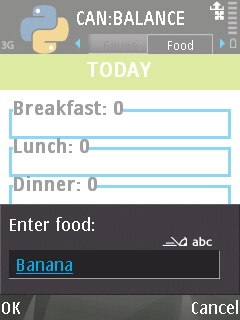
\includegraphics[width=1.25in]{./images/cont1/fig4b}}
		\caption{Enter the name of the food eaten. }\label{fig:fig4b}
	\end{subfigure}
\quad
\begin{subfigure}[t]{1.25in}
		\centering
		\setlength\fboxsep{0pt}
\setlength\fboxrule{0.5pt}
\fbox{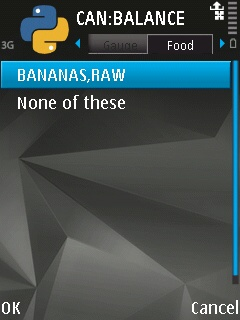
\includegraphics[width=1.25in]{./images/cont1/fig4c}}
		\caption{The software first displays previously used entries with the given name.}\label{fig:fig4c}
	\end{subfigure}
\quad
\begin{subfigure}[t]{1.25in}
		\centering
		\setlength\fboxsep{0pt}
\setlength\fboxrule{0.5pt}
\fbox{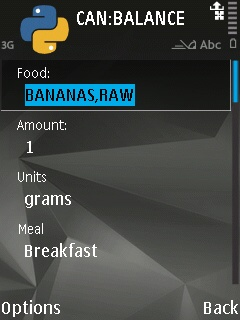
\includegraphics[width=1.25in]{./images/cont1/fig4d}}
		\caption{Selecting the desired food shows this screen, where details about the food entry can be specified. }\label{fig:fig4d}
	\end{subfigure}
\quad
\begin{subfigure}[t]{1.25in}
		\centering
		\setlength\fboxsep{0pt}
\setlength\fboxrule{0.5pt}
\fbox{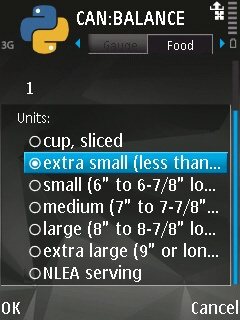
\includegraphics[width=1.25in]{./images/cont1/fig4e}}
		\caption{Selecting the serving amount unit. Some serving units are very specific and natural. }\label{fig:fig4e}
	\end{subfigure}
\quad
\begin{subfigure}[t]{1.25in}
		\centering
		\setlength\fboxsep{0pt}
\setlength\fboxrule{0.5pt}
\fbox{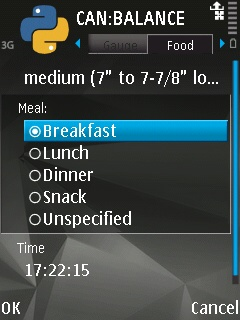
\includegraphics[width=1.25in]{./images/cont1/fig4f}}
		\caption{Selecting the meal for this food.}\label{fig:fig4f}
	\end{subfigure}
	\caption{Nokia prototype: Add known food}\label{fig:fig4}
\end{figure}

In Figure \ref{fig:fig4}, the screenshots depict the process of adding \textit{Banana} to today's food diary. The user first selects ``Add Food'' from the menu. He then types in the term using T9 or multitap. On submit, a list of foods that the user has entered before is shown. The user selects \textit{Banana, Raw}, and is shown a screen to modify the amount, time, and meal eaten. The USDA database provides default serving sizes in grams. Some entries have alternate serving sizes available. For \textit{Banana, Raw}, the serving sizes include ``cup, sliced'' and ``small (6'' to 6 7/8'' long). Finally, the food entry is created. When the food entry is created, the food name appears on the food diary screen and the main visualization is updated. 

\begin{figure}	
	\centering
	\begin{subfigure}[t]{1.25in}
		\centering
		\setlength\fboxsep{0pt}
\setlength\fboxrule{0.5pt}
\fbox{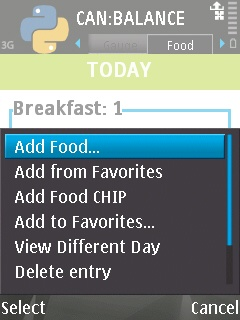
\includegraphics[width=1.25in]{./images/cont1/fig5a}}
		\caption{To make a new food entry, select the `Add Food' menu item. }\label{fig:fig5a}
	\end{subfigure}
\quad
\begin{subfigure}[t]{1.25in}
		\centering
		\setlength\fboxsep{0pt}
\setlength\fboxrule{0.5pt}
\fbox{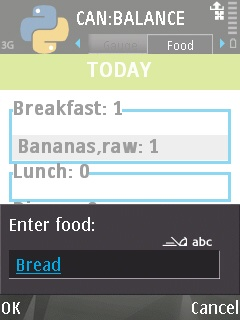
\includegraphics[width=1.25in]{./images/cont1/fig5b}}
		\caption{Enter the food name. }\label{fig:fig5b}
	\end{subfigure}
\quad
\begin{subfigure}[t]{1.25in}
		\centering
		\setlength\fboxsep{0pt}
\setlength\fboxrule{0.5pt}
\fbox{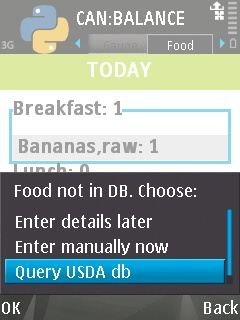
\includegraphics[width=1.25in]{./images/cont1/fig5c}}
		\caption{When the food name has not been used before, the user is given the option to either bookmark the entry to fill out later, create a manual entry using the nutrition facts label now, or query the database.}\label{fig:fig5c}
	\end{subfigure}
\quad
\begin{subfigure}[t]{1.25in}
		\centering
		\setlength\fboxsep{0pt}
\setlength\fboxrule{0.5pt}
\fbox{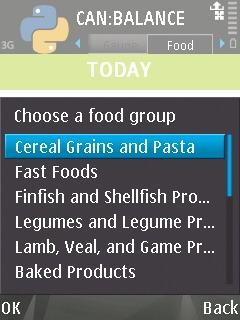
\includegraphics[width=1.25in]{./images/cont1/fig5d}}
		\caption{When there are many entries, the user is asked to choose a food group to filter the results. }\label{fig:fig5d}
	\end{subfigure}
\quad
\begin{subfigure}[t]{1.25in}
		\centering
		\setlength\fboxsep{0pt}
\setlength\fboxrule{0.5pt}
\fbox{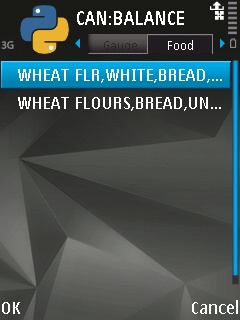
\includegraphics[width=1.25in]{./images/cont1/fig5e}}
		\caption{All matching entries are displayed alphabetically. }\label{fig:fig5e}
	\end{subfigure}
\quad
\begin{subfigure}[t]{1.25in}
		\centering
		\setlength\fboxsep{0pt}
\setlength\fboxrule{0.5pt}
\fbox{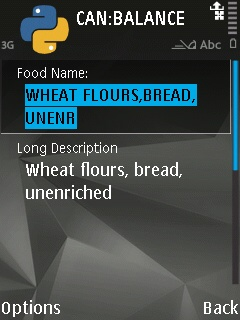
\includegraphics[width=1.25in]{./images/cont1/fig5f}}
		\caption{The user is given a chance to edit the food name to something more recognizable if desired. }\label{fig:fig5f}
	\end{subfigure}
	\caption{Nokia prototype: Adding newly encountered (previously unused) food}\label{fig:fig5}
\end{figure}

One primary goal of this project was for users to be able to quickly and accurately enter exactly how many calories they had consumed. This required finding the most appropriate, exact food and entering it in the exact amount, right after eating. The process of finding food needed to be fast to minimize interruption to the user. Queries to the entire food database took a long time to execute (this is described in further detail later), so to improve performance we separated the database into two separate databases: the entire USDA database and foods the user has entered before. The second database is called the \textit{personal database}. We justify the use of the personal database because many people have a relatively small number of foods they eat on a regular basis (\citep{jastran_eating_2009}). The smaller personal database can be populated over time.  The personal database reduces the amount of time it takes to find a food because it contains fewer foods than the USDA database. This results in a lower query response time. It is also more likely to return the desired food, because it is populated with foods the user has eaten before. 

When the user submits a search, the app first checks the personal database. This first check is fast because the personal database is small. If there are no results, the user is asked whether they want to ``enter later'', ``enter manually'', or ``look up in USDA db''. The ``enter later'' option is essentially a bookmark. This provides a quick alternative to finding the food in the USDA database, which is time-consuming. The ``enter manually'' option provides a form for the user to make an entry based on the Nutrition Information panel required to be printed on all packaged foods. 

Figure \ref{fig:fig5} shows the process of entering a food (\textit{bread}) that has not been entered in the food diary before; therefore, it does not exist in the personal database. When the user query \textit{bread} is not found in the database, the user is given the option to look it up in the USDA database (Figure \ref{fig:fig4c}). If this option is selected and the query returns with foods that belong in more than one food class, the food classes are listed first. Choosing a food class filters the food results list. In this example, the search for \textit{bread} resulted in foods in 14 food classes, which is displayed in three pages of choices (Figure \ref{fig:fig4d}). Choosing \textit{Cereal Grains and Pasta} displays the relevant food results (Figure \ref{fig:fig4e}). The users chooses the item they ate and can modify the name or details. The new food is added to the personal database so that the next time the user enters that food, it can be found faster. Finally, the user specifies the details needed to add the item to the food diary. 

\subsection{Database Optimization and Querying}
One challenge of working with databases is identifying queries the user will make, or want to make, and the expected results. Then, we generate a database query to provide the results. Generating a query based on user input has performance implications, particularly when working with text. Queries on a string column are slower than other data types. Searching for strings with wildcards further degrades the response time. 

In the BALANCE software, a user provides a basic query and the software generates a query based on that user input. Each word the user provides becomes a predicate in the query. This approach results in queries that are known to have poor performance, but this is necessary to account for the ordering of relevant terms in the database. Table \ref{tab:table1} gives some examples of food terms that a user might enter and some example results. As we see in the example of \textit{cream cheese}, if the query had been restricted to ``LIKE �*cream cheese*�'', ``cheese, cream'' would not be returned as a result. There is no simple, systematic way to consistently reorder queries the user provides to match the inconsistent entries in the database. 
 
% Table generated by Excel2LaTeX from sheet 'Sheet1'
\begin{table}[htbp]
\small
  \centering
  \caption[Examples of a user query and results.]{Examples of a user's initial query, how it gets converted into a database query, and some example results. Note that some queries can generate many different, potentially unexpected results. The generated query and subsequent results do not preserve the user's original word ordering. }
    \begin{tabular}{p{1.5in}p{2.2in}p{1.75in}}

    \toprule
%\vtop{\vskip -\ht\strutbox }
    \textbf{User Search Request} & \textbf{Query WHERE clause} & \textbf{Example results} \\
    \midrule
    \textit{cheese} & LIKE �*cheese*�  & Cheese, Cheddar \newline
Cheese, Cream \newline
Bagel with Cream Cheese \newline
Pizza, Cheese and Pepperoni \\
& & \\
   \textit{cream cheese} & LIKE �*cream*� AND LIKE �*cheese*� & Cheese, Cream \newline 
Bagel with Cream Cheese \\
    \bottomrule
    \end{tabular}%
  \label{tab:table1}%
\end{table}%


\subsection{Observations}
Evaluating the first prototype of the BALANCE software revealed many unanticipated difficulties. In this section, I describe the observed problems. They generally relate to the process of finding and choosing a food for the food diary. A summary list is shown below, and I further describe each difficulty: 
\begin{enumerate*}
\item Text entry was difficult. 
\item Querying the database was slow. 
\item Finding and choosing a specific food. 
\begin{itemize*}
\item Using food class to filter search results. 
\item Long names that did not fit on the screen. 
\item No entry for commonly prepared foods. 
\item For some foods, many variations to choose from. 
\end{itemize*}

\end{enumerate*}

\subsubsection{Text entry was too hard}
The 12-key keypad required users to use multi-tap or T9 to enter the names of food they have eaten. This is very difficult to do for foods with long names. When users wanted to enter a food, they needed to decide whether to type in a long, detailed food name, or a short, broad food name. The long and detailed name will likely return fewer food results, but there is a greater chance that the target food is missed. Using a short food name for a query could result in many responses to navigate. 

\textbf {Recommendation: } To appeal to less tech-savvy consumers, provide a more comfortable means of text input. 

\subsubsection{Too long to search}
As discussed above, user input is converted into a query that is known to have poor performance. This is partly due to a mismatch between what the user wants to search for (\textit{cream cheese}) and how it may be stored in the database (``cheese, cream'' or ``bagel, with cream cheese''). It is important that the software returns all of the results. 

The long search time is primarily due to the limited resources on the mobile phone. The database available on the mobile platform has reduced capabilities as compared to those available on a desktop or in a high performance computing environment. The limited processing power of the device magnifies the limitations of the database. 

\textbf {Recommendation:} Faster hardware, improve the filtering process.
 
\subsubsection{It was difficult to find and choose a food}
After entering a food query and waiting for the search to return, a user needs to choose the desired food from all of the results. 
Using food class to filter search results. As noted earlier, if the results are from just one food class, the entire list of results is immediately shown. If there are results in multiple food classes, the list of food classes is shown to allow the user to choose the most appropriate. To find the target food, the user must choose from a potentially long list of food classes (the results for the query \textit{bread} include 16 food classes). Some of the food classes are difficult to distinguish. For example, the food classes for \textit{Bread} includes both ``Cereal Grains and Pasta'' and ``Baked Goods''. This requires the user to make a decision, and users unfamiliar with the food classes are not sure which to choose. 

\textbf{Recommendation: }Do not force the user to think about arbitrary food classes. Provide guidance about what each food class represents. Provide a preview or a few items of that food class to demonstrate what kinds of foods it contains. 

\subsubsection{Long names do not fit on the screen.}
The USDA database contains food descriptions that are long and descriptive. For example, a typical entry for the query ``Steak'' is ``Beef, short loin, porterhouse steak, separable lean and fat, trimmed to 1/4'' fat, USDA choice, raw''.  The alternative ``short'' description is a similar entry using defined abbreviations: ``Beef, shrt loin,prtrhs steak,ln,1/4'' fat,usda choic,raw''. Neither of these descriptions display well on the small screen size of the target device. If they are displayed one entry per line in a font that is comfortable to read, not enough words are shown to distinguish one entry from another. If the description is shown on multiple lines, only one or two entries can be shown at a time. Forcing the user to select one to see more detail and then returning to the list screen is time consuming and frustrating. 
 
\begin{figure}[ t ]
\begin{center}

\setlength\fboxsep{0pt}
\setlength\fboxrule{0.5pt}
\fbox{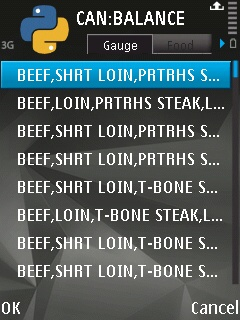
\includegraphics [ width=1.25in ]{./images/cont1/fig6}}

\caption{Nokia prototype: `Steak' results}
\label{fig:fig6}
\end{center}
\end{figure}

\textbf {Recommendation: }Use a larger display with higher resolution. Use a database that has more useful short descriptions. Structure the database to provide a short food name, a short description, and a detailed description. 

\subsubsection{No entries for common prepared foods. }
The USDA database is that it did not include many prepared foods, such as those purchased at a grocery store or restaurant. The database contains food entries from only 60 manufacturers. This includes some of the major food manufacturers in the US (e.g. Burger King, Kellogg, Nestle, McDonalds). However, users expect that if they can purchase a food (e.g., it has a UPC code), then it will be in the database. 

\textbf{ Recommendation:} Choose a database that includes a more comprehensive list of prepared foods. 

\subsubsection{For some foods, many items to choose from.}  For some foods, there are many entries that appear very similar. For example, a query for \textit{cheese} in the ``Dairy and Egg Products'' Food Class has 44 entries. The cheese entries include: cheese, blue; cheese, brick; cheese, brie;  cheese, camembert; cheese, cheddar; etc. Some results may be unfamiliar to a user, but the text of each result is noticeably different from the others. The results for \textit{Porterhouse} (steak) are not so clearly different. The list below displays the full name of six results for \textit{porterhouse}: 

\begin{itemize*}
\item Beef, short loin, porterhouse steak, separable lean and fat, trimmed to 0'' fat, all grades, cooked, broiled
\item Beef, short loin, porterhouse steak, separable lean and fat, trimmed to 0'' fat, USDA choice, cooked, broiled
\item Beef, short loin, porterhouse steak, separable lean and fat, trimmed to 0'' fat, USDA select, cooked, broiled
\item Beef, short loin, porterhouse steak, separable lean only, trimmed to 0'' fat,  all grades, cooked, broiled
\item Beef, short loin, porterhouse steak, separable lean only, trimmed to 0'' fat, USDA choice, cooked, broiled
\item Beef, short loin, porterhouse steak, separable lean only, trimmed to 0'' fat, USDA select, cooked, broiled
\end{itemize*}

The six results vary on two factors: whether the item contains only the separable lean meat, or the meat and fat; and the grade rating of the meat, USDA choice, select, or any. 

This amount of detail confuses users. They report uncertainty about which one most accurately reflects the food they ate, and question whether the difference between all these results is significant. Additionally, the amount of distinguishing detail for this entry makes users wonder if they should be capturing that amount of detail for all of the foods they enter. This compounds the previous problem of not being able to find prepared foods: given the level of detail required to document a piece of steak, how should the user document a piece of pizza, which vary wildly due to toppings and preparation?

\textbf{Recommendation:} Use a database that was designed for use by a consumer rather than an expert. 

The overall process to add food to the food diary is too long, due to all of the factors described in detail above. For the BALANCE project, it was important that users are able to enter foods quickly, so that they are able to enter food throughout the day and ensure the fuel-gauge visualization is properly updated. 

\subsection{Discussion}
The Nokia-USDA BALANCE prototype exposed some inherent challenges of designing and developing a food diary for a mobile phone. The challenges are due partly to the database, and partly from using a device with limited interaction modes to navigate a challenging data environment. Our target population is a general population, not necessarily very comfortable entering text via multitap or T9. This challenge of text entry magnifies the problem of querying the database and navigating the results. 

One conclusion from this process was to use a different mobile phone. The original Symbian S60 device was much friendlier to use and more powerful than previous smartphones, but the target population had little smartphone experience.  Text entry was one of the biggest barriers: the 12-key keypad with multitap or T9 input was not comfortable to most consumers. 

The database negatively impacted the navigation and performance. Database entries were not well suited to the mobile phone display, and the query process on the device was too slow. It is also necessary to have more popularly available packaged or prepared foods, although some of the closely related foods could be collapsed. The importance of the database in self-monitoring or dietary assessment is outlined in \cite{stumbo_considerations_2008}. Indeed, they state ``Mastery of computerized dietary assessment requires an understanding of the database in terms of the naming conventions, the search strategy for finding foods, and data completeness for generic and brand-name foods.'' This is consistent with our experiences. 

\section{Food Databases}
Food diaries have conflicting requirements for the food database. In particular for BALANCE, the database needs to be quick to search (small), yet have the foods that people eat and are looking for (large). It also needs to be able to distinguish between similar items, and use terminology that is familiar to the target user population. Grouping into friendly and familiar food groups or classes will help users to find food in the database by providing data to filter on or browse. Providing useful, appropriate serving sizes is another helpful feature. For example, the food entries for \textit{Coca Cola} should have commonly available serving sizes to choose from, such as a 12-oz can, a 20-oz bottle, or a 16-oz cup, even though the USDA-defined `typical' serving size for soda is 8 oz. 

The characteristics of food databases can be better appreciated within the historical context. Generally, food databases are used by professionals who are experts in food service, preparation, and evaluation. Hospitals, nursing homes, and other medical facilities use food databases to ensure patients are fed properly, fulfilling individual requirements. They generate menus for days, weeks and months, using the database to ensure proper nutrition for all recipients over time. Nutritionists and registered dietitians use commercial food databases to work with clients who have certain dietary constraints--- either to look up foods that an individual ate and evaluate their diet overall, or to generate a meal plan for an individual and provide detailed information about it. Organizations such as daycares, schools and prisons (particularly if they are government funded) use food databases to ensure that they meet governmental guidelines. Food manufacturers use food databases to generate Nutrition Facts labels for their products. 

For the tasks outlined above, the end user of the database is an expert who is familiar with food systems, organization, and terminology. The user has formal training and uses the database on a regular basis. However, increasingly, food databases have been made available to the general population, usually in the form of a consumer tool to support weight loss. 

Table \ref{tab:foodDbCompare} provides some information on two databases: the USDA (SR21) database we used for the first prototype, and the NPKB that we used for the next version of the software. In addition to containing information for many more foods, it also provides more food serving sizes that could make it easier for users to specify how much they have eaten. It also contains foods from many more manufacturers, which can help address the expectation to find processed or prepared foods in a database. Finally, the NPKB database contains more foods groups, organized in a hierarchical fashion. The large number of food groups and hierarchy may help users find a food they are looking for. 

% Table generated by Excel2LaTeX from sheet 'Sheet2'
\begin{table}[htbp]
\small
  \centering
\begin{minipage}{\textwidth}
\centering

    \begin{tabular}{p{2in}p{1.75in}p{1.75in}}
    \toprule
    \textbf{} & \textbf{USDA} & \textbf{Nutritionist Pro Knowledge Base} \\
    \midrule
    \textbf{Version} & SR21 (Sept 2008) & V44 (Fall, 2009) \\
    \textbf{File size\footnote{Access database file size}} & 16.5 Mb & 135 Mb \\
    \textbf{Number of foods} & 7,412 & 39,194 \\
    \textbf{Number of food servings\footnote{``serving types''}} & 13,087\footnote{Number of records in the `Weight' table.}  & 46,722\footnote{Number of records in the `tblFoodServingTypes' table} \\
    \textbf{Number of serving types} & 1,700  & 5,087 \\
    \textbf{Number of manufacturers} & 60    & 592 \\
    \textbf{Number of recipes} &       & 783 \\
    \textbf{Food groups} & 24    & 369\footnote{Food Classes. Includes entire  hierarchy.}\\
    \textbf{Number of nutrients } & 140   & 90 \\
	\bottomrule~
    \end{tabular}%
\end{minipage}
  \caption{Comparing nutrition databases\label{tab:foodDbCompare}}  
	%
\end{table}%




 
\section{Food Diary: Iterative Design And Evaluation}
In this section, I describe the design and features of the food diary portion of the overall BALANCE project. The challenges identified in the previous section informed the decision to move to a Windows Mobile platform and adopt a commercially available nutrition database to drive the food diary. The combination of the paper prototype user study and Symbian implementation informed the new design on the Windows Mobile platform. The final design was informed by an iterative, user-centered evaluation process. 

Focus groups of 4-5 participants provided user feedback in the design and development process. We convened five focus groups over a seven month period. We provided participants a mobile phone running the food diary software. We asked to track what they eat for three days prior to the focus group. After the three days of tracking and before the focus group, participants completes two usability questionnaires (CSUQ and MPUQ, \citep{lewis_ibm_1995, ryu_reliability_2006}). The focus group was moderated by a team member. Topics focused on what the participants liked, what worked and did not work, and features they would like to see added. Details are in \citet{hughes_balance_2010}. Feedback from the participants in the focus groups provided input to the design and development of the next software iteration. 
We used two metrics to evaluate the overall progress of the iterative process. First, we analyzed usability questionnaire responses over time. These did not show a significant improvement of the usability of the food diary software overall. The other measure of progress we considered was the time between when a participant ate a food and when they entered it in the food diary. We hypothesized that this time would decrease as the food diary improved. This also did not show a significant improvement of the food diary. Details of the analysis are provided in \citet{hughes_balance_2010}. I also discuss the use of these metrics later in this section and in Chapter \ref{cha:cont4}. 

\subsection{Overall Design}
The final version of the BALANCE software ran on a Windows Mobile 6.1 Professional device. We chose this device because it had a large display, a touch screen, and a slide-out QWERTY keyboard. Text input can be done either via the physical QWERTY keyboard or with the ``soft input panel'', on-screen keyboard. We used the NutritionistPro Knowledge Base (NPKB) for the food diary. 

\subsubsection{Food Diary Software}
The primary task for the food diary is to enable users to find a food that has been eaten from a database, specify how much of it they ate, and save a record of it. 

\begin{figure}	
	\centering
	\begin{subfigure}[t]{1.25in}
		\centering
		\setlength\fboxsep{0pt}
\setlength\fboxrule{0.5pt}
\fbox{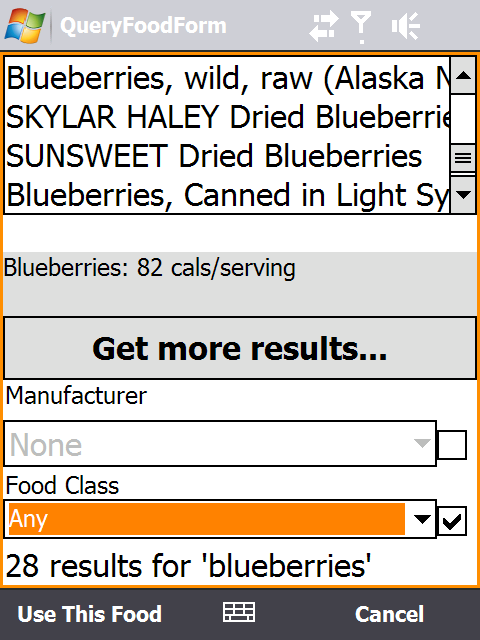
\includegraphics[width=1.25in]{./images/cont1/fig7a}}
		\caption{The BALANCE food diary main screen.}\label{fig:fig7a}
	\end{subfigure}
\quad
\begin{subfigure}[t]{1.75in}
		\centering
		\setlength\fboxsep{0pt}
\setlength\fboxrule{0.5pt}
\fbox{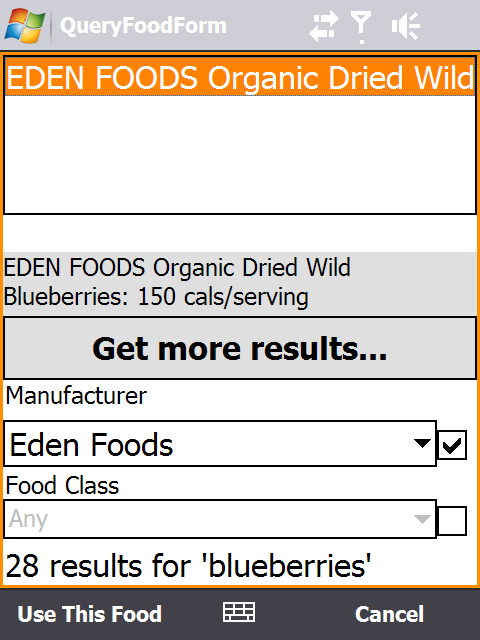
\includegraphics[width=1.75in]{./images/cont1/fig7b}}
		\caption{Entering the query term. Common or previously used results appear.}\label{fig:fig7b}
	\end{subfigure}
\quad
\begin{subfigure}[t]{1.75in}
		\centering
		\setlength\fboxsep{0pt}
\setlength\fboxrule{0.5pt}
\fbox{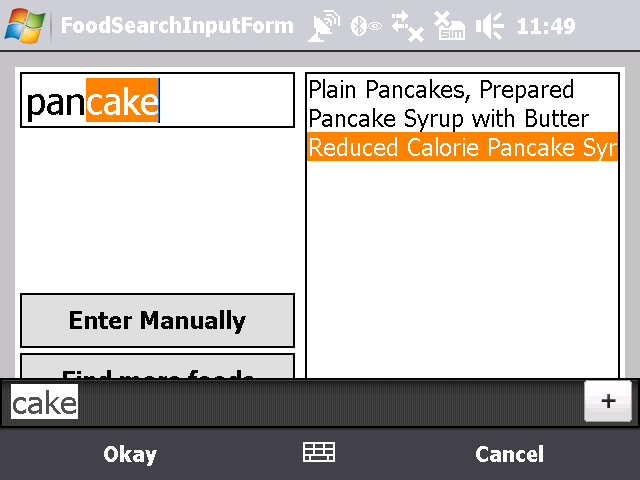
\includegraphics[width=1.75in]{./images/cont1/fig7c}}
		\caption{The user continues typing to filter out this list. }\label{fig:fig7c}
	\end{subfigure}
\quad
\begin{subfigure}[t]{1.25in}
		\centering
		\setlength\fboxsep{0pt}
\setlength\fboxrule{0.5pt}
\fbox{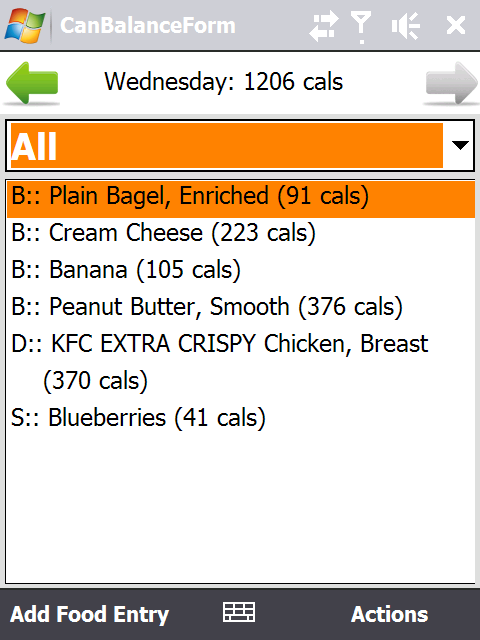
\includegraphics[width=1.25in]{./images/cont1/fig7d}}
		\caption{An exact match was not found, so more results were loaded. This list can be filtered by manufacturer or food class.}\label{fig:fig7d}
	\end{subfigure}
\quad
\begin{subfigure}[t]{1.25in}
		\centering
		\setlength\fboxsep{0pt}
\setlength\fboxrule{0.5pt}
\fbox{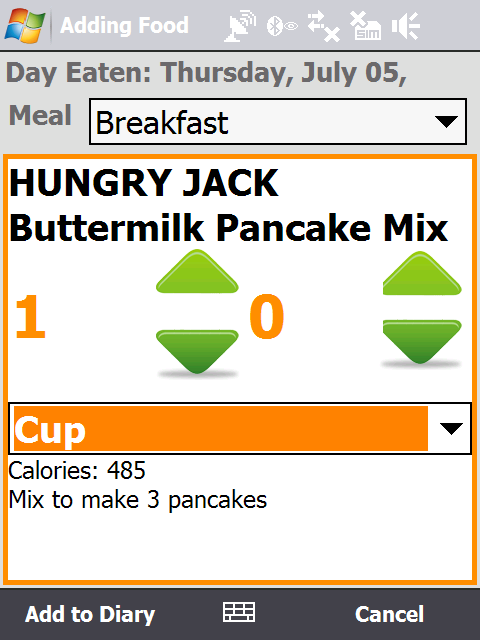
\includegraphics[width=1.25in]{./images/cont1/fig7e}}
		\caption{Creating the entry by specifying the day it was eaten, the meal, and the amount. }\label{fig:fig7e}
	\end{subfigure}
\quad
\begin{subfigure}[t]{1.25in}
		\centering
		\setlength\fboxsep{0pt}
\setlength\fboxrule{0.5pt}
\fbox{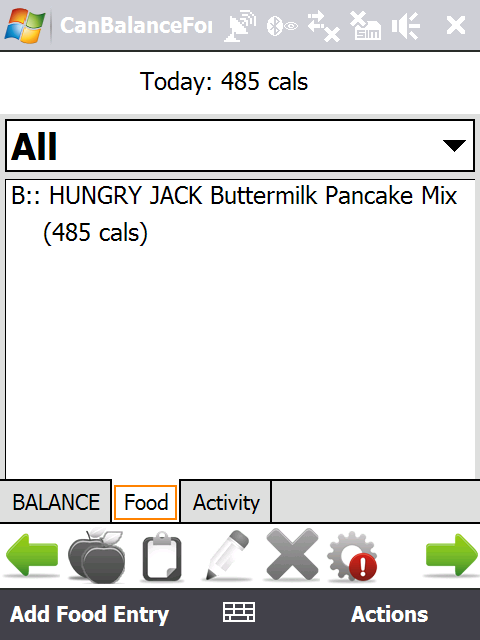
\includegraphics[width=1.25in]{./images/cont1/fig7f}}
		\caption{The new food entry is now displayed on the food diary main screen. }\label{fig:fig7f}
	\end{subfigure}
	\caption{WinMobile food diary.}\label{fig:fig7}
\end{figure}


Figure \ref{fig:fig7} shows the process of adding a food to the diary. The application starts with a list of food that has been eaten today (\ref{fig:fig7a}). The ``Add Food Entry'' button displays a screen that allows the user to start typing an entry (\ref{fig:fig7b}). As the user types, a list of common or recently eaten foods populates the display (\ref{fig:fig7c}). If the user sees what they want, they can either select it, choose to ``Enter Manually'' (create a new entry based on the Nutrition Information label on the package), or ``Find more'', which searches the entire food database (\ref{fig:fig7d}). This list can be filtered by manufacturer and food class  (\ref{fig:fig7d}). Once a food is selected, the user specifies what time they ate the food, which meal it should be counted with, and how much of it they ate  (\ref{fig:fig7e}). The entry is then saved and shown on the daily food list  (\ref{fig:fig7f}). 

\subsection{Selected Features and Feedback}
Throughout the iterative design process, we aimed to improve the existing functionality and add features as necessary. In this section, I detail some of the features that evolved based on user feedback. 

\subsubsection{Touch-friendly screen design }

We chose the final device for its touch-sensitive screen. We believed the touch interface could help reduce the time required to create a food entry, whether the touch was provided by a fingernail or a stylus. Initially, the food diary design supported touch interaction by using traditional WinMobile interface widgets scaled to respond to fingernail touches. This required the widgets to be larger than widgets sized to support stylus interaction (see \ref{fig:fig8}). However, early in the feedback process, users reported that they did not like the stylus. This indicated that they were using it, even though the design did not intend to require it. Although the traditional widgets were scaled to respond to fingernail touches, the appearance invited the use of a stylus for interaction. Additionally, users provided valid complaints against the use of a stylus: it was too small to hold comfortably; users were afraid of losing it; and it was time consuming to take it out and put it back. 

In response to user feedback about the use of the stylus, we redesigned the interface to use custom widgets that invited fingernail touches (see \ref{fig:fig8b} and \ref{fig:fig8c}). Users remarked on the ``friendliness'' and ``cheeriness'' of the new widgets. 

\begin{figure}[tbh]
	\centering
	\begin{subfigure}[t]{1.25in}
		\centering
		\setlength\fboxsep{0pt}
\setlength\fboxrule{0.5pt}
\fbox{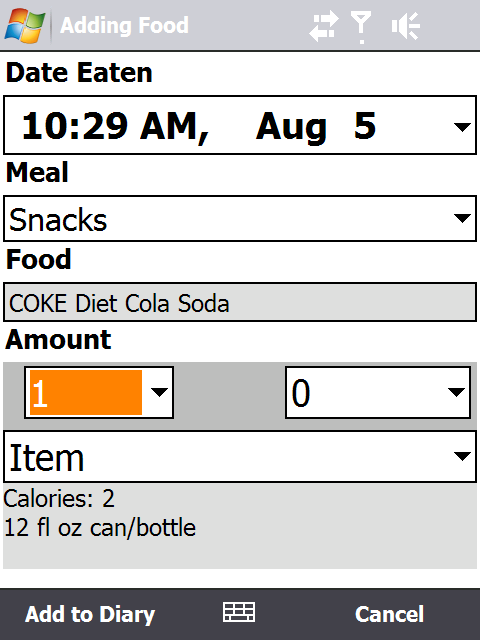
\includegraphics[width=1.25in]{./images/cont1/fig8a}}
		\caption{The first design. The design and layout is typical of a Windows Mobile or PDA software that depends on the use of a stylus. }\label{fig:fig8a}
	\end{subfigure}
\quad
\begin{subfigure}[t]{1.25in}
		\centering
		\setlength\fboxsep{0pt}
\setlength\fboxrule{0.5pt}
\fbox{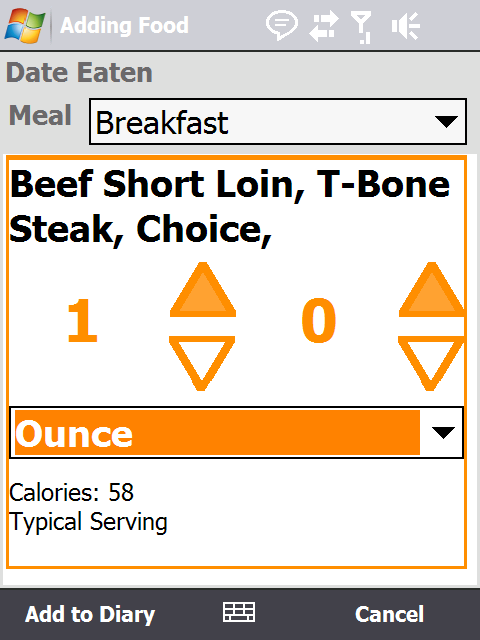
\includegraphics[width=1.25in]{./images/cont1/fig8b}}
		\caption{A revision, with large, finger touch friendly buttons to modify the serving amount.  }\label{fig:fig8b}
	\end{subfigure}
\quad
\begin{subfigure}[t]{1.25in}
		\centering
		\setlength\fboxsep{0pt}
\setlength\fboxrule{0.5pt}
\fbox{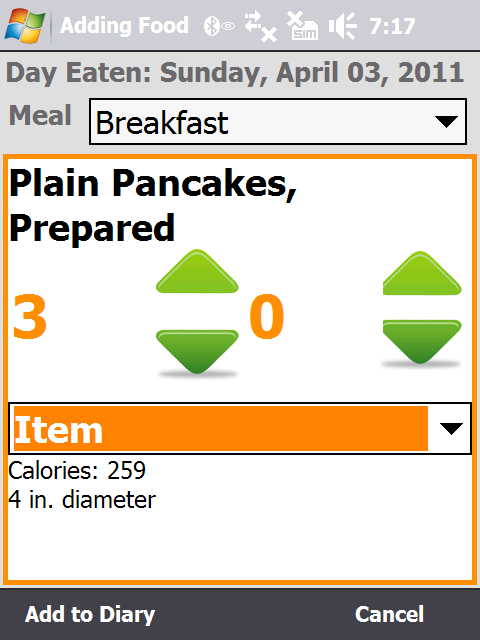
\includegraphics[width=1.25in]{./images/cont1/fig8c}}
		\caption{The final version.}\label{fig:fig8c}
	\end{subfigure}
	\caption{Evolution of serving size specification to make it more touch-friendly.}\label{fig:fig8}
\end{figure}

\subsubsection{Create new food database entry}
The NPKB contained many foods, but users still reported encountering foods that were not in the database. This resulted in the ability to add a new food to the database, using information from the Nutrition Facts label that all packaged foods are required to have. After the entry is created, it shows up in the quick-search results with other common and recently used foods. 
 
\begin{figure}[ t ]
\begin{center}

\setlength\fboxsep{0pt}
\setlength\fboxrule{0.5pt}
\fbox{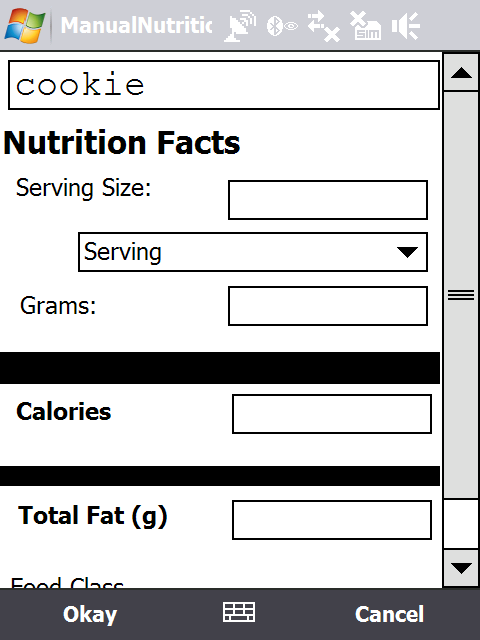
\includegraphics[ width =1.25in ]{./images/cont1/fig9}}
\caption{Add a new manual entry to food diary when the database does not have the desired food. }
\label{fig:fig9}
\end{center}
\end{figure}

\subsubsection{Favorite foods and meals}
Focus group participants repeatedly asked for shortcuts and customization features. In addition to the ability to add a new food to the database described above, participants wanted the ability to bookmark favorite foods and meals. The favorite meals feature is shown in Figure \ref{fig:fig10}. Figure \ref{fig:fig10a} shows the list of all meals that have been marked as a favorite. When the user wants to enter the favorite meal, s/he selects it from the list. Figure \ref{fig:fig10b} shows all of the items in the meal, as well as the amount. The time defaults to the current time (rounded to the nearest 15 minutes). The saved favorite meal includes the meal specification (breakfast, dinner, etc.), which populates the meal widget. The details of the meal can be modified to reflect the current meal (\ref{fig:fig10c}). Finally, when the user confirms, all of the items in the meal are added to the food diary (\ref{fig:fig10d}). 

\begin{figure}	
	\centering
	\begin{subfigure}[t]{1.25in}
		\centering
		\setlength\fboxsep{0pt}
\setlength\fboxrule{0.5pt}
\fbox{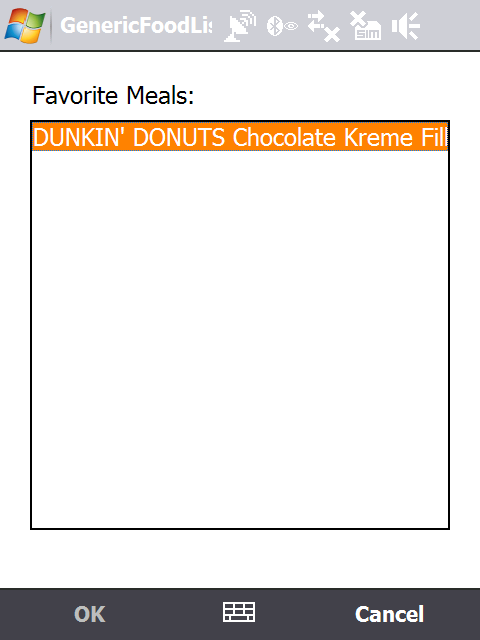
\includegraphics[width=1.25in]{./images/cont1/fig10a}}
		\caption{The list of meals saved as `Favorite'.}\label{fig:fig10a}
	\end{subfigure}
\quad
\begin{subfigure}[t]{1.25in}
		\centering
		\setlength\fboxsep{0pt}
\setlength\fboxrule{0.5pt}
\fbox{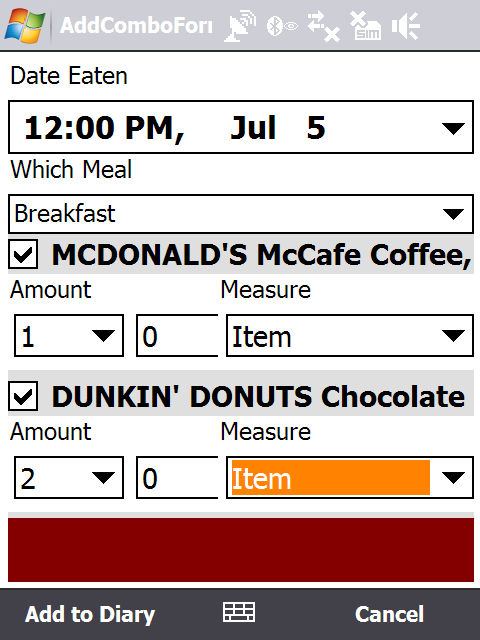
\includegraphics[width=1.25in]{./images/cont1/fig10b}}
		\caption{Selecting a meal shows a screen that lists each item in the meal, including serving sizes. In this case, one McDonald's coffee and two donuts. }\label{fig:fig10b}
	\end{subfigure}
\quad
\begin{subfigure}[t]{1.25in}
		\centering
		\setlength\fboxsep{0pt}
\setlength\fboxrule{0.5pt}
\fbox{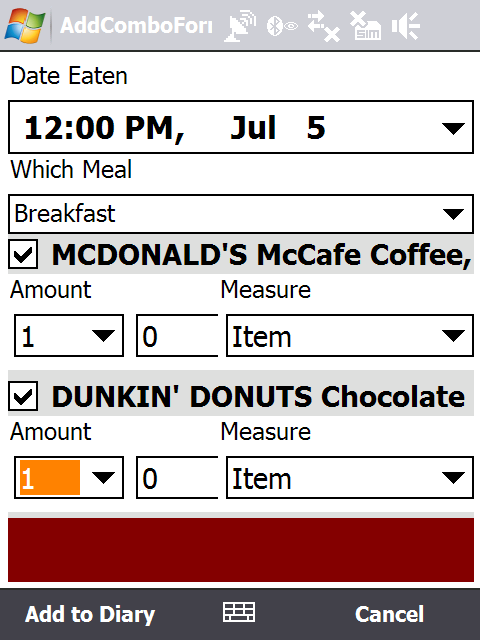
\includegraphics[width=1.25in]{./images/cont1/fig10c}}
		\caption{The amounts can be modified to reflect the current meal. }\label{fig:fig10c}
	\end{subfigure}
\quad
\begin{subfigure}[t]{1.25in}
		\centering
		\setlength\fboxsep{0pt}
\setlength\fboxrule{0.5pt}
\fbox{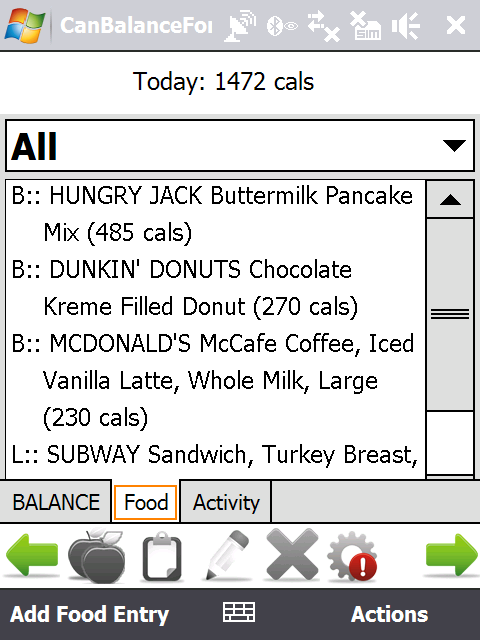
\includegraphics[width=1.25in]{./images/cont1/fig10d}}
		\caption{When entered, each item is added to the daily food list. }\label{fig:fig10d}
	\end{subfigure}

	\caption{Using the favorite meals feature to add entries to the food diary. }\label{fig:fig10}
\end{figure}

\subsection{Database Query Details}
Adopting the commercially available NPKB resulted in a much larger number of foods available to the user. While the USDA database had the user challenge of making it difficult to distinguish between many similar unprocessed foods and relatively few processed/manufactured foods, the NPKB had many more processed and manufactured foods to choose from, which users sometimes found overwhelming. 

In this section, I describe some of the ways we tried to make the query process more user friendly. Rather than describe all the possible improvements we considered, I focus on the final implementation. 

One weakness of the database supported on the Windows Mobile platform (SQL Server CE) is that it does not support full text search. When full text search is available on a database, queries can be made that reflect linguistic characteristics of a given language (such as English). With a FTS capability, one can easily query  not just for a word or a phrase, but a word or a phrase that starts with given text (prefix), inflectional forms of a word (e.g., foot or feet), a word or phrase close to another word or phrase, or a synonymous term. This is valuable in the case of food diaries, because from the user's perspective it is sometimes unclear whether the food diary will have ``Potatoes, Mashed'' or ``Mashed Potatoes'' as an entry. Additionally, consumers in general are familiar with search strategies that employed FTS, whether or not they know enough about it to specify it exactly. Users are able to articulate is that a particular search function ``just knows what I'm looking for'' and ``does the right thing'', linguistically-a search for ``potatoes'' also yields results with ``potato''. 

Full text search also improves the query speeed. The alternative to full text search is a LIKE query based on character patterns. A LIKE query against millions of rows of text data can take minutes to return, while a full text search query can take only seconds (or less) on the same data, depending on the number of rows that are returned. This is due to the pre-built index that full text search generates. 

We attempted to overcome the lack of free-text search on the database by being smart about the queries we generated. However, the more complex a query became, the longer the time to respond, even if the results were ``better''.  In general, our approach favored returning better results faster, rather than minimizing the size of the database. Storage was cheap: we could easily add a larger memory card to the device, but we could not improve the processor. 

To improve the query time and search process, we implemented a lightweight predictive search mechanism. As mentioned above, the system contained two food databases: the large, complete NPKB and a smaller, personalized personal database. The personal database was initially seeded with foods marked as ``common'' or ``generic'' in the NPKB. To improve the responsiveness, there was a table in the personal database that contained the first 3 letters of all words in the food name, description and manufacturer name associated with a food entry. When the user starts typing to search for a food name, after 3 characters are entered, a results box is generated based on an exact string match from that table. As the user continues typing, the list of results is filtered based on that text. If a desired food is not found, the user can ``Find More'', which ends up performing the longer LIKE query on the NPKB. When a food is selected from the NPKB and entered into the food diary, it is also stored in the personal database. The prefix table is then updated. This adds time to the process, but this time is negligible to the time required for the NPKB query. 

\subsection{Metrics}

In this section, I want to talk about the metrics we used to guide the development and evaluation of the software. Specifically, I want to review what we used, how they worked, why they failed, and propose alternate metrics to collect during the final evaluation. 

We defined one measure of software success as the time between when a food was eaten and when it was entered into the diary. This measure did not show  significant improvement, but it did indicate how the software is used. This was supported by feedback in the focus groups. Participants reported that they did not make food entries throughout the day, and were not likely to. Multiple reasons were given for this: sometimes it was just that the person was too busy and could not take the time, and sometimes it was just easier to do it all at once later in the day. Some participants noted that they took advantage of free time, such as waiting for the bus, to review and make food entries. This does not help us to identify if the reluctance to make food entries at the time of eating is due to an inherent tedium in the task, or if the software makes the process more or less challenging. 

This study highlighted the importance of identifying appropriate metrics for evaluating food diaries on cell phones. Good metrics should reflect both usability, or how the software is being used, and domain-- whether users are able to achieve the stated goal (in this case, entering the right number of calories by identifying all eaten foods). 

\section{Validating BALANCE}
The final BALANCE validation combined all key components of the project: the MSB device for calorie expenditure calculation and the mobile phone with the visualization, food diary and activity diary software. Participants were asked to carry the mobile phone and MSB for 4 days. They were asked to enter all food and drink consumed (except water), and manually enter the activity that the MSB did not track. They were asked to record on days 1, 3 and 4, but on the second day they only performed a 24-hr recall of what they ate on the first day. They completed a post-use questionnaire intended to identify useful features, and completed an activity questionnaire. See \citet{snively_balance_2010} for more details. 

\subsection{Final BALANCE Software}
Up until this point, the discussion has focused on the design and development of the food diary and visualization components of the BALANCE project, independently. As mentioned earlier, the entire project consists of the feedback visualization, food diary, activity diary, and activity sensing component (MSB) combined together. In this section, describe the activity portion of the system. 
The activity diary (shown in \ref{fig:fig11c}) shows both activities entered by the user and activity information detected by the MSB. The user is responsible for entering activity not detected by the MSB, such as swimming or vigorous sports. The activity database is based on the Physical Activity Compendium \citep{ainsworth_compendium_2000}. 

\begin{figure}	
	\centering
	\begin{subfigure}[t]{1.25in}
		\centering
		\setlength\fboxsep{0pt}
\setlength\fboxrule{0.5pt}
\fbox{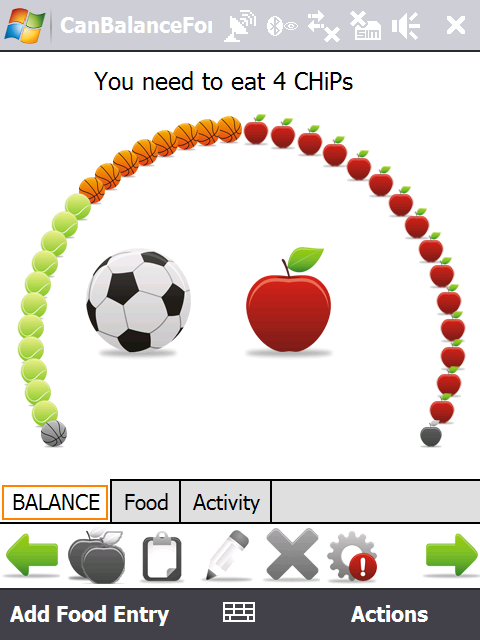
\includegraphics[width=1.25in]{./images/cont1/fig11a}}
		\caption{The home screen with the BALANCE visualization. The orange basketballs indicate CHIPs expended due to BMR. The green tennis balls indicate CHIPs expended due to activity.}\label{fig:fig11a}
	\end{subfigure}
\quad
\begin{subfigure}[t]{1.25in}
		\centering
		\setlength\fboxsep{0pt}
\setlength\fboxrule{0.5pt}
\fbox{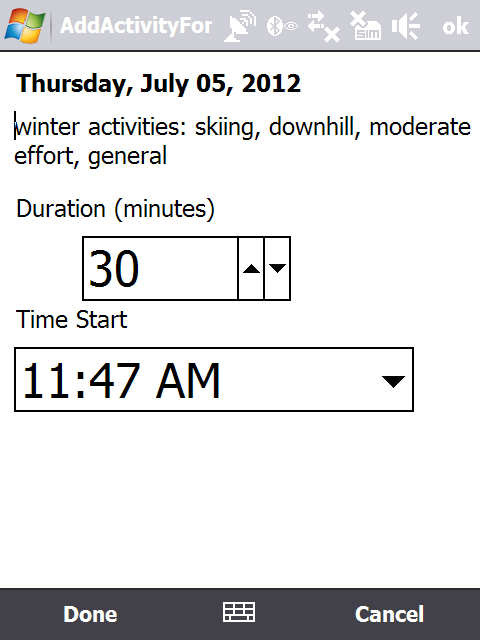
\includegraphics[width=1.25in]{./images/cont1/fig11b}}
		\caption{Adding a physical activity to the diary. The MSB is unable to detect some activities. }\label{fig:fig11b}
	\end{subfigure}
\quad
\begin{subfigure}[t]{1.25in}
		\centering
		\setlength\fboxsep{0pt}
\setlength\fboxrule{0.5pt}
\fbox{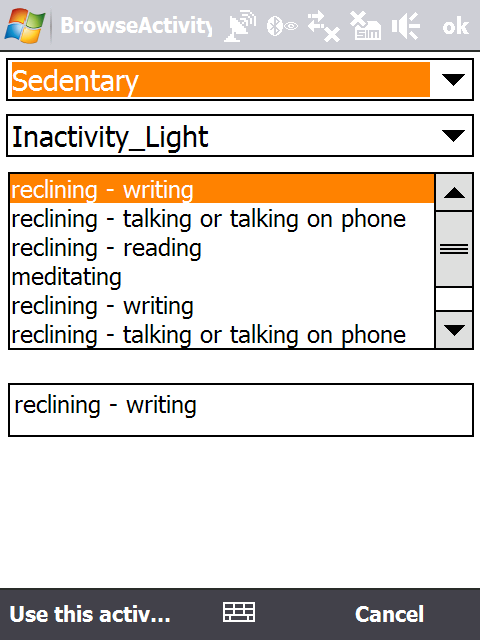
\includegraphics[width=1.25in]{./images/cont1/fig11c}}
		\caption{The list of non-MSB physical activities entered for today.  }\label{fig:fig11c}
	\end{subfigure}
\quad
\begin{subfigure}[t]{1.25in}
		\centering
		\setlength\fboxsep{0pt}
\setlength\fboxrule{0.5pt}
\fbox{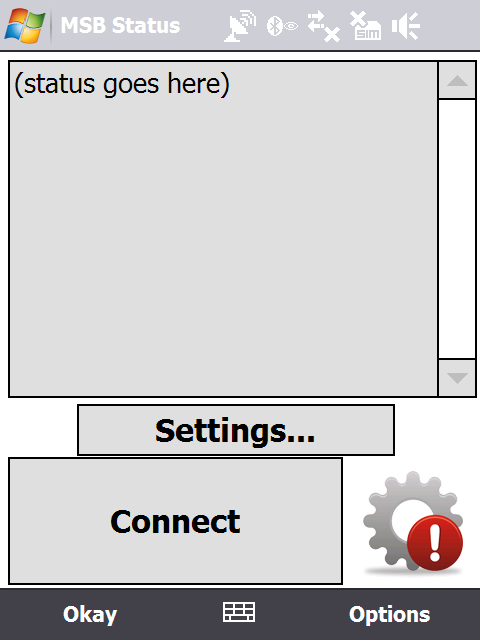
\includegraphics[width=1.25in]{./images/cont1/fig11d}}
		\caption{MSB status and information. }\label{fig:fig11d}
	\end{subfigure}

	\caption{Final BALANCE non-food diary screens.}\label{fig:fig11}
\end{figure}


The pager-sized MSB is worn on the user's hip. It is connected to the phone via a wireless Bluetooth connection. The interface supports connecting to and communicating with the device, displaying information about the sensed activities. The software also monitors the connection and notifies the user if the connection breaks. 


\subsection{24-hr recall software. }
A 24-hr recall is a process in which a trained researcher works with an individual to identify all the foods that the person ate in the past 24 hrs. The protocol is designed to elicit complete and correct dietary intake over the previous 24 hours. The BALANCE validation compared the results from a 24-hr recall to the entries in the mobile phone food diary. This process required a tool for the researcher to access the same food database using the same query process as the BALANCE food diary. We developed a desktop version of the food diary app to support this task. 

\begin{figure}[ t ]
\begin{center}

\setlength\fboxsep{0pt}
\setlength\fboxrule{0.5pt}
\fbox{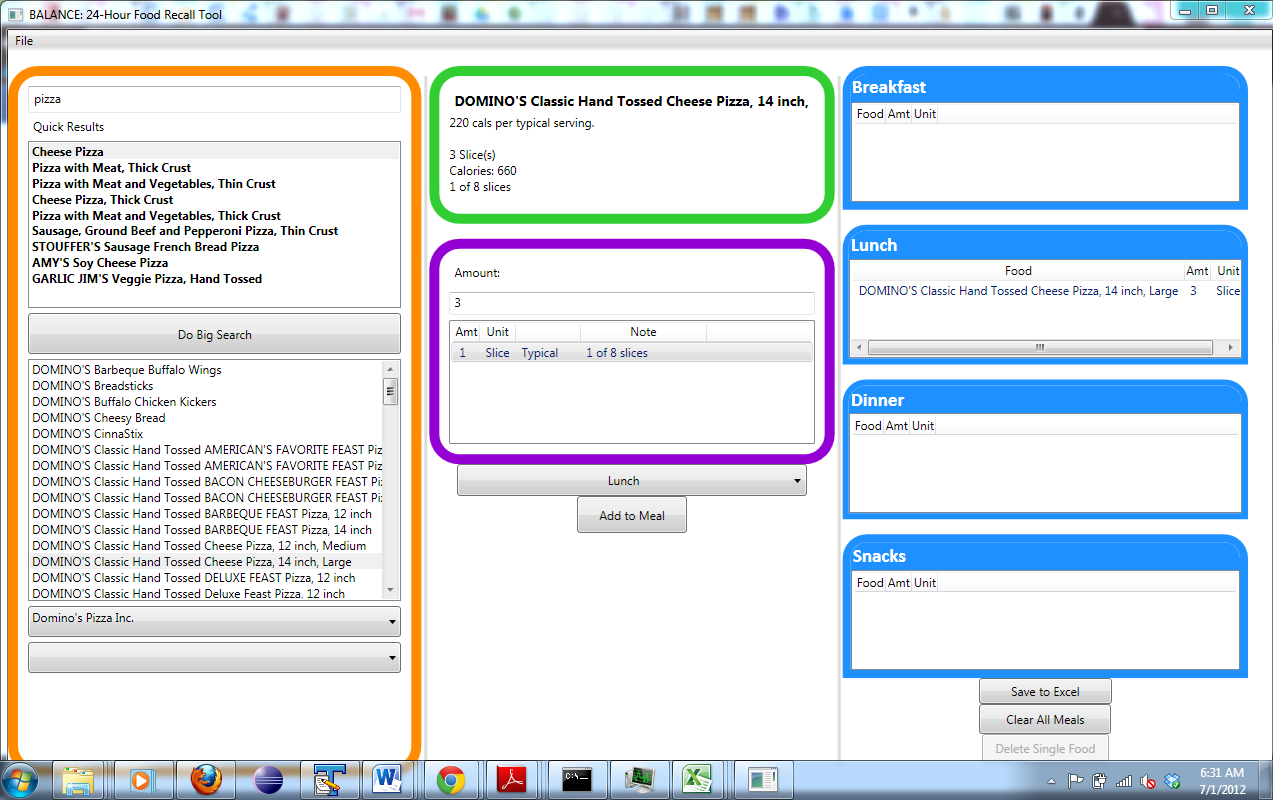
\includegraphics[ width =5.5in ]{./images/cont1/fig12}}

\caption{Software to support the 24-hr recall using the same database and queries as the mobile software.  }
\label{fig:fig12}

\end{center}
\end{figure}

The recall software is pictured in \ref{fig:fig12}. The recall administrator searches for the food in the left pane. The `Quick Results' at the top displays the same foods that the BALANCE mobile user would initially see when searching for a food. The bottom pane allows the administrator to probe about specific manufacturers. The middle pane provides details on a single food and allows amounts to be specified. The right pane shows the foods that have been entered for each meal. The final recall data can be exported to Excel for analysis. 

\subsection{Metrics}
For the evaluation of the focus group-based iterative design process, we defined one measure of interest to be the time between when a food was eaten and when it was entered into the food diary. We found this to be problematic for two reasons: First, participants reported preferring to make entries at the end of the day, regardless of when they ate; second, it relied on participants correctly entering the time that a food was eaten as part of the food entry. As reported in \citet{hughes_balance_2010}, not enough participants modified the time that a food was eaten to make this a useful measure. This led us to consider if other measures could better reflect use of the food diary. Therefore, a secondary goal of this validation phase was to collect data to generate multiple metrics. 

The HCI and Persuasive Technology research communities recognize the potential value of metrics that reflect more details about the use of food diaries. Researchers working in the space of health and wellness have long acknowledged that actual behavior change cannot be the primary measure of success for evaluating tools to help support behavior change \citep{klasnja_how_2011}. Early prototypes and investigations into the space need other measures to indicate whether the tool is developing in the right direction or not. In this vein, researchers are increasingly focusing on \textit{indicators of engagement}, which, loosely defined, are metrics that reflect how engaged an individual is with a particular tool. The reasoning is that the higher the level of engagement (and the more sustained the engagement), the greater the chance for behavior change. However, the usefulness of different indicators of engagement is unclear. 

Additional details about the BALANCE validation study are reported in Snively (\citep{snively_balance_2010}). There, in regards to the food diary, she reports on the overall calories entered into the food diary, the calories reported on the food recall, and analyzes discrepancies. She reports feedback on the usability of the software, but does not report on metrics that indicate patterns of use of the BALANCE food diary. 

In this section, I describe the data that was collected, the metrics that were generated, and report on how well they reflect how the software was used. I also address how these metrics could help interpret the final validation results, which identified a discrepancy between calories entered into the food diary and calories determined via the 24-hr recall. 

\subsubsection{Overview}
As described in Chapter \ref{cha:relatedWork}, previous work reports summary measures of food diary use. These reported measures are usually means reflecting the entire study period. In the rest of this section, I provide more detail, but here I present a quick overview. 

Table \ref{tab:balMetricMeans} reports the means for the four metrics. Days 1-4 reflect active participation in the study. I also include data about Day 5. We found relevant and potentially significant use of the food diary on Day 5, which is technically outside of the study period. 

% Table generated by Excel2LaTeX from sheet 'cont1_meanStartsPerDay'
\begin{table}[htbp]
  \centering
  \caption{Means per participant, per day.}
    \begin{tabular}{lll}
    \toprule
          & Days 1-4 & Days 1-5 \\
    \midrule
    Number of times the software is started & 2.7   & 2.3 \\
    Number of entries created & 9.5   & 8.42 \\
    Number of foods eaten & 9.67  & 8.2 \\
    Number of record edits & 3.02  & 2.97 \\
    \bottomrule
    \end{tabular}%
  \label{tab:balMetricMeans}%
\end{table}%

The means presented above provide a summary understanding of the use of the BALANCE food diary. To further characterize patterns of use over time, each study day is broken into six 4-hr periods, summarized in Table \ref{tab:studyDayTimePeriods}. No distinction is made between weekends and weekdays. These time periods are used for the more detailed analysis in this section. 

% Table generated by Excel2LaTeX from sheet 'Sheet1'
\begin{table}[htbp]
  \centering
  \caption{Add caption}
    \begin{tabular}{ll}
    \toprule
    \textbf{Time frame} & \textbf{Hours} \\
    \midrule
    Early Morning & 12am-4am \\
    Morning & 4am-8am \\
    Late Morning & 8am-12pm \\
    Afternoon & 12pm-4pm \\
    Evening & 4pm-8pm \\
    Night & 8pm-12am \\
    \bottomrule
    \end{tabular}%
  \label{tab:studyDayTimePeriods}%
\end{table}%


\subsubsection{App starts over time}
We start by looking at how often the BALANCE app is started over the course of the study period. Starting the app usually indicates that the user is thinking about the app. In the case of the BALANCE software, starting the app could reflect that the user just ate and is planning to make an entry; is planning to eat and looking up an CHIP values; is glancing at the visualization to assess progress in the middle of the day; or is planning to enter a forgotten entry from earlier in the day. 

As discussed in Chapter \ref{cha:relatedWork}, some researchers report the mean number of times the food diary software was started each day. We calculated this by counting the number of times the software was started over the four days of the study, then dividing by four (the number of days in the study). This results in a mean number of app starts per day in the study period of 2.70. However, we saw that many participants (18) started the software and made entries on the fifth day after the study started. The mean number of app starts over five days is 2.3. 

Figure \ref{fig:chartMeanStartsPerDay} shows the mean number of app starts for each day of the study, including Day 5. The standard deviation is shown as error bars. As expected, the amount of use declines over each day. The low mean on Day 2 reflects that participants were not required to enter their food intake that day. 

\begin{figure}[ tbh ]
\begin{center}

\setlength\fboxsep{0pt}
\setlength\fboxrule{0.5pt}
\fbox{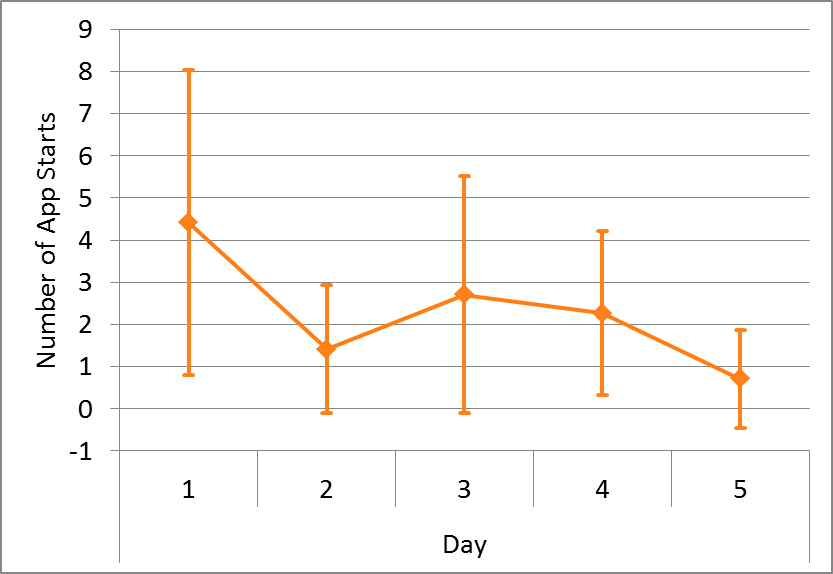
\includegraphics[ width =10cm ]{./images/cont1/chart_meanStarts}}

\caption{Mean app starts for each day. }
\label{fig:chartMeanStartsPerDay}

\end{center}
\end{figure}

One concern we have about reporting the mean number of app starts is its summarizing nature. The mean and standard deviation reflect how much the software was used on each day. However, the BALANCE project is concerned with the distribution of app use throughout a day. The mean does not reflect the relationship between how many times the app was started and how many meals or eating episodes were captured. Participants could start the app repeatedly to enter a single meal, start the app one time for each meal, or start the app one time to enter multiple meals.  

To address this, we calculated how many times the app was started in every 4-hr time period after the start of the study (midnight of Day 1), per participant. The data revealed that some people started the app in multiple time periods; some only started the app within one time period; and some people never started the app. Figure \ref{fig:chart13} reflects how many people reflected each pattern of use. 

\begin{figure}[ tb ]
\begin{center}

\setlength\fboxsep{0pt}
\setlength\fboxrule{0.5pt}
\fbox{\includegraphics[ width =10cm ]{./images/cont1/chart13}}

\caption{App start patterns over the days }
\label{fig:chart13}

\end{center}
\end{figure}


If everyone used the software the way we intended them to, the Figure \ref{fig:chart13} would show 34 people starting the app in multiple time periods (orange) on Days 1, 3, and 4. However, this is not what we see. Consistent with the mean app starts per day, the number of people starting the app in multiple time periods decreased on Days 3 and 4. Inspection of the raw data revealed that 11 people displayed the desired pattern, which indicated that they used the app as requested. 13 people had at least one day (of days 1, 3, or 4) where they did not start the app at all. Five people had two days when they did not start the app at all. Two people started the app one time/day for all four days.

One problem with this calculation is that not starting the app does not always indicate a participant was not using the app consistently throughout the study. Two participants started the app zero times throughout the study period, but still had valid entries. This can be explained that participants treated the phone as a special device used only to enter their food. Since participants were asked to carry a separate device rather than use their personal phone, they were not using the device for anything else. This meant they likely had no reason to ``quit'' and re-start the app. 

\textbf{What does this mean for the validation discrepancy?} This data indicate that for the most part, participants were starting the application periodically through the day. This meant that the discrepancy is probably not due to people forgetting about the application. 

\subsubsection{When entries are made}
Figure \ref{fig:numPeopleEntriesOverTime} shows how many participants created entries during each specified time period. With this population, it was fairly unpopular to make entries in the early morning and morning, while the late morning, afternoon and evening were the most popular times to make entries. 


\begin{figure}[ t ]
\begin{center}

\setlength\fboxsep{0pt}
\setlength\fboxrule{0.5pt}
\fbox{\includegraphics[ width =10cm ]{./images/cont1/chart14}}

\caption{Number of people who made entries in a given time period.}
\label{fig:numPeopleEntriesOverTime}

\end{center}
\end{figure}

\subsubsection{Entry creation time}
This data is generated by counting the number of entries created in a given time period, over the course of the study. This only counts when a record was created in that time period. It does not account for when a food was entered for a different time. This better reflects the pattern of entries that are made throughout the study period, specifically when people are thinking about or using the application. It does not always reflect when people actually ate. 
 
\begin{figure}[ t ]
\begin{center}

\setlength\fboxsep{0pt}
\setlength\fboxrule{0.5pt}
\fbox{\includegraphics[ width =10cm ]{./images/cont1/chart15}}

\caption{Number of entries over time}
\label{fig:chart15}

\end{center}
\end{figure}

This chart shows a sum of all the entries entered during a particular time period each day. While the above chart showed the number of participants who made entries in that time period, this indicates how many entries those participants actually made. 

\textbf{What does this mean for the validation discrepancy?} Reviewing the charts, we see that Day 1 has more people who made more entries earlier in the day. In contrast, on Days 3 and 4 participants made entries primarily in the second half of the day, creating more entries in the second half of the day than in the first half of the day. This indicates that participants were probably entering their food closer to the time that they ate it on Day 1. This implies that the Day 1 entries probably more closely reflects what they actually ate. 

\subsubsection{Food eaten time}

\begin{figure}[ tbh ]
\begin{center}

\setlength\fboxsep{0pt}
\setlength\fboxrule{0.5pt}
\fbox{\includegraphics[ width =10cm ]{./images/cont1/chart16}}

\caption{Number of entries eaten over time.}
\label{fig:chart16}

\end{center}
\end{figure}

Figure \ref{fig:chart16} shows how many valid food entries were reported as being eaten in the given time period, independent of when they were created. 


A comparison of \ref{fig:chart15} and \ref{fig:chart16} indicates that participants likely made entries in the second half of the day capturing food that they ate in the first half of the day. 

\textbf{What does this mean for the validation discrepancy? }Similar to the entry creation time, usage on days 3 and 4 indicate patterns that correlate to greater error between what was eaten and what was entered. This appears less extreme on day 1, so again, the entries on day 1 probably more closely match what was actually eaten. 


\begin{figure}[ t ]
\begin{center}

\setlength\fboxsep{0pt}
\setlength\fboxrule{0.5pt}
\fbox{\includegraphics[ width =5in ]{./images/cont1/chart15_b}}

\caption{Number of entries entered and created over time}
\label{fig:eatenVersusCreated}

\end{center}
\end{figure}

\begin{figure}[ t ]
\begin{center}

\setlength\fboxsep{0pt}
\setlength\fboxrule{0.5pt}
\fbox{\includegraphics[ width =5in ]{./images/cont1/chart_meanEntriesEaten}}

\caption{Number of entries entered and created over time}
\label{fig:eatenVersusCreatedperDay}

\end{center}
\end{figure}

\subsubsection{Comparing entry creation and food eaten time}
Figure \ref{fig:eatenVersusCreated} shows a comparison of the number of records created versus food entries eaten over time. Day 2 shows that there were more entries created than eaten. Since Day 2 was the day participants did not need to make entries, this probably indicates that participants were filling in entries for Day 1, where there are more entries eaten than created. In Days 3, the eaten and created peaks are offset, again indicating that participants probably used the food diary at night to make entries for food eaten in the late morning. Day 4 also shows that morning, late morning and afternoon had more food entries eaten than entered. In this case, they appear to have been created in the afternoon of Day 5. 

\textbf{What does this mean for the validation discrepancy? }Similar to the entry creation time, usage on days 3 and 4 indicate patterns that correlate to greater error between what was eaten and what was entered. This appears less extreme on day 1, so again, the entries on day 1 probably more closely match what was actually eaten. 

\subsubsection{Entry edits}

\begin{figure}[ t ]
\begin{center}

\setlength\fboxsep{0pt}
\setlength\fboxrule{0.5pt}
\fbox{\includegraphics[ width =10cm ]{./images/cont1/chart17}}

\caption{Number of edits over time}
\label{fig:chart17}

\end{center}
\end{figure}


One indicator that users are becoming more familiar and comfortable with a piece of software or an interface is how many errors they make. In this study, the best indication we have for the number of errors people make throughout the whole study is how many edits they make.
 
The mean number of edits made by participants over the entire study is 13.559, with a standard deviation of 8.33. 

Figure \ref{fig:chart17} shows how many edits were made each day of the study, by all of the participants. The decrease in edits over time could indicate that participants were becoming more comfortable with the software, and making fewer errors in their entries. The increase on day 5 could reflect participants checking their entries to prepare for the completion of the study. 

\textbf{What does this mean for the validation discrepancy? }The high number of edits on day 1 could indicate that participants were being conscientious about ensuring that the records were correct. 

\subsubsection{Number Of Combos/Favorites And Their Use}
One of the features asked for many times in the focus groups the ability to save and use favorite foods, combinations, and recipes. In the validation study, 2 participants created 2 combos total, and used one of the combinations 2 times in their diary. 


\subsubsection{Putting it all together }
So far, this section has described metrics that attempt to characterize the use of the food diary over the duration of the study. Now, I will show how the overviews reflect the usage patterns of an individual participant. I will show the details of two participant. The first has the distinction of being one of the participants who did not ever start or quit the application, but otherwise used the food diary as expected. The second participant showed a slightly different pattern of use. 

\begin{figure}[ tb ]
\begin{center}

\setlength\fboxsep{0pt}
\setlength\fboxrule{0.5pt}
\fbox{\includegraphics[ width =5.5in ]{./images/cont1/chart18}}

\caption{All measures, Participant 101}
\label{fig:chart18}

\end{center}
\end{figure}

Figure \ref{fig:chart18} shows all of the measures for Participant 101. This participant showed a decent amount of food diary activity for Days 1, 3, and 4, which is what is expected for this study. However, this is one of the participants who left the software running the entire time. Therefore, no app starts were detected.  On Day 1, in the morning, more foods were eaten than entered, but in the afternoon more foods were entered than eaten. This shows that the participant entered some of the food eaten in the morning, but later in the day went back and added some more entries. On Day 3, the participant was consistent about entering entries when the food was eaten. On Day 4, many more entries were eaten in the afternoon and evening than were entered. On Day 5, some more entries were made, which explains that the participant went back and filled those entries in. 

\begin{figure}[ t ]
\begin{center}

\setlength\fboxsep{0pt}
\setlength\fboxrule{0.5pt}
\fbox{\includegraphics[ width =5.5in ]{./images/cont1/chart19}}

\caption{Patterns of use, ppt120}
\label{fig:chart19}

\end{center}
\end{figure}

Figure \ref{fig:chart19} shows the details for Participant 120. Overall, this participant shows a more consistent interaction with the food diary. The app is started for each time period that we have data. For the most part, entries are entered at the time of eating, with a few edits. Day 1 shows more interaction with the software, which is consistent with a period of adjusting to it. Also, while there are many edits the first day, there are fewer edits in later days, which could indicate a greater familiarity with the software. Starting the app on Day 6 could reflect the participant starting the software to show the study administrator. Day 3 shows that the participant created more entries early in the day, but ate more entries later in the day. This could indicate a planning behavior on behalf of the participant. 

\subsection{Discussion }
In this section, we reviewed metrics that reflected how participants used the food diary in the BALANCE validation. We looked at how and when participants started the food diary app, created entries, reported food as being eaten, and made edits. Participants appeared to start the app more and make more edits on the first day of the study, but the number of entries created and foods eaten were consistent on all three days of the study. This reflects that participants were becoming familiar with the software on the first day. 

The measures show interaction with the software on Days 2 and 5. Day 2 is when participants were not supposed to enter their food, while Day 5 was the day after the study period. The interaction on those days showed that some participants were filling in earlier entries. We also saw that with participant 120, some participants likely used the software to plan ahead, by making entries that reflect being eaten later in the day. 

For this validation phase of the BALANCE study, we chose to present a more detailed treatment of the collected measures due to our experience with the focus group evaluation. In the focus group evaluation, the measure we were interested in was the time between when a food was eaten and when the food entry was created. This measure was not meaningful because too few participants entered the food eaten time when creating the food entries. However, in this validation study, we see evidence that participants did modify food eaten times. There are two potential explanations for this discrepancy. First is that the software was modified throughout the focus group evaluations, and before this final validation. The process to modify a food eaten time may have improved enough to make it easier for participants to modify the entries to reflect the time it was actually eaten. Second, the small sample sizes in the focus groups could impact the effectiveness of the measure. While the validation study does show that participants modified food entries, we also see that some participants probably did not modify the food eaten time. One or two people in each focus group not modifying the food eaten time would impact the quality of that data. 

Previous research has identified factors that increase error in food diaries that people create. In the BALANCE validation study, we identified a discrepancy between what they entered and what was reported in a 24-hr recall. Previous work comparing food entries in an electronic food diary to a 24-hr recall found no significant difference (\citep{glanz_improving_2006}), but one difference between that study and this is that the 24-hr recall was performed a few days into a long-term study, rather than on the first day of a 3-day study. This raises two questions: whether participants were not as familiar with the software and device on the first day, and if the discrepancy may improve if the comparison was performed on the third or fourth day. However, the patterns of use in this study reveal that the Day 1 of the study was probably the most complete food diary data. 

\section{Overall Discussion}
The BALANCE project provides a rich dataset for us to begin understanding some of the challenges that people encounter when trying to self-monitor their food intake on mobile phones. Over the course of our four studies, almost 50 people used the food diary for 3 days and provided detailed feedback. We collected usage metrics of 34 of those participants. These metrics helped us to better understand some of the patterns of use. All of this data also helped us to better understand how our metrics and methodology impacted the evaluation outcomes. I further elaborate on specific themes below. 

\textbf{Historical Context. } The changing technical capabilities of mobile phones were an issue for this project. The BALANCE project began in 2008. Nokia N80s, considered state-of-the-art at the time, were the first devices running the prototype software. These were soon replaced by Nokia N95s. N95s had a larger screens and better technical capabilities overall. The focus group evaluation started in early spring 2009 and finished in late fall of 2009. The validation phase began in spring 2010 and finished in the fall of 2010.

At the beginning of the project, PDAs had been commercially available for more than 10 years, but smartphones were still considered high-end, early adopter technology. Up until that point, both smartphones and PDAs were increasing in capability, but consumers had to choose between the two. However, smartphones were just beginning to merge with PDAs. When this happened, smartphones with touch screens became accessible for consumers. 

Altogether, when we began this project, most people were not using their phone for much more than a basic phone. This was the case even for people with more capable smartphones or PDAs. However, they increasingly aware of the notion of using ``apps'' on a phone. 

\textbf{Fast-changing Technology. } The phone we provided for participants in the focus groups (the WinMobile-based HTC Fuze) was considered `very cool'. One notable comment from a participant was that her teenage son thought she was lucky to be able to use that phone. However, by the end of the project, comments from participants included ``the phone is so clunky and slow''. Indeed, one challenge we have going forward is that it is not likely to be the same phone model as the existing research that has been done. Changing technology platforms throughout a research project introduces challenges for the researchers, but not keeping up with consumer expectations could impact their impressions and feedback of the tool. 

\textbf{Personal Devices.} Administering studies using mobile phones requires researchers to choose whether participants should carry a dedicated study device or if the study software should be installed on a participant's personal device.    \citet{consolvo_conducting_2007} indicate the latter case may be preferable because the participants are familiar with the device and have all of their contact and other personal data on it, therefore may be more likely to use the software on a regular basis. However, study prototypes may be unstable, causing the phone to crash or otherwise interfere with the normal functioning of the phone. In the case of a study-provided device, the participant may be unfamiliar with the device, or have to carry two devices, which may make them less likely to use the software. 

In the BALANCE studies, we chose to provide study-owned devices to the participants to use in addition to their personal phones because of the technical requirements of the project. This could have impacted participant ability to adopt the software readily. The validation study showed evidence that some participants did not start and stop the software as expected. 

\textbf{User Expectations and Research Goals.} 
We had two interim goals as part of the BALANCE project. One goal was to incorporate user feedback to inform the design of the BALANCE software. The other goal was to use the software to collect data to evaluate hypotheses about how the technology supports people tracking their energy intake and expenditure. 


\textbf{User Expectations. }
Researchers developing mobile applications face similar conflicting priorities as developers in a commercial setting.  Putting software into the hands of real users is the best way to help the researcher determine how the software will really be used, what its best and worst features are, and what bugs require repair most urgently. Yet at the same time, users are often intolerant of buggy software and unable to report much more than "it didn't work" as a bug report. As a compromise, we use an iterative approach,  incorporating feedback after each version, and informing testers to the greatest extent possible about the status of the software and procedures for bug reporting.


\textbf{Database. }The food database had a huge impact on the overall design and implementation of the BALANCE software. There was a tension between needing a database that was big enough to have all the foods that many different people may encounter, but small enough to make it quick and easy to navigate. The information architecture of the database was important too-food groups and categories that are meaningful to experts and professionals may not be obvious to consumers. This is consistent with reports of the importance of high literacy abilities to navigate food and nutrition information \citet{rothman_patient_2006}. 

\textbf{Study Duration. }Choosing the duration of the final validation study required evaluating a tradeoff. A shorter duration reduces the burden on the participant. However, a longer duration provides more opportunity for the participant to adapt their routine to incorporate the self-monitoring, while also tailoring the software to reduce the burden. The personal database grows based on what people enter, making it easier to find and enter food. The favorites features also provide a way to minimize interaction time. The three day duration will not merit the time investment required for personalization, and overall will probably not have a large impact on the tracking process. 

The evaluations indicated that people found it challenging to use the BALANCE software to self-monitor food intake in a timely, complete and consistent manner throughout a day. This is consistent with other work that indicated technical malfunction prevented statistically significant results [ref]. Participants reported that the idea of tracking their food intake on their mobile phone was appealing, and offered valuable insight as to how we as designers and researchers may improve the process, particularly by reducing the amount of effort that goes in to the food intake capture. This allows us to raise the question of whether people will be able to enter food intake on a consistent basis if we reduce the amount of effort, in terms of time, physical entry (entering text or pushing buttons) and mental activity (how much the user needs to think about the process). This is addressed in the next chapter. 

\section{Summary}
In this chapter, I describe the BALANCE project, focusing primarily on the design and development of the food diary component of the project. I also provide an HCI-oriented evaluation of the use of the BALANCE software by participants in-situ, to better understand the results of the more quantitative, [medical]-oriented evaluation. This evaluation identified that one important barrier to participants creating complete, comprehensive and timely food entries is due to the database. I document the challenges of using a food database on resource-constrained devices such as mobile phones, and illustrate the inherent challenge of interacting with food databases.  The database is challenging to navigate and requires mental effort, particularly in real-world context, in addition to requiring time-consuming text entry. User feedback indicated that people understand the value that dietary self-monitoring could provide, but that the BALANCE food diary required too much time. It also indicated that people might be willing to accept a less detailed accounting of their food intake in exchange for a less challenging and time-intensive collection process. 

 

% ========== Chapter 2
 \chapter{Investigating Food Index-Based Food Diaries In The Lab}
\label{cha:cont2}
 
In this chapter, I explore challenges around self-monitoring dietary intake without a database on a mobile phone. In earlier chapters, I described the challenges and barriers that people face when employing a traditional approach to journaling what they eat, either on paper, a computer, or a mobile device. This project considers a different approach to the design of a food diary. Specifically, I begin to investigate how recording different information impacts the process of self-monitoring dietary intake. I defer to the constraints that a mobile platform imposes on the self-monitoring of intake problem as discussed earlier, and consider how the use of food indexes could address the given constraints. I also describe how the use of food indexes for mobile phone food journaling naturally reflects known guidelines for supporting successful goal-tending. After providing a theoretical grounding of the approach, I address practical concerns  of using food indexes for mobile phone food diary. I then describe a study where I explore some of those issues and present the results. 

\section{Introduction}
The BALANCE project highlighted the challenges of self-monitoring dietary intake on a mobile device. Many of the challenges were either directly or indirectly related to finding foods in a database. This led us to consider the problem of self-monitoring dietary intake without the database, believing this could help to streamline the food intake capture process. Tinker et al \cite{tinker_measurement_2001} discuss the potential benefits and drawbacks of ``brief'' self-monitoring instruments, pointing out three examples \citep{mossavar-rahmani_additional_2004,Roy1997, Mitchell1996} of previous work that compare the outcomes of brief survey versus detailed self-monitoring tools. \textit{Detailed survey} refers to food diaries that capture all details of an eating episode, including all foods, detailed serving sizes, and time of eating. They could also capture additional context such as location or other people. \textit{Brief survey} tools are designed to capture a fewer details of eating episodes. In the case of Tinker et al, the brief instrument was a `fat scan'. The fat scan is a single piece of paper designed to help users identify and monitor sources of fat in their diet. In addition to the paper-based instruments designed and evaluated above, Mattila et al \citep{mattila_mobile_2008} have used this brief approach to monitoring food intake on a mobile phone. However, this has not been compared to a detailed dietary intake monitoring tool. 

To inform the design of a new brief survey tool, we first considered the larger goal of the BALANCE project, which was to help people self-monitor their energy intake and expenditure to help either attain or maintain a certain weight. Self-monitoring is a tool to help support behavior change, in this case, around health and wellness behaviors. Self-monitoring helps people become aware of their current behavior. Continued self-monitoring helps to identify if the behavior is changing or not. This is related to goal setting and tending--- once awareness is developed via self-monitoring, one can begin to start defining targets for change. Defining goals raises the question of what kind of behavior change we can support without a food database.  A tool can not easily support calorie counting without a database for lookup. However, researchers are interested in other health and wellness indicators such as the quality of an individual diet. 

Diet quality is a factor in preventing and treating many diseases, such as cancer \citep{WHO_CVD_2011}, cardiovascular disease \citep{guh_incidence_2009}, and diabetes \citep{Hu2001}. Research has also shown that a diet high in nutrient dense food tends to be lower in calories \citep{Gibson2000, Cox2000}. Tools to support people in improving their diet quality, especially by increasing the amount of nutrient dense foods they consume, can help them to decrease the number of calories they consume. 

Diet quality is usually measured as a reflection of the pattern of food that an individual consumes, as opposed to values of specific nutrients \citep{kant_indexes_1996, kourlaba_dietary_2009,panagiotakos_adherence_2007}. Different patterns reflect different values of food pattern quality. For example, two dietary patterns commonly referred to include the Standard American Diet (SAD), which reflects how many Americans eat, and the Mediterranean dietary pattern (MedDiet), which reflects traditional eating practices in the Mediterranean. Diet quality is measured and evaluated is through the use of a food index. Food indexes usually consist of a number of components that are scored and then combined together to one overall score. Improving any of the component scores improves the overall score. Food indexes are thoroughly evaluated to ensure that they accurately represent a given diet. Further research investigates the correlation between a given food index and incidence of disease. 

Traditionally, food indexes have been used by experts to evaluate the diet quality of an overall population. Researchers take a form of food intake records (e.g. 24-hr recall, food frequency questionnaire), then calculate the components and overall score according to a set of rules. The report of the food index scores can be used to compare different populations (for example, men versus women in a particular geographic area), compare the change in diet quality over time, or identify areas where certain populations can improve their dietary intake. 

In the absence of a database, food indexes could be a good tool for individuals to track their dietary intake. However, food indexes were developed to be used by experts, and it is unclear what difficulties individuals will have in using them to characterize real food. 

In this chapter, I address the questions of how individuals can use food indexes to directly track their dietary pattern and quality, if there is a benefit in terms of reduced time to make an entry, how correct entries are, and if there is any perceived benefit to the users. 

\section{Food Indexes: Analyzing Diet Quality}
Dietary or food indexes are designed to describe the quality of the diet that a person or population consumes. An index has multiple components, which are weighted and scored differently, then combined to result in one overall number that describes an individual's diet. Research in the nutrition, epidemiological and medical fields correlate the value of different indexes to health outcomes, such as reduced incidence of cardiovascular disease, cancer, or simply mortality \citep{kant_dietary_2010,kant_dietary_2004,kuczmarski_higher_2010}. This makes them appropriate for consideration as a tool to support disease prevention. 

Traditionally, food indexes are used to understand the diet quality of a population as opposed to an individual. An index definition is usually comprised of multiple components and target consumption amounts. Components are either to be moderated (e.g., to place an improved score on consuming less) or attained (e.g., to eat at least a certain amount). Components are based on food groups (fruits, vegetables, grains) or nutrients (sodium, fat, protein) \citep{arvaniti_healthy_2008}. 
There are three basic groups of indexes, based on how they are created: those based on recommended dietary intake of micro- and macro-nutrients (calories, fat, protein, Vitamin A, sodium, fiber), an idealized or preferred dietary pattern (such as the Mediterranean diet), and food groups. An index based on recommended dietary intake uses nutrition databases to determine the macro-and micro-nutrients in each food eaten, and then generates a score via a formula. Indexes or scores based on an idealized pattern focuses more on the kinds of decisions people make about what they eat: choosing lean meats over fatty meats, and olive oil in place of butter. Finally, indexes based on food groups count how many servings of each food group is consumed. Overall, food indexes are discriminate between a diet full of nutrient dense foods and diets high in calorie-dense, nutrient-poor foods. 

An index is used by taking a traditional food journal that consists of a specific food eaten. For discussion purposes, I will refer to a cheeseburger as the specific food.  The researcher will code the food in terms of the food index components. With a food group-based index, the cheeseburger might be coded as ``2 servings of grains (the bun), 1 serving of meat (the patty), 1 dairy serving (the cheese)''. Once the coding is done, an overall score is generated based on a formula accounting for how each component should fit into the larger diet. Scores are sometimes averaged together over populations, which allows researchers to more easily compare or summarize food intake of a large number of people. 

For the purposes of this study, we have identified food indexes that are representative of the different types of food indexes. They are the Healthy Eating Index-2005 (HEI) \citep{guenther_development_2008, guenther_evaluation_2008} and the Food Based Quality Index (FBQI) \citep{lowik_food-based_1999}. The HEI is based on food groups and nutrient amounts, while the FBQI is based only on food groups. We felt it important to choose two indexes that embodied these characteristics for the purposes of exploring how these types of indexes appeal to users. We are choosing to not use an index based on the Mediterranean diet. An index based on an idealized dietary pattern assumes that the user has previously committed to a particular diet philosophy. 

\subsection{Food Indexes and Goal Setting}
\citep{consolvo_goal-setting_2009, cullen_using_2001,dewalt_goal_2009,intille_just--time_2003,locke_building_2002,shilts_goal_2004}

\subsection{The Healthy Eating Index-2005 }
The Healthy Eating Index (HEI) \citep{guenther_development_2008, guenther_evaluation_2008, kennedy_healthy_1995} is a food index based on the USDA Dietary Guidelines for Americans \citep{us_health_and_human_services_dietary_2005}. The original HEI was developed in 1995 and revised in 2006 to reflect the 2005 Dietary Guidelines. Throughout the rest of this document, the acronym `HEI' refers to the 2005 version of the HEI. 

The HEI is a score based system, with a high quality diet obtaining a score of 100 points. Each of 12 components contribute to the overall score. Table \ref{tab:table2_1} lists the components and their individual contribution to the overall score. The components above the line are attainment components. Researchers want people to eat more of these components. The attainment components for HEI contain primarily food groups. Components below the line are moderation components. Researchers recommend reducing or restricting the consumption of these components. All of these components are considered nutrients. The scoring of the attainment and moderation components reflect that most Americans do not eat enough of certain food groups (dark green and orange vegetables, whole grains) and consume too much of certain nutrients (sugar, saturated fat, calories). The calculation for each point depends on the individual daily recommended caloric intake.

% Table generated by Excel2LaTeX from sheet 'Sheet3'
\begin{table}[tbhp]
  \centering
  \caption[HEI Calculation.]{The HEI calculation. A close-to-perfect diet will score 100 points. Points are defined in regards to the recommended number of calories an individual should consume. Components above the line are attainment. Components below the line are moderation.}
    \begin{tabular}{p{2in}cl}
    \toprule
    \textbf{Component} & \textbf{Maximum Points} & \textbf{Daily Recommended Intake} \\
    \midrule
    Total Grains & 5     & $\ge$ 3.0 oz eq/1000 kcal \\
    Whole Grains & 5     & $\ge$ 1.5 oz eq/1000 kcal \\
    Vegetables & 5     & $\ge$ 1.1 cup eq/1000 kcal \\
    Dark green \& orange vegetables, legumes & 5     & $\ge$ 0.4 cup eq/1000 kcal \\
    Total Fruits & 5     & $\ge$ 0.8 cup eq/1000 kcal \\
    Whole Fruits & 5     & $\ge$ 0.4 cup eq/1000 kcal \\
    Milk  & 10    & $\ge$ 1.3 cup eq/1000 kcal \\
    Meat and Beans & 10    & $\ge$ 2.5 oz eq/1000 kcal \\
    Oils  & 10    & $\ge $12 g eq/1000 kcal \\
\hline
    Saturated Fat & 10    &$ \le 7\%  $ of total kcals consumed\\
    Sodium & 10    & $\le $0.7 g/1000 kcal \\
    Calories from Solid Fats, Alcoholic Beverages, and Added Sugars & 20    &   $\le$ 20\% of total kcals consumed \\
\hline\hline
    Total Points & 100   &   \\
    \bottomrule
    \end{tabular}%
  \label{tab:table2_1}%
\end{table}%


Grains, vegetables and fruits are broken into multiple categories. The grains category is separated into Whole and Total grains, as is the Fruit category. For Grains, once the daily limit is met for Whole Grains, more Whole Grains are counted under Total Grains. If a person eats five Whole Grains and five Total Grains, the grains component of the total score is 10. However, if a person eats 10 Total Grains, the grains component of the total score is 5, since none were Whole Grains and the max Total Grains score is 5. This is similar with Fruit, where Whole Fruits include unprocessed fruits, while Total Fruits includes juices and cooked or dried fruits. Vegetables also include two categories, separating out the dark green and orange vegetables, as well as legumes. Similar to Grains and Fruits, if one eats the equivalent of 10 points of Dark Green Vegetables, the total score is 10, while 10 points of other vegetables only contributes 5 points to the total score. 

The rules to calculate an HEI score for an individual diet are fairly complicated. However, partly due to the complexity, researchers find the resulting score a fairly good indicator of one's diet \citep{guenther_evaluation_2008}. The complexity makes it a good option for this study. It will help us to identify user responses to a complex interface and counting process. It also incorporates the restricting some important quantities. 


\subsection{The Food-Based Quality Index}
The Food-Based Quality Index (FBQI) \citep{lowik_food-based_1999} is a food index based solely on food groups. The FBQI food groups are simplified and slightly different than the ones based on the food groups defined by the USDA. Specifically, potatoes, rice, pasta, and other starchy grains are considered separately from either bread (and cereal grains) or vegetables. Cheese is separate from dairy. Serving specifications are designed to be representative of how consumers think about food servings. 

The FBQI is simpler than the HEI: It is based only on food groups with no accounting of nutrients; all components are target rather than attain or moderate; and serving sizes are intended to be user-friendly. However, the familiar serving sizes are vague. The simplicity of the FBQI is a good contrast to the HEI for an initial investigation of using food indexes for self-monitoring dietary intake. 

% Table generated by Excel2LaTeX from sheet 'Sheet4'
\begin{table}[tbhp]
  \centering
  \caption[FBQI Calculation]{FBQI Calculation. Each component accounts for a single point, but the target is a range. All components are targets; there are no attain or moderate components.}
    \begin{tabular}{lll}
    \toprule
    \textbf{Component} & \textbf{Points} & \textbf{Serving goal} \\
    \midrule
    Bread (incl. breakfast cereals) & 1     & 5-7 slices \\
    Potatoes (incl. rice, pasta \& pulses) & 1     & 3-5 pieces \\
    Vegetables & 1     & 3-4 serving spoons \\
    Fruit & 1     & 2 pieces \\
    Milk \& milk products & 1     & 2-3 glasses \\
    Cheese & 1     & 1-2 slices \\
    Meat, fish \& eggs & 1     & 115-130 g \\
    \bottomrule
    \end{tabular}%
  \label{tab:table2_2}%
\end{table}%

 
\section{Food Tasks: Food Diary Evaluation Methodology}
Section \ref{sec:food_task_challenges} details important considerations of choosing how to present food tasks to study participants. Those challenges are primarily how to choose which food to use in the tasks and how to present those foods to the participant. 

There are four options for presenting food tasks to participants: using real food; food models; food photographs; or food names. For practical purposes, we chose to use food names. For each food, the food name presented is from the Food Name field in the Nutritionist Pro KnowledgeBase. 

Food tasks were chosen... 
Concerns for choosing food tasks: 
\begin{itemize*}
\item Familiarity: chose foods from a previous study using the same population. 
\item combination foods: chose a balance of combo/prepared foods and single foods. 
\item amount of foods: used a 2000 kcal diet. 
\item number of foods: specific number of foods per meal. 
\item coverage for FBQI and HEI: chose foods to ensure that most or all components of HEI/FBQI were used in each `day' of food. 
\end{itemize*}


Since familiarity is so important, we carefully considered how to choose the food for the tasks. One considered approach was to refer to a published gold standard. [blah blah, not published, not an issue in nutrition research, etc. ] We considered using published diet plans, such as those advocated by the American Heart Association for healthy diets. The drawback to those is that they are recommended, and may not accurately reflect the actual diet of the participants. Additionally, since the recommended menus are based on the official Food Pyramid, and one chosen food index is also based on the Food Pyramid, this could influence the correctness scores. After consideration, we decided to choose the food tasks based on the food diaries collected in the BALANCE focus groups. Since the study populations are drawn from the same underlying populations, the issue of familiarity is addressed. More details are explained later. 

Another important aspect is how the food tasks are presented to participants. In the real world, one of the important challenges to ``perfect'' food journaling is the process of seeing/eating food, identifying what it is, sometimes identifying methods of preparation (fried versus broiled), identifying un-seen characteristics (low-fat versus full-fat milk, with butter), and identifying portion or serving sizes in order to correctly enter the food (or choose from a list in a db). Sometimes this process is easy, as with packaged foods or when preparing your own food; other times such as at a restaurant it is more challenging. Literacy is also an issue: with a traditional journaling approach, it is one thing to be able to identify one cup of spaghetti, but if you are not able to spell it properly, you might not be able to find it in a database. Due to this process, we considered that using real plates of food would be more life-like, and that using photographs of food were close to real. However, with the use of photographs, care must be taken to obtain them properly. Scale and lighting are two important considerations. And, with research, we found that there exist food photograph booklets specially prepared for the purpose of studying people's estimation of portion sizes. However, these booklets had the familiarity concerns outlined above. We decided that portion size estimation and literacy were not primary concerns for this study, so chose to present food tasks as a list of foods on a card. 

\section{Investigating and Comparing Food Index-Based Mobile Phone Food Diaries}
In this section, I talk about the evaluation I did to explore this area of tracking diet quality or food-index based tracking. 
\subsection{Research Aims}
\begin{enumerate*}
\item Is it faster to enter food in a complete, index-based mobile phone food diary?
\item Are people able to enter food correctly in a complete, index-based mobile phone food diary?
\item Are the work-load satisfaction measures the same for index-based mobile phone food diary as a traditional food diary?
\item How can we characterize the types of errors that are made in an index-based mobile phone food diary?

\end{enumerate*}

In addition to the above research questions, we designed this study to support generating design recommendations for future index-based food diaries. 

\subsection{Study Design}
We performed a comparative evaluation of the BALANCE interface with two food index-based food diaries. The other food diaries were based on HEI and FBQI. All interfaces were ran on a Windows Professional Mobile smartphone with a slide-out, qwerty keyboard. 

\subsection{Instruments}
This study focused primarily on understanding the interaction between people and a food index via a mobile device. 

The BALANCE interface was a modified version of the software for the BALANCE study. The modifications are detailed later. The HEI and FBQI interfaces were designed to be simple, similar, and reflect the food indexes. Both interfaces displayed all of the index components as boxes on the home screen. Daily progress for each component was shown as checks on each box. Each box had a button labeled ``Ex.''. This button opened a dialog window with a short description of the component and some example foods. This example information was intended to help users answer the question ``I just ate a food; which group does it go in?''. The example content was adapted from literature describing the indexes. 

Touching the index component button opens a serving size screen. This screen also provides examples of foods in that component and sample serving sizes. The widget for specifying servings was a set of buttons that could be toggled on and off. The buttons act like a slider: when a multiple-sized entry is made, all the others are selected. That is, clicking the 3 oz button selects the 1, 2, and 3 oz. buttons. 

The HEI and FBQI interfaces went through a paper prototype design process. One design feature explored in particular was the use of images to represent each component. Appropriate images could greatly improve user ability to remember what foods belong in which component. However, inappropriate images could have a large negative impact. Instead, we chose to use colors to represent each component. The same colors represented similar groups in HEI and FBQI, as much as possible. Finally, we designed the layout of the component buttons to all fit on the overview screen with no scrolling. This provided both an easy way to view the overview and make a new entry. 

Guiding Design Principles:
\begin{itemize*}
\item Overview on one screen
\item Overview shows progress but not goals or targets
\item Individual screens inherently showed goals (maximum number of boxes)
\item One handed use
\end{itemize*}


\subsubsection{HEI}
It is straightforward to convert the HEI index into a points-based system that is appropriate for our indexed-based system. For the study, we assumed a daily recommended intake of 2000 kcals. The official recommended intake for healthy adults is roughly 1900-2400 kcals/day. In real-world usage, the interface can reflect an individual's need, but for the study this was fine. We then calculated the recommended intakes for each group. For the interface, we made small adjustments to the amounts to target intakes to make it easier to count ``points''. We then chose a number of boxes to use to represent the points that was fairly straightforward and more human-friendly. For example, we rounded 2.2 cups of vegetables up to 2.5 cups, and presented it as 5 boxes, so that each box represented 0.5 cups of vegetables. This appears friendlier than 5 boxes with each representing 0.44 cups. We edited the ``What's in a serving'' text to reflect the amounts that each box represented. For the Vegetables, Fruits and Grains categories, where there are two sub-categories of foods, we ensured that each box for both sub-categories represented the same amount. For example, in the case of Grains, the target for Whole Grains is 3 oz, while the target for Total Grains is 6 oz. Rather than have 6 boxes for each (which means that the boxes for Whole Grains would represent 0.5 oz while the boxes for Total Grains would represent 1.0oz), we chose to have 3 boxes for Whole Grains and 6 boxes for Total Grains, and each box represents 1 oz. 

For the purposes of this study, we collapsed Fruit, Vegetables and Grains into single categories, each with two sub-categories. We did this to reduce the complexity of the overview screen for two reasons. First was because we wanted the overview screen to contain all of the index components and still be simple, uncluttered, and one-hand usable. Putting three more boxes on the overview screen would make the boxes too small. When the boxes are too small, they're more difficult to target/touch, and also have less space to show the checkmarks that identify current progress/status for the day. The second reason was that we wanted to reduce the cognitive load at the overview level. There are two tasks that we want to support with the overview screen: answering the questions of ``how is my progress so far today?'' and ``Where do I put this food?''. To answer the ``Where do I put this food?'' question, the fewer number of answers that are possible makes it an easier question to answer. For that immediate moment, it is easier (and quicker) for a person to judge ``is this carrot a fruit or a vegetable?''; once they get to the servings dialog, they can address the ``is it orange or not?'' question. 

% Table generated by Excel2LaTeX from sheet 'Sheet3'
\begin{table}[htbp]
  \centering
  \caption{Counting HEI as `tokens'}
    \begin{tabular}{p{2in}lllrl}
    \toprule
    Component & Goal  &       & Num Boxes & Daily Recommended Intake &  \\
    \midrule
    Total Grains & 6 oz  & 6 oz  & 6     & $\ge 3.0 oz eq/1000kcal$ &  \\
    Whole Grains & 3 oz  & 3 oz  & 3     & $\ge 1.5 oz eq/1000kcal$ &  \\
    Vegetables & 2.2 cups & 2.5 cups & 5     & $\ge 1.1 cup eq/1000kcal$ &  \\
    Dark green \& orange vegetables, legumes & 0.8 cups & 1 cup & 2     
& $\ge 0.4 cup eq/1000kcal$ &  \\
    Total Fruits & 1.6 cups & 1.5 cups &       & $\ge 0.8 cup eq/1000kcal$ &  \\
    Whole Fruits & 0.8 cups & 1 cup &       & $\ge 0.4 cup eq/1000kcal$ &  \\
    Milk  & 2.6 cups &       &       & $\ge 1.3 cup eq/1000kcal$ &  \\
    Meat and Beans & 5 oz  & 5 oz  & 5     & $\ge 2.5 oz eq/1000kcal$ &  \\
    Oils  & 24 g  & 25 g  & 5     & $\ge 12 g eq/1000kcal$ &  \\
    Saturated Fat &       & 7.5g  & 5     & $\le 7\%  of energy$ &  \\
    Sodium & 1.4 g &       &       & $\le 0.7 g/1000kcal$ &  \\
    Calories from Solid Fats, Alcoholic Beverages, and Added Sugars &   !!    &       &   !!?    & $\le 20\% of energy$ &  \\
    \bottomrule
    \end{tabular}%
  \label{tab:table2_3}%
\end{table}%



\begin{figure}	
\centering
	\begin{subfigure}[t]{1.25in}
		\centering
		\setlength\fboxsep{0pt}
\setlength\fboxrule{0.5pt}
\fbox{\includegraphics[width=1.25in]{./images/cont2/fig1a}}
		\caption{The main screen. Each block represents an HEI component. }\label{fig:hei_a}
	\end{subfigure}
\quad
\begin{subfigure}[t]{1.25in}
		\centering
		\setlength\fboxsep{0pt}
\setlength\fboxrule{0.5pt}
\fbox{\includegraphics[width=1.25in]{./images/cont2/fig1b}}
		\caption{The `Ex.' button provides guidance on each component.}\label{fig:hei_b}
	\end{subfigure}
\quad
\begin{subfigure}[t]{1.25in}
		\centering
		\setlength\fboxsep{0pt}
\setlength\fboxrule{0.5pt}
\fbox{\includegraphics[width=1.25in]{./images/cont2/fig1c}}
		\caption{Touching a colored component box on the main screen opens a dialog where the user can specify how much of that component was eaten. One block represents a yellow checkmark.  }\label{fig:hei_c}
	\end{subfigure}
\quad
\begin{subfigure}[t]{1.25in}
		\centering
		\setlength\fboxsep{0pt}
\setlength\fboxrule{0.5pt}
\fbox{\includegraphics[width=1.25in]{./images/cont2/fig1d}}
		\caption{The yellow checks represent how much of each component was eaten on the current day. }\label{fig:hei_d}
	\end{subfigure}
	\caption{The HEI interface.}\label{fig:hei_instrument}
\end{figure}



The main screen of this application shows an overview of the index. Each colored button represents a component of the index, labeled as such. An ``Ex'' button on each component button provides support for the user to determine which group/component a particular food belongs to. The ``Ex'' button for Grains is shown above. With HEI, many of the components(Vegetables, Fruits and Grains) are broken down into sub-components. Once a component button is selected, a window pops up which allows a user to specify how many servings they  want to enter. Again, the example/explanatory information is presented on this page, to support the user in determining how many servings to select. For this study, the serving sizes was based on the formal HEI specification. We see in the case of grains, this is ounces of grains. The examples and explanatory guidance text is adapted from information provided by official food pyramid guidance. After the servings are selected, the overview screen shows checkmarks to represent the number of servings eaten in that category, accumulated for the day. 

\subsubsection{FBQI}

The FBQI interface is similar in design to the HEI inteface. This is specifically to attempt to minimize differences between the interfaces. As in HEI, the main screen shows an overview of the index. Each colored button represents a component of the index, labeled as such. An ``Ex'' button on each component button provides support for the user to determine which component a particular food belongs to. The ``Ex'' button for Grains is shown above. Once a component button is selected, a window pops up which allows a user to specify how many servings they  want to enter. Again, the explanatory information is presented on this page, to support the user in determining how many servings to select. The serving sizes and guidance are based on the official definition of the food index. The guidance for the FBQI is more streamlined, which is indicative of the point that the index is designed for experts, as opposed to novices. Consumers may find the simplification beneficial, but sometimes does not provide enough guidance for the various foods people encounter in their diet. The examples and explanatory guidance text is very similar to the guidance provided for HEI, and adapted from USDA food pyramid \citep{us_health_and_human_services_dietary_2005} guidance. After the servings are selected, the overview screen shows checkmarks to represent the number of servings eaten in that category, accumulated for the day. 

\begin{figure}	[tbh]
\centering
	\begin{subfigure}[t]{1.25in}
		\centering
		\setlength\fboxsep{0pt}
\setlength\fboxrule{0.5pt}
\fbox{\includegraphics[width=1.25in]{./images/cont2/fig2a}}
		\caption{The main screen shows a colored box representing each component.  }\label{fig:fbqi_a}
	\end{subfigure}
\quad
\begin{subfigure}[t]{1.25in}
		\centering
		\setlength\fboxsep{0pt}
\setlength\fboxrule{0.5pt}
\fbox{\includegraphics[width=1.25in]{./images/cont2/fig2b}}
		\caption{The `Ex.' button shows guidance for each component.}\label{fig:fbqi_b}
	\end{subfigure}
\quad
\begin{subfigure}[t]{1.25in}
		\centering
		\setlength\fboxsep{0pt}
\setlength\fboxrule{0.5pt}
\fbox{\includegraphics[width=1.25in]{./images/cont2/fig2c}}
		\caption{Touching the colored box opens a dialog where the user can specify how much was eaten. }\label{fig:fbqi_c}
	\end{subfigure}
\quad
\begin{subfigure}[t]{1.25in}
		\centering
		\setlength\fboxsep{0pt}
\setlength\fboxrule{0.5pt}
\fbox{\includegraphics[width=1.25in]{./images/cont2/fig2d}}
		\caption{Yellow checkmarks show how much of each component had been eaten on the current day. }\label{fig:fbqi_d}
	\end{subfigure}
	\caption{The FBQI Interface. }\label{fig:fbqi_interface}
\end{figure}



\subsubsection{BALANCE}
The main, overview screen for the BALANCE software consists of a list of food eaten that day. For each food item, the name, number of calories, and meal is identified. The number of calories for that day is specified at the top of the screen. New entries are added by searching for a key word or name. After 3 letters are entered, a list is displayed that shows food entries (from a list of foods that contain common foods and foods that have been entered by that user before) that contain words starting the same way. After a specific food is chosen, a screen appears where the user can specify the amount eaten, in full and partial servings. Some foods provide multiple serving choices, such as ounces, cups, grams, pieces, or servings. This information is provided by the nutrition database, and is limited to the serving information in this database. 

\begin{figure}	[tbh]
\centering
	\begin{subfigure}[t]{1.25in}
		\centering
		\setlength\fboxsep{0pt}
\setlength\fboxrule{0.5pt}
\fbox{\includegraphics[width=1.25in]{./images/cont2/fig3a}}
		\caption{The modified BALANCE interface. The ``Add Food'' menu was changed to a button. The tool bar only allows editing and deleting food entries. }\label{fig:bal_a}
	\end{subfigure}
\quad
\begin{subfigure}[t]{1.25in}
		\centering
		\setlength\fboxsep{0pt}
\setlength\fboxrule{0.5pt}
\fbox{\includegraphics[width=1.25in]{./images/cont2/fig3b}}
		\caption{Enter the food name to search. }\label{fig:bal_b}
	\end{subfigure}
\quad
\begin{subfigure}[t]{1.25in}
		\centering
		\setlength\fboxsep{0pt}
\setlength\fboxrule{0.5pt}
\fbox{\includegraphics[width=1.25in]{./images/cont2/fig3c}}
		\caption{Specifying the amount eaten. }\label{fig:bal_c}
	\end{subfigure}
\quad
\begin{subfigure}[t]{1.25in}
		\centering
		\setlength\fboxsep{0pt}
\setlength\fboxrule{0.5pt}
\fbox{\includegraphics[width=1.25in]{./images/cont2/fig3d}}
		\caption{The food listed on the main screen. }\label{fig:bal_d}
	\end{subfigure}
	\caption{Modified BALANCE interface. }\label{fig:bal_interface}
\end{figure}



\subsection{Participants}

12 participants, recruited from online campus newspaper. The mean age was 31.6 years, median age 28.5 years; 8 females. 7 participants owned a phone with a touch screen, 5 owned ``feature phones''. Of the 12 subjects, 10 of them reported using their cell phone either daily (1-2 times per day) or several times a day, while 2 reported using their phones approximately 1-2 times per month. 7 reported entering text (such as text messages or adding/modifying contacts) on their phones either daily (1-2 times per day) or several times a day, while 3 enter text approximately 1-2 times per week and 2 almost never enter text on their phones. Of participants who enter text on their phones, 5 use a 12-key keypad; 3 use a touch screen or soft keyboard; and 3 use a QWERTY or hardware keyboard. 

\subsection{Procedure}
Participants came to the lab, and began by filling out a questionnaire that included basic demographic data, questions concerning the participants' daily cell phone use, current health and wellness goals, and experience journaling food intake. 

Then, for each interface, they were introduced to the interface and given two practice tasks to perform. The practice tasks were the same for all interfaces. One practice task consisted of only single foods, and the other practice task consisted of combination foods. After the practice tasks, the participants were given a chance to ask any questions or take a break. They were then notified that the real tasks were starting, and asked to work as quickly as comfortable between the start of a task and the end. 

A task consisted of a meal, which was printed on a card. At the start of each task, the task card was set on the table next to the participant, and phone displayed a screen that identified the coming task (by task ID). This allowed the study administrator to ensure that the correct task was being timed (by comparing the task ID on the screen with the card). When the participant is ready, they click on the ``Start Task'' button, then refer to the task card for entries. When the participant believes the task is complete, they click the ``done'' button. Another screen showed that the task was over. The participant then clicks ``next task'' when they are ready, and the cycle starts again. 
One day of meals was completed in each condition. This consisted of a breakfast, lunch, dinner, small snack, and large snack. After each condition, participants filled out a TLX survey and asked what they like best and least about each condition. The presentation of food days and order of conditions was counterbalanced.

After all three conditions were complete, the participants completed a final survey on the computer. 

\subsection{Tasks}
For each condition, participants have ``food tasks'' for the participants to enter. Food tasks are broken down into ``meals'', and there will be a controlled set of foods in each meal. 

There were 3 days of food tasks. Each day consisted of a breakfast (3 food items), small snack (1 item), lunch (4 items), big snack (2 items), and dinner (6 items). Each day was chosen to control for number of items, number of calories, and number of index components. Foods and meals were chosen from a previous study that collected food journals from a similar population. This ensured that most foods would be recognized and familiar. Specifically, foods were chosen only if they existed in the nutrition diary that BALANCE is based on. This has the benefit that we can more closely compare things like time to enter between conditions, but it is clearly not representative of the real world, where many foods are not included in the database. This is a problem that has proven to be a barrier for many food diaries. 

\subsection{Study Design Limitations}
This study simplifies the food journaling process in order to directly compare the strengths and weaknesses of the interfaces. There are three primary limitations to the design of this study: it does not address the problem of either estimating or measuring serving sizes; none of the tasks include foods that are not in the database; and there is no real-world context. 

\subsection{Data Collected}
The data collected is described in more detail below. Special attention is given to the treatment of how to count task responses as correct. 


\textbf{Duration.} Time spent in each condition. Time was calculated as the sum of time spent in each meal, starting when the ``start'' button was clicked and stopping when the ``done'' button was clicked at the end. Time between meal tasks was not counted. 



\textbf{Correctness.} A value indicating how correct the task response was. A task is assigned 2 points for entirely correct, 1 point for mostly correct, and 0 points for not correct. A participant can get a maximum score of 10 in each condition. Entirely correct means it is exactly ground truth; mostly correct means that there was a small difference that was not entirely correct, but the meaning was close (for example, replacing ``feta'' with ``blue cheese'', or ``Hidden Valley Ranch Dressing'' with ``creamy salad dressing'' in the BALANCE condition). This was done by inspection by the lead researcher. 

This approach to measuring correctness is due to the complexity of comparing errors across conditions. In all three conditions, it was common for users to provide an answer that was close to correct, but not entirely. This approach, in conjunction with a more thorough analysis of the exact errors that were made, allows us to better compare how well participants performed in each interface. 


\textbf{TLX.} Self-reported measure of workload assessment. After each condition, participants filled out a NASA-TLX survey \citep{Hart2006}. Items include Mental Demand, Physical Demand, Temporal Demand, Performance, Effort, and Frustration,  and are rated on a 7-point Likert scale. 

\textbf{Rankings.} Ordering of the interfaces on four features. At the end of the study, participants ranked each interface in terms of preference, ease of use, understandability, and usefulness.

\textbf{Useful for goals.} Self-reported indication of how useful each interface would be to help reach goals. At the end of the study, participants were asked which single interface they felt would be most helpful for them to reach their health and wellness goals, and why. 



\textbf{Length of use.} Self-reported duration a participant would be willing to use the interface for. At the end of the study, participants were asked which interfaces they felt they could use for three days, three weeks, and three months. 

\textbf{Likes and dislikes. } Self-reported features that participants liked or did not like. After each condition, participants were asked to list three things they liked about the previous condition, and three things they did not like.

\textbf{Errors.} Difference between the ideal or expected task response and what the user entered. An error was identified as a difference between a participant food entry (the final ``daily'' entry'') and the expected/perfect entry. This is different than the correctness measure described earlier. Correctness is a score designed to support comparison between conditions. Here, we compare and report on the errors within one condition. 


\subsection{Hypotheses}
Tested hypotheses: 
\begin{enumerate*}
\item Both of the index-based interfaces (HEI and FBQI) will be faster than the BALANCE interface. 
\item The FBQI interface will have more errors than the BALANCE interface; HEI interface will have more errors than the FBQI interface.  
\item The TLX workload measures will be the same for all three interfaces. 
\end{enumerate*}

Can we begin to characterize the types of errors that are made in a complete, index-based mobile phone food diary? 


\subsection{Data Analysis and Results}
Since this work was an early exploration, we performed both quantitative and qualitative analyses. The quantitative analysis focused on comparing performance of the interfaces. The qualitative analysis focused on proving insight into the use of the food indexes for self-monitoring of dietary intake. This included a thematic analysis of the answers provided to the self-report questions, an analysis of the errors made in each condition, and a discussion of the answers to the question ``Which interface will help you reach your health and wellness goals?''


% Table generated by Excel2LaTeX from sheet 'Sheet5'
\begin{table}[htbp]
\tiny
  \centering
  \caption{Summary of statistical analyses}
    \begin{tabular}{lp{1.5in}cp{2.5in}}
    \toprule
    Measure & Test  & Significance & Values to report \\
    \midrule
    \textbf{Correctness}\footnote[1]{Significant}
 & 1-way repeated measures ANOVA & Y     & ($F_{2,22}=17.074, p<0.0001$). \\
    \textbf{} & Paired t-test & Y     &  \\
    \textbf{Duration}$^{a}$ & 1-way repeated measures ANOVA & Y     & (Wilks� lambda $= 0.154, F_{2,10}=27.49, p<0.0001$). \\
    \textbf{} & Paired t-test & Y     &  \\
\midrule
    \textbf{TLX: } &       &       &  \\
    \multirow{2}[0]{*}{\textbf{Mental Demand}} & \multirow{2}[0]{*}{Friedman test} & \multirow{2}[0]{*}{Y} & \multirow{2}[0]{*}{ ($\chi^2=10.56, N=12, df=2, p<0.01$).} \\
          &       &       &  \\
    \textbf{} & Wilcoxon & N     & With Bonferroni correction, no pair-wise comparisons are significant.  \\
    \textbf{Discouraged} & Friedman & N     & ($\chi^2=2.595, N=12, df=2, p=0.273$). \\
    \multirow{2}[0]{*}{\textbf{Ease of use}} & \multirow{2}[0]{*}{Friedman} & \multirow{2}[0]{*}{N} & \multirow{2}[0]{*}{($\chi^2=3.556, N=12, df=2, p=0.169$).} \\
          &       &       &  \\
    \multirow{2}[0]{*}{\textbf{Quickly}} & \multirow{2}[0]{*}{Friedman} & \multirow{2}[0]{*}{N} & \multirow{2}[0]{*}{($\chi^2=1.333, N=12, df=2, p=0.513$).} \\
          &       &       &  \\
    \textbf{Learn} & Friedman & N     & ($\chi^2=0.963, N=12, df=2, p<0.618$). \\
    \multirow{2}[0]{*}{\textbf{Successful}$^{a}$} & \multirow{2}[0]{*}{Friedman} & \multirow{2}[0]{*}{Y} & \multirow{2}[0]{*}{ ($\chi^2=16.89, N=12, df=2, p<0.0001$).} \\
          &       &       &  \\
    \multirow{3}[0]{*}{\textbf{}} & \multirow{3}[0]{*}{Wilcoxon} & Y     & HEI vs BAL: ($z=-2.831, p<0.01$) \\
          &       & Y     & FBQI vs BAL: ($z=-2.825, p<0.01$) \\
          &       & N     & FBQI vs HEI: not significant \\
    \textbf{} &       &       &  \\
\midrule
    \textbf{Rankings} &       &       &  \\
    \multirow{2}[0]{*}{\textbf{Preference}} & \multirow{2}[0]{*}{$\chi^2$ test of proportions} & \multirow{2}[0]{*}{N} & \multirow{2}[0]{*}{($\chi^2=4.5, N=12, df=2, p=0.105$).} \\
          &       &       &  \\
    \textbf{Understandability}$^{a}$ & $\chi^2$ test of proportions & Y     & ($\chi^2=9.5, N=12, df=2, p<0.01$). \\
    \textbf{} & $\chi^2$ test of proportions: BAL vs FBQI & Y     & ($\chi^2=6.4, N=10, df=1, p<0.05$). \\
    \textbf{} & $\chi^2$ test of proportions: BAL vs FBQI & Y     & ($\chi^2=4.46, N=11, df=1, p<0.05$). \\
    \textbf{} & $\chi^2$ test of proportions: HEI vs FBQI & N     & ($\chi^2=0.333, N=3, df=1, p=0.564$). \\
    \textbf{Ease of Use} & $\chi^2$ test of proportions & N     & ($\chi^2=1.5, N=12, df=2, p=0.472$). \\
    \textbf{Usefulness} & $\chi^2$ test of proportions & N     & ($\chi^2=1.33, N=12, df=2, p=0.248$). \\
    \bottomrule
    \end{tabular}%
  \label{tab:table2_4}%
\end{table}%


\subsubsection{Duration}
Duration addresses Hypothesis 1: the HEI and FBQI interfaces are faster than the BAL interface. 

A single, categorical independent variable and a single, continuous, normally-distributed dependent variable. 
Since Mauchly's test is significant, we can use either the multivariate test or the univariate test with correction. 
A multivariate repeated measures ANOVA indicates that timing is significantly different with each interface (Wilks' $\Lambda = 0.154, F_{2,10}=27.49, p<0.0001$). 
In the univariate repeated measures ANOVA, Mauchly's sphericity test is significant ($\chi^2=8.127, N=12, df=2, p<0.05$). The Greenhouse-Geisser corrected test indicates that duration is significantly different with each interface ($F_{1.23,14.14}=21.115, p<0.0001$). 

All pairwise comparisons are significant using Holm's sequential Bonferroni procedure ($\alpha = 0.05$). We can accept our alternative hypothesis that HEI and FBQI are faster than BAL. FBQI is significantly faster than HEI. 


\subsubsection{Correctness}
The correctness measure addresses Hypothesis 2: the FBQI interface will have more errors than the BALANCE interface, and the HEI interface will have more errors than the FBQI interface. 
 
There is 1 categorical independent variable (interface) and 1 continuous dependent variable assumed to be normal. 

In the univariate repeated measures ANOVA, Mauchly's sphericity test is not significant ($\chi^2=1.351, N=12, df=2, p=0.509$). The results, assuming sphericity, indicates that timing is significantly different with each interface ($F_{2,22}=17.074, p<0.0001$). 

Pairwise comparisons using Holm's sequential Bonferroni procedure show that HEI is significantly less correct than FBQI ($p<0.017$) and BAL ($p<0.025$), but that FBQI is not significantly less correct than BAL. 

\subsubsection{TLX}
The TLX measures reflect user perception of workload and address Hypothesis 3. 

Each question is a single, categorical, multi-level independent variable and a single, continuous dependent variable. 

For each of the seven TLX ratings, we use the Friedman test to determine if there is a significant difference between each of the three interfaces. If the Friedman test has a significant result, we use Wilcoxon test on a pair-wise basis to identify which pairs are significant.

Only two TLX measures resulted in a significant Friedman test, Successful ($\chi^2=16.89, N=12, df=2, p<0.0001$) and Mental Activity ($\chi^2=10.56, N=12, df=2, p<0.01$). Follow up Wilcoxon tests (with Bonferroni correction) show that there are no significant pair-wise differences in Mental Activity.  For the Successful measure, HEI is significantly lower than BAL ($z=-2.831, p<0.01$), and FBQI is significantly lower than BAL ($z=-2.825, p<0.01$), but there is not a significant difference between FBQI and HEI. 

\subsubsection{Rankings}
Performed a 1-Sample $\chi^2$ test of proportions based on the \#1 rankings for each item, to determine if the distribution of \#1 rankings were significantly different than chance for each ranking item. The expected proportions are that each interface is ranked \#1 the 33% of the time for each ranking. The ?2 test of proportions tests if the observed proportions match the expected. 
Of the four rankings (preference, ease of use, understandability, and usefulness), only Understandability is significantly different than expected. Follow-up pair-wise $\chi^2$ testing revealed that significantly more people found BAL more understandable than FBQI ($\chi^2=6.4, N=10, df=1, p<0.05$), BAL more understandable than HEI ($\chi^2=4.46, N=11, df=1, p<0.05$), but not a significant difference between FBQI and HEI. 

While the $\chi^2$ test for usefulness did not have a significant result, it poses an interesting case as no one ranked FBQI as \#1 in usefulness. 

\subsubsection{Useful For Goals}
At the end of the study, participants were asked which interface they thought would help them reach their health and wellness goals. Participants only chose BAL or HEI as an answer to this question, hence FBQI is not shown below. The chart below presents the answers to this question, combined with responses to the question (asked at the beginning of the study) ``What are some of your health and fitness goals?''. This was a multiple choice question with a write-in option. 
 

\begin{figure}[ tbh ]
\begin{center}
\setlength\fboxsep{0pt}
\setlength\fboxrule{0.5pt}
\fbox{\includegraphics[ width=3.5in ]{./images/cont2/chart1}}

\caption{Answers to ``Which interface will help you reach your goals?''}
\end{center}
\end{figure}


Finally, we asked participants which one they thought would be most helpful in reaching their nutrition goals. The above chart shows the choice that participants made, separated out into the goals they reported at the start of the study. Participants selected BALANCE for the goals that depend more on quantitative data (losing weight which requires counting calories, controlling portion sizes, and eating less or more), which provides more detail. Participants selected HEI for goals that are more qualitative (eat ``better''). This led us to the question of whether one approach or the other reflects whether an individual's nutrition goal is quantitative or qualitative.

\subsubsection{Error Analysis}
In this section, I breakdown the errors participants made in BALANCE and FBQI. The process we used was to identify all items with errors, and then characterize them. 

\textbf{Most Challenging Tasks}
Here, we discuss the tasks that were most challenging for participants in the different conditions. No task in the BALANCE condition was entirely wrong (all scores are above 6), and as our correctness score above reports, the most errors were made with the HEI interface. 

\textbf{HEI. }
Using HEI, there were two tasks that no participant entered correctly. The first was a dinner consisting of spaghetti, peas, parmesan, garlic bread, green salad, Ranch dressing. The second was a snack that consisted only of Doritos. No one entirely correctly entered three tasks: a dinner (Meatloaf, mashed potatoes, lettuce salad, Thousand Island dressing, gravy, milk) and two breakfasts: (Bagel, cream cheese, latte) and (Breakfast burrito with eggs, bacon and cheese, apple juice, banana). The meatloaf dinner was also never correctly entered in  FBQI. 
 
\textbf{BALANCE. }
Participants made 23 errors in the BALANCE condition. One was due to a technology failure. The remaining 22 errors were executed by seven of the participants. The other five participants had no errors in this condition. Four people had 1 error, one person had 2 errors, one person had 7 errors, and one person had 9 errors.

There were two types of errors. First was a serving size error: the participant entered the wrong serving size. There were three instances of this error. All three instances consisted of the participant entering ``1.xx'' units (e.g., 1\textonehalf units) rather than ``xx'' units (e.g. \textonehalf units). We believe this is due to the participant not modifying the whole number part of the default amount presented in the interface, but only modifying the partial number part of the default amount. Two of the three people who had this kind of error made no other errors.

There were 19 instances of substitution error. A substitution error is defined as when the participant chose a similar food rather than the exact food. All of these errors were the result of choosing foods that are slightly different than the target food. Examples include ``Spinach leaves'' rather than ``Spinach Salad'', ``Iceburg Lettuce'' rather than ``Iceburg Lettuce Leaves'', generic ``Swiss Cheese'' rather than ``Pauly County Line � Swiss Cheese''. Most participants with this kind of error only had one substitution. Two participants had 7 and 9 substitutions, respectively. These two participants could represent a user profile of someone for whom ``close is good enough'' holds true. 

\textbf{FBQI. }
Participants made 24 errors in the FBQI condition. One participant did not have any errors. Individual participants had error counts that ranged from 1-4. Three participants had 1 error; four participants had 2 errors; three participants had 3 errors; and one participant had 4 errors. 

We identified four types of errors in FBQI: Over-counting (counting too many in the correct category), under-counting (counting too few in the correct category), miscategorizing (counting something that belonged in one category in a different one), and non-counting (an entire category is not counted).

There were three instances of mis-categorizing. In one case, a food that should be counted as a ``Bread'' was counted as a ``Potato'' (chocolate chip cookie). Once a ``Milk'' was counted as a ``Cheese'' (cream cheese or latte), and once a ``Cheese'' was counted as ``Milk'' (Swiss cheese).

There were three instances of under-counting. In these cases (B3, D3, B1), a category had one serving entered, rather than the expected two servings. The same participant counted a bagel as one bread serving, and a salad and broccoli as one vegetable serving rather than two. The last instance of under-counting was when a participant entered one serving to cover four apricots and granola with raisins.

There were 8 instances of over-counting. All of the over-counting errors were counting one more than expected.

There were 7 instances of non-counting:
\begin{itemize*}
\item No potatoes counted for `$2/3$ c. mashed potatoes'
\item No milk for `latte' (2 times)
\item No bread for `Wheat Thins'
\item No veggies for `peas' and `salad' (2 times)
\item No meat for `pepperoni'
\end{itemize*}


\subsubsection{Likes/Dislikes}
After completing each condition, participants were asked to list three things they liked and three things they did not like about each interface. Responses were free form. The lead researcher clustered the response. The process used was to: read through all items; identify clusters or group topics for each condition; attempted to identify similar clusters across conditions; put the raw items into the groups; collapse very similar items into a single item; count the instances of each item and each group. Because of the different nature of the index-based interfaces (HEI and FBQI) and the BALANCE interface, we were able to identify similar clusters for both HEI and FBQI, but not for BAL. 

Overall, participants provided 94 (BAL=32; FBQI=34; HEI=28) items overall they liked about the interfaces, and 84 (BAL=26;FBQI=28; HEI=30) items they did not like. Of these, 50 (BAL=20; FBQI=17; HEI=13) liked items and 43(BAL=10; FBQI=14; HEI=19) disliked items were mentioned by more than 2 participants. 

The clusters that emerged are presented in Table \ref{tab:table2_5}. The clusters with three or more entries are described further below. 

% Table generated by Excel2LaTeX from sheet 'Sheet6'
\begin{table}[tbhp]
\small
  \centering
  \caption{Overview of clusters of like and dislike feedback}
    \begin{tabular}{lccc}
    \toprule
     & Dislikes & Likes & Total \\
    \midrule
    \textbf{FBQI}  & 28    & 34    & 62 \\
    \multicolumn{1}{l}{UI} & 2     & 20    & 22 \\
    \multicolumn{1}{l}{Food Grouping} & 14    & 2     & 16 \\
    \multicolumn{1}{l}{Portions} & 9     & 3     & 12 \\
    \multicolumn{1}{l}{Other} & 3     & 9     & 12 \\
\midrule
    \textbf{BALANCE} & 26    & 32    & 58 \\
    \multicolumn{1}{l}{Search} & 10    & 7     & 17 \\
    \multicolumn{1}{l}{Other} & 3     & 11    & 14 \\
    \multicolumn{1}{l}{Servings} & 1     & 7     & 8 \\
    \multicolumn{1}{l}{Hardware} & 6     & 1     & 7 \\
    \multicolumn{1}{l}{UI} & 5     & 2     & 7 \\
    \multicolumn{1}{l}{Software Features} & 1     & 4     & 5 \\
\midrule
    \textbf{HEI}   & 30    & 28    & 58 \\
    \multicolumn{1}{l}{Food Grouping} & 11    & 12    & 23 \\
    \multicolumn{1}{l}{Portions} & 13    &       & 13 \\
    \multicolumn{1}{l}{Other} & 2     & 11    & 13 \\
    \multicolumn{1}{l}{UI} & 4     & 5     & 9 \\
\midrule
    \textbf{Total} & \textbf{84} & \textbf{94} & \textbf{178} \\
    \bottomrule
\bottomrule
    \end{tabular}%
  \label{tab:table2_5}%
\end{table}%


\textbf{Food Grouping.}
This cluster applied only to HEI and FBQI. It includes comments made about the food index and components.  Four participants noted that they liked the distinction of food group levels in HEI (the total versus whole countings), and three liked that more specific food groupings in HEI. However, they also noted that they did not like that they did not know how to categorize everything (which was not mentioned about FBQI) and that it was easy to forget to enter information about the nutrients (sodium, saturated fat, and the FAAS calories). With FBQI, participants (5) did not like that not everything could be counted (for example, salad dressing), and they did not like that it did not include other measures for tracking such as calories or fat. 

\textbf{Other. }
Participants (5) liked that BALANCE reported calorie counts, that it was quick to make estimates with HEI (3), and that FBQI was generally very fast (4). 

\textbf{UI.}
This cluster included general remarks about what people liked or did not like about the UI of the different interfaces. The only items that had 3 or more mentions were ``general UI problems'' with the BALANCE interface (5), and 10 participants mentioned that they liked that the FBQI interface was easy to read. 

\textbf{Portions and Servings.}
Participants (5) commented that with HEI, it was difficult to figure out portion sizes, and it required too much reading. Furthermore, it was difficult to be exact with counting the servings or amounts (8). This is similar to an item reported about FBQI, which summarized that partial servings are hard (6). Three participants noted that with FBQI, the portions were easy to estimate or calculate given the limited text and easy guidelines. Five participants liked that with BALANCE, exact amounts were easy to enter. 

\textbf{Search.}
Since only BALANCE had a search feature, the comments only apply to BALANCE. Four people reported that it was easy to find foods. Three people thought the partial search feature was good. Five people did not like that there were so many search results. 

\textbf{Software Features. }
Comments in this cluster are closely related to the UI cluster. Five people mentioned that they liked looking for an exact food in the BALANCE interface. A similar comment was considered separately because it was more specific: the participant liked that they did not have to think about what was in a food, they just had to find the food. One person also commented that they did not like that the BALANCE condition did not report anything other than calories. 

\subsection{Discussion.}
This study was designed to investigate the tradeoffs between three different approaches to food journaling. The three interfaces are on a continuum: the BALANCE interface required a high level of detail; the FBQI required a low level of detail; and the HEI interface was in the middle. We expect that entering high level of detail on a mobile phone to be more time consuming, while less detail or more summarization would require less time. This was shown to be true: the time spent entering food in the BALANCE interface required significantly more time than HEI, which required significantly more time than FBQI.

However, an interface that is faster does not provide value if one is unable to capture the correct data, or perform the task correctly. HEI and FBQI, requiring less detail, require the user to perform some summarization and mental coding as part of the task. One research aim was to determine how difficult or time consuming this process would be. That is, one could imagine that for the index conditions, any time saved actually using the interface would be spent thinking; the calculation is offloaded from the device to the human. We found that not to be the case (the time savings from reducing interaction with the device was much greater than any increase in thinking time, although we were unable to measure directly). We did find that the greater dependency on human processing impacted the correctness of the records captured in each condition, and it appears that participants noticed this, as reflected in the reported Successful and Mental Activity TLX measures. The HEI interface, which can be characterized as the most complicated and challenging of the three, resulted in significantly more errors than either BALANCE or FBQI. 

The TLX surveys were administered for each condition to collect information about the participant's perceptions of the different interfaces. While our data shows the differences in time and correctness, user perception of the interfaces is an important part of whether the user will adopt a particular technology, and their level of comfort in continuing to use it. A user will not continue to use a technology if they are not convinced that it does the job, or if it requires too much work. The TLX responses show significant differences in participant reaction to the amount of mental activity the interfaces required, and how successful they felt in completing the tasks with the different interfaces. As mentioned previously, we expected that FBQI and HEI would require more cognitive activity/processing than the BALANCE condition, and this was evident in the Mental Activity measure on the TLX surveys. There was not a significant difference between reported Mental Activity required for FBQI and HEI, but there were significant differences between FBQI-BALANCE and HEI-BALANCE. The results are similar for Success. Participants reported feeling more successful with BALANCE, but not a significantly different amount of success between FBQI and HEI.

Participants also ranked the different interfaces, in terms of overall preference, understandability, ease of use, and usefulness. If the interfaces were comparable, we would expect that each interface would be ranked \#1 similar number of times. The only item with a significant finding was that of understandability. Based on these rankings, participants found BALANCE significantly more understandable than HEI and FBQI, while there was not a significant difference between HEI and FBQI.

Participants identified which interface they thought would help them reach their health and wellness goals. No participants thought that the FBQI interface would help them reach their goals. Based on the more detailed feedback reported in the likes and dislikes question, it seems that the FBQI simply does not account enough for foods people should restrict, and that it would be too easy to ``fool the system'', by specifically eating foods that can not be counted with FBQI (such as alcohol or salad dressings). Additionally, for people who have a more general goal of ``eating better'', HEI appears to be an attractive option. For people with more quantitative goals (losing weight, controlling portion sizes), the traditional BALANCE approach is still considered.

People can self-monitor dietary intake with almost any food diary for three days. However, we are really interested in whether, with a bit of exposure, people believe that they will be able to continue with using an interface long enough to make a difference. The results are broken up based on whether the participant reported using a food diary before. This is because using a food diary consistently is a difficult task, and if you have done it before you may have better insight into your ability to use a new food diary for an extended period of time. I think it is interesting that of the people who have used a food diary before, they seem to believe they would be more likely to use BALANCE than the other interfaces. This could be explained because people who have used food diaries before have more quantitative health and wellness goals and do not believe FBQI or HEI will help them reach their goals. 

The items that participants provided about what they liked and did not like for each interface are valuable, as this is information that they volunteer. Most of the feedback consists of comments that are only applicable to a single condition or interface. Feedback on the BALANCE condition was expected, for the most part. The comments made are similar to comments made about BALANCE previously, and about traditional food journals in general. This included things like too many search results, which are difficult to sift through. However, items that are usually reported as a ``dislike'' in a similar tool (or are not mentioned) are reported as a ``like'' in this study, such as comments that foods were easy to find, and exact amounts are easy to enter. These comments could be in response to the participant experiencing HEI or FBQI first. After the reported uncertainty of HEI and FBQI, the certainty of BALANCE might be particularly compelling. It also reflects the lab study constraint of only including foods that existed in the BALANCE database. Using BALANCE in the real world usually results in more database misses, requiring the user to either enter the information manually (which is time consuming), or to not enter the information.

Participants provided many comments about the food groupings for HEI and FBQI. Participants specifically did not like that FBQI did not provide a means to categorize every food item, and there was no notion of calories or fat, or other nutrients to track. With HEI, participants did not like that they did not know how to categorize everything (and forgot to enter the nutrients), but appreciated the more specific food groups and the nutrients that people are frequently concerned about restricting (sugar, fat, salt). In both HEI and FBQI, participants seemed to like the overview provided and appreciated that the input was fast, however the portion or serving sizes was challenging and could be improved.

\subsection{Design Recommendations for Index-Based Food Journal}
Overall, this lab study shows that there could be value in designing a new index-based food journal. 

\subsubsection{Include Attainment As Well As Moderation Components}
Participants preference for HEI over FBQI and the feedback suggested that people understand that it is not enough to just count the food groups consumed. Avoiding or restricting some nutrients and foods, like sugar and alcohol, have major impact on one's health status. People want to be able to account for when they do consume those items. 

\subsubsection{Provide A Tool To Count Specific Foods}
People are not experts in either nutrition or food indexes. To support people in counting progress toward a food index, they need tools to help them determine how to count a food. 

\subsubsection{Identify What Was Entered}
One problem that was identified was that people were sometimes uncertain if they had already entered a given food, particularly when entering tasks later in a condition (that is, the interface reflected that some foods had already been entered ``earlier in the day''). 

\section{Summary}
In this chapter I identified research questions reflecting interest in further study of a mobile-phone based food diary that was not based on a food database. I identified and provided a review of food indexes, and described how a food diary based on a food index could provide value to users, particularly by being able to support goal setting and tending. I then described a lab-based study that compared food diaries based on food indexes (HEI and FBQI) to a more traditional food database based food diary (BALANCE). The lab study showed that compared to the food database approach, the food index-based approaches did take less time and mental effort to enter food items, and confirmed our intuition that they resulted in more errors. User feedback validated that one of the food index-based food diaries had perceived value, as well as the traditional approach. The study also confirmed that using a food diary in a controlled lab setting is not necessarily consistent with experiences \textit{in situ}: user feedback also valued BALANCE, which is inconsistent with previous \textit{in situ} studies. This allows us to conclude that while there could be value of an HEI-based mobile phone food diary in a real-world context, further studies need to be done. 


 
% ========== Chapter 3
 
\chapter{CONTRIBUTION 3: Research Questions And The Design Of Pond}
\label{cha:cont3}
 

In this chapter, I describe the design of POND, the Pattern-Oriented Nutrition Diary. In earlier chapters, I described the challenges and barriers that people face when employing a traditional approach to journaling what they eat, either on paper, a website/software, or on a PDA/mobile phone, and then characterized tradeoffs and preferences between traditional food journaling and index-based food journaling on mobile phones. Initial research indicated there could be a benefit for some people and some situations, although the lab-based research is unable to reflect the context and constraints that people encounter in the real world. In this chapter, I refer to the design considerations outlined in the previous chapter, identify specific research aims for evaluation a food index-based food diary in situ, and document the design of a mobile phone food index-based food diary. 

\section{Introduction}
The Pattern-Oriented Nutrition Diary (POND) project is the result of the previous two studies. Participants in the BALANCE study taught us that looking up in the database was a challenge, and from the previous study that people in general preferred the HEI-based food diary to the FBQI-based food diary, due to the quality of information that it captured. 

The goal of POND was to design and build a food diary that incorporated what we learned in the previous studies, and investigate whether experience the findings were applicable in the real world (as opposed to just a lab setting). Feedback from BALANCE participants indicated that they felt BALANCE required too much time and effort to make entries, and that they would be willing to sacrifice detail in exchange for an interface that was quicker and easier to use. The previous comparison study showed that while the FBQI-based interface was quickest and easiest to use, it didn't provide enough value in terms of the data/detail it collected. Participants were divided on whether they preferred the detail-oriented BALANCE interface, or the quicker-yet-still-valuable HEI interface to address their personal eating goals. 

POND was designed to reflect the HEI. Initial user testing showed that people felt too uncomfortable entering the pattern directly for combination or prepared foods, so a food lookup feature was added. This used the NutritionistPro Knowledge Base [ref] food diary (as in the BALANCE and Comparison Study), and was intended to be used as an alternate entry strategy. 

The combination of a food index and database to inform the design of a food diary is supported by \citep{cullen_using_2001} and \citep{burke_experiences_2009}. Cullen found that the use of goal-setting is effective in changing dietary behaviors. When Burke interviewed participants in a behavioral weight-loss program, she found varying levels of engagement with the self-monitoring process: some participants were highly engaged, while others nominally followed the procedure, and others were inconsistent. It is unclear whether this characterization is due to internal or external factors. However, variation and alternate approaches to supporting tools could help to further explore this.  

In the rest of this chapter, I first discuss the research questions we were looking to answer, then address some overarching design decisions that impacted the design of POND, and finally focus on the final design of the POND app. 

\section{Research Aims}
The goal of this project was to design and build a food diary that incorporated what we learned in the previous studies, and investigate whether experience the findings were applicable in situ.
\subsection{Primary Research Question: }

Given a food diary that requires less time to use but provides less detail overall, will people use it ``longer''? 

\subsection{Secondary Research Question: }
\begin{itemize*}
\item Will the ability to customize the interface to minimize it to the things you care about (``goals'') impact the use of the tool? 
\item If the default interface contains items the users don't really care about, and are just taking more time for entry, do they get rid of them and keep tracking? 
\item Are people willing to minimize the tracking time? 
\item How/when/for what do people use the food database lookup feature? 
\end{itemize*}
\section{Overarching Design Considerations}

The instruments designed for the in-lab study comparing BALANCE, HEI and FBQI provided insight as to interface and interaction concerns, as well as ideas for how to make a food index-based food diary more useful. Here, I outline the concerns and suggestions, and identify how they impacted the design of POND. 
\subsection{Potential Challenge: Increasing entry time; combining analysis \& entry on one page;} 

One key design strategy embodied in the HEI and FBQI interfaces was combining record entry and daily analysis mostly on one screen. This differs from the BALANCE interface, which showed an analysis or overview on one screen, and opened a different screen (or series of screens) for creating an entry. Since the goal of the project is to minimize the time and thinking that goes into capturing the food entry, it's important to think this through. 

\subsubsection{Direct Manipulation Versus ``Fill Out A Form'' Entry}
Initial visions (and the in-lab research prototypes) were informed by the design goal of reducing the number of steps to create an entry. One can imagine an extreme end of this, where a visualization shows the current overview for the day, and as one drags a finger/pointer across the visualization, the values change and an entry is recorded. Potential downsides include accidental entries and a greater learning curve. Additionally, the visualization needed to be able to adjust to the goal components and values changing over time. 

An alternate approach is more similar to that used by BALANCE, in which a form pops up and needs to be filled out, item by item, and then the entry confirmed. This approach provides more guidance, but is also more time consuming and likely to be less convenient. 

This was addressed by having each component represented by a widget that included a title, description, feedback, and entry button. The component widgets could then be added to the screen as desired, and the list of widgets could extend past the end of the screen. This approach is reasonable on modern smartphones, since a scrolling interaction is responsive, and expected by users. 

\subsubsection{Quick-Add Versus Add-Earlier-Entry}

While POND is being designed in the hopes that people will use it regularly throughout the day, the fact is that sometimes, people will forget to make an entry. This was not a problem in the BALANCE software, as the add-entry screen included a widget to specify what time the food was eaten. Therefore, there was no difference in process to add a food either for now or earlier, but if a user was adding a food for earlier they would change that value. As mentioned in the previous section, for POND, we wanted to streamline the entry process as much as possible, and that meant not opening another window for creating entries. While this did streamline an entry for now, it required lengthening the process of making an entry for earlier. 

\subsection{Potential Challenge: How to count a food}
The in-lab study showed us that people were uncertain about how to count a food using the food index. To ensure that their self-monitoring was beneficial, participants wanted more guidance on how to break a food into its index components. 

\subsubsection{Looking Up Food Entries}
Initially, the POND prototype included explanations and examples for each of the components. However, initial feedback indicated that people really wanted some more certainty. This appeared to be particularly important when people were just becoming familiar with the counting approach. Therefore, we added a food lookup feature to the POND prototype. The lookup feature does not provide a perfect component profile for each food , due to the limitations of the database, but does provide some guidance. 

\subsection{Potential Challenge: Serving sizes}
Serving sizes were an area of concern in the in-lab comparison study. Concerns included how to figure out how much was eaten, whether to round up or round down when counting a partial serving, and how much of something to count (for example, do I enter the slice of tomato on my salad?).

\subsubsection{Serving Sizes}
We addressed the serving size problem by referring to consumer-oriented literature developed by the USDA to educate consumers about the healthy eating guidelines [ref][USDA2010]. We ensured that the serving size amounts related to a real-world item to compare to. The amounts for the food group items were based on ``typical serving sizes''. For fruits and vegetables, it was � cup, which was explained in terms of common servings (2 blocks is a serving the size of your fist, a small apple, etc); grains was in terms of � cup (baseball, fist) or a slice of bread, pancake the size of a DVD, etc. Partial servings were supported by allowing the user to enter � of a serving. 


\subsection{Potential Challenge: Not knowing if you've entered something or not}

With the HEI and FBQI interfaces, observations of and feedback from participants in the in-lab study revealed occasional confusion over whether a food item was entered or not. 
\subsubsection{Time- And Location-Based Analysis}
To address this problem we considered how we can automatically capture some context about the entry, and use that to help people decide if they entered either something they just ate, or something from a few hours ago. Entries can be tagged time and location automatically. We designed the interface to support tracking entries with user-defined locations. For times when the location can't be detected, all known (user-defined) locations can be easily chosen from a drop-down list on the front screen. 

\subsubsection{Grouping Entries}
Another way we attempted to provide feedback about what entries have been made is to group entries together via time. Entries made within a certain amount of time (for the in situ evaluation, it was set at 45 seconds) were grouped together, and shown on the ``daily history'' list together, as opposed to separately. This is discussed in further detail later. 

\subsubsection{Shortcuts/Combos}

Finally, we designed a ``favorites'' feature. This allowed users to define an entry themselves. A combination consists of a name (such as ``Turkey Sandwich''), and the components that create it (2 whole grains, 3 proteins, 1 dairy, 1 sat fat, 3 sodium). When this is used for an entry, the name of the food is shown in the daily history list, which is described further later. 
\section{Design}
The primary goal informing the design of the POND app was to minimize the amount of time it took to make an entry. 

\subsection{Home Screen/Launch Activity}
The first screen the user sees when they launch POND is the home screen, shown in Figure 1. This screen was designed to prioritize quick entry and quick analysis of the current progress towards goals for the day. Each row represents a recommendation from the 12 USDA Dietary Guidelines we have described above. Users can touch the +1 buttons on the right side of the screen to quickly indicate a portion eaten, or long-press the +1 buttons to indicate a � portion eaten. Colored links expand to show information about what counts in a given component (item), or what makes a serving. This information was adapted from the USDA 2010 Dietary Guidelines. 

Location is indicated in a drop-down menu across the top. It automatically tries to determine which pre-defined location the user is in (Home, Work) or ``Other'' if it is an unfamiliar location, and the blue ``+'' button opens the ``Add Food'' Screen. The phone's search button can also be used to launch a search widget and search for a given food. 

\begin{figure}	
	\centering
	\begin{subfigure}[t]{1.25in}
		\centering
		\setlength\fboxsep{0pt}
\setlength\fboxrule{0.5pt}
\fbox{\includegraphics[width=1.25in]{./images/cont3/fig1a}}
		\caption{The top of the front screen. }\label{fig:pond_overview_a}
	\end{subfigure}
\quad
\begin{subfigure}[t]{1.25in}
		\centering
		\setlength\fboxsep{0pt}
\setlength\fboxrule{0.5pt}
\fbox{\includegraphics[width=1.25in]{./images/cont3/fig1b}}
		\caption{The bottom of the front screen. }\label{fig:pond_overview_b}
	\end{subfigure}
\quad
\begin{subfigure}[t]{1.25in}
		\centering
		\setlength\fboxsep{0pt}
\setlength\fboxrule{0.5pt}
\fbox{\includegraphics[width=1.25in]{./images/cont3/fig1c}}
		\caption{The `More details...' button provides guidance for hwo to count each component.}\label{fig:pond_overview_c}
	\end{subfigure}
\quad
\begin{subfigure}[t]{1.25in}
		\centering
		\setlength\fboxsep{0pt}
\setlength\fboxrule{0.5pt}
\fbox{\includegraphics[width=1.25in]{./images/cont3/fig1d}}
		\caption{A white dot shows when the target has been exceeded. }\label{fig:pond_overview_d}
	\end{subfigure}

	\caption{POND Screens}\label{fig:POND_overview}
\end{figure}


For the components, dark gray boxes indicate the current daily goal for that component. A colored box indicates how many portions of that component have been consumed. A colored block with a white dot indicates that the user has consumed more than the goal number of blocks. The use of a white dot in the block was chosen in order to provide non-judgmental feedback about the amount of servings consumed. 

\subsection{Daily Entries}
The ``Daily Entries'' screen was designed to show a list of the entries made over time so far today. The entries are reversed-ordered, with the most recent entry at the top. Here, users can distinguish between which items were looked up in the database versus which items were added with a +1. +1 Entries made very close together in time (~15 seconds) are grouped together into one item, as they are usually connected. The entry is also tagged with the location. 
The purple + button allows users to go directly to the ``Add Food'' Screen, while the device search button opens up a search widget to allow the user to add a new item to the showing day's list. Different days can be viewed by using the arrow buttons at the top of the screen, or by swiping left or right. Touching one of the entries opens up the appropriate ``Entry Edit'' screen and allows just that entry to be edited. A long touch on one entry shows a menu which allows the chosen single entry to be either edited or deleted. 

\begin{figure}	
\centering
	\begin{subfigure}[t]{1.25in}
		\centering
		\setlength\fboxsep{0pt}
\setlength\fboxrule{0.5pt}
\fbox{\includegraphics[width=1.25in]{./images/cont3/fig2a}}
		\caption{Creating a combination or a shortcut record.}\label{fig:pond_combo}
	\end{subfigure}
\quad
\begin{subfigure}[t]{1.25in}
		\centering
		\setlength\fboxsep{0pt}
\setlength\fboxrule{0.5pt}
\fbox{\includegraphics[width=1.25in]{./images/cont3/fig2b}}
		\caption{Changing the goals screen.  }\label{fig:pond_goals}
	\end{subfigure}
\quad
\begin{subfigure}[t]{1.25in}
		\centering
		\setlength\fboxsep{0pt}
\setlength\fboxrule{0.5pt}
\fbox{\includegraphics[width=1.25in]{./images/cont3/fig2c}}
		\caption{A list of today's entries. }\label{fig:pond_details_c}
	\end{subfigure}
	\caption{POND Screens.}\label{fig:pond_details}
\end{figure}

\subsection{Create Custom, Frequently-Eaten Foods}
This screen supports the creation of shortcuts for food combinations that people frequently eat. Note, this is just a combination of ``+1''s; not a combination of foods from the database, and it's intended to be a single serving (or, amount eaten at one time), as opposed to a recipe, which one might eat multiple or varying servings of. The example in the screenshot is a turkey sandwich: it's composed of two whole grains (for the bread), and if you scroll further down, some meat, some dairy, some solid fat for the cheese, some oil for the mayo, and some sodium for the bread, meat, and cheese. When the user then eats this turkey sandwich again, they can find it in the list of ``My Foods'' (description coming), and quickly enter it. The given, personalized name (``My Turkey Sandwich'') is then shown in the list of entries made today as a named group of blocks. The ``Add to Diary'' button allows the user to create a new entry for both current and future use, while when the ``Add to Diary'' checkbox is not checked, it just saves it for future use. 

\begin{figure}	
\centering
	\begin{subfigure}[t]{1.25in}
		\centering
		\setlength\fboxsep{0pt}
\setlength\fboxrule{0.5pt}
\fbox{\includegraphics[width=1.25in]{./images/cont3/fig3a}}
		\caption{Searching for a food in the database. }\label{fig:pond_search}
	\end{subfigure}
\quad
\begin{subfigure}[t]{1.25in}
		\centering
		\setlength\fboxsep{0pt}
\setlength\fboxrule{0.5pt}
\fbox{\includegraphics[width=1.25in]{./images/cont3/fig3b}}
		\caption{An example of the results, grouped by food classes.}\label{fig:pond_db_results}
	\end{subfigure}
\quad
\begin{subfigure}[t]{1.25in}
		\centering
		\setlength\fboxsep{0pt}
\setlength\fboxrule{0.5pt}
\fbox{\includegraphics[width=1.25in]{./images/cont3/fig3c}}
		\caption{An example of a food database record. }\label{fig:pond_db_record}
	\end{subfigure}
	\caption{The POND database and food search. }\label{fig:pond_database}
\end{figure}



\subsection{Change Goals Screen}
The change goals screen can be used to change which components appear on the front screen, as well as how many blocks appear for each component. The checkboxes on the right are checked ``on'' to appear on the front screen, and the +/- buttons are used to indicate how many blocks should be provided for each component. Default USDA suggestions are indicated. When the number of blocks for an item is less than the suggested number of blocks for a component, light gray blocks indicate how many more are needed to get to that amount. When more blocks are selected than the suggestion, the blocks have a white circle inside. 


\begin{figure}[ t ]
\centering
\setlength\fboxsep{0pt}
\setlength\fboxrule{0.5pt}
\fbox{\includegraphics[ width =1.25in ]{./images/cont3/fig4a}}
\label{fig:pond_record_edit}

\caption{Editing an existing food entry. }
\end{figure}

\subsection{Search process/screens}
Food from the database or custom created foods can be added from either a search or chosen from a list of foods used before. The device search button can be used to launch the search widget from either the home screen or the daily entries screen. The search term is used for a full-text search in the food name and manufacturer fields of the database. The results are broken into ``Generic'' and ``Brand'' tabs (as designated by the database). Within each grouping, if there are fewer than 100(?) results, the results are presented alphabetically. If there are more results, the results are presented in a two-level list, grouped by ``Food Class'', as designated by the database, with the food classes ordered such that the class with the most entries is at the top of the screen, and alphabetically within the food class. From this page, the user can either ``Refine'' the search, or start a new search. 

The other two tabs on this ``Chose Food'' screen include only foods that have been used before or have been created by the user. The ``Mine'' tab lists foods alphabetically, while the ``Recent'' tab lists the same foods by the order they were last used, most recent on top. 

Once a food has been found and selected, the Food Detail screen shows more information about that food. It allows the user to change the serving size amount. The screen also displays how eating the specified amount of the chosen food will impact the goals for the day if eaten. The dark gray blocks represent the goal for that component, while the light gray blocks show what has already been consumed today. The colored boxes show the components due to the chosen food. 

\subsection{Editing Entries}

There are two different Entry Edit screens: one for Food entries (from the database), and one for +1 or custom food entries (which are treated like a combination of +1 entries). For food entries, the user can pretty much just change the amount, time, date, and location of the item. For +1 or custom food entries, the user can edit the name (or give it a new, meaningful name) and add/edit/delete the components, as well as change the time, date and location of the entry. 
\subsection{Weekly Feedback}

The weekly summary screen provides feedback about progress towards the goals throughout the week. The blue bars show the daily goal, or what that goal was for that day, empty boxes show that a goal hasn't been reached, while boxes extending past the bar show a goal that has been passed. Each screen only shows one component, and the drop-down list at the top (or swiping up/down on the screen) changes the component being displayed. Different weeks can be chosen via the menu, or swiping left/right on the screen. 

\begin{figure}	
\centering
	\begin{subfigure}[t]{1.25in}
		\centering
		\setlength\fboxsep{0pt}
\setlength\fboxrule{0.5pt}
\fbox{\includegraphics[width=1.25in]{./images/cont3/fig5a}}
		\caption{The grains component. }\label{fig:pond_week_grains}
	\end{subfigure}
\quad
\begin{subfigure}[t]{1.25in}
		\centering
		\setlength\fboxsep{0pt}
\setlength\fboxrule{0.5pt}
\fbox{\includegraphics[width=1.25in]{./images/cont3/fig5b}}
		\caption{The fruit component.  }\label{fig:pond_week_fruit}
	\end{subfigure}
\quad
\begin{subfigure}[t]{1.25in}
		\centering
		\setlength\fboxsep{0pt}
\setlength\fboxrule{0.5pt}
\fbox{\includegraphics[width=1.25in]{./images/cont3/fig5c}}
		\caption{The dairy component. }\label{fig:pond_week_dairy}
	\end{subfigure}
	\caption{Weekly overview. }\label{fig:pond_week_overview}
\end{figure}



\section{Summary}

In this chapter, I provided a detailed description of the POND food diary. The POND food diary was designed to require minimal resources in terms of time and decision making to capture dietary intake information. The design of POND was informed by user feedback and studies discussed earlier in this dissertation. POND was designed to represent the HEI, which received favorable feedback in earlier studies, and informed by information from the USDA's Healthy Eating Guidelines. The design of a food lookup feature was informed by experiences with the BALANCE studies. Reflections on the design are discussed in more detail in the next chapter. 

% ========== Chapter 4
 
\chapter{Contribution 4: POND Evaluation}
\label{cha:cont4}
The previous in-lab study (the comparison between BAL-HEI-FBQI) clarified that some people preferred the detailed calorie lookup, while some were satisfied with the checkbox approach, which was in contrast to what we expected based on the BALANCE study, where many participants reported frustration with the BALANCE tool. This chapter presents the results of an evaluation of the POND tool described in the previous chapter. The reported results focus on what people entered, when they made entries and how it changed over time, and how they chose to create the entries.  

The POND evaluation included both in-lab and \textit{in situ} components.  The in-lab study was similar in design to the BAL-HEI-FBQI study presented in Chapter [ref]. Participants came to the lab, used the POND tool to make food entries specified on a card, then asked for feedback about the tool and experience. The in-lab portion was piloted, and the software was modified based on feedback from participants. The \textit{in situ} component had participants install the POND software on their  personal phone, and to use it to track what they eat for three weeks. 

I present the two studies in two sections: The first reflects the in-lab portion of the studies, and the second focuses on the real-world portion of the study. The in-lab portion of the study were the same (same data collected, same tasks used), with minor changes to the software between phases. 

One area of interest in this study was how people would personalize the POND software to make it personally interesting, important, and not too challenging. The in-lab portion of the study consisted of conditions that varied the number of components on the screen. This was to introduce participants to the idea of varying complexity and the customization. We believed that participants who could personalize the tool to something that fit within their goals, motivation and resources would be more satisfied with using the POND software to monitor their food intake. 

\section{Evaluation Overview/organization}
This evaluation consisted of an in-lab pilot, then an in-lab and in situ  data collection. The software was slightly modified based on feedback from the participants in the pilot, then used for the rest of the study. The second part of the study consisted of participants performing the same tasks as in the pilot in-lab study, followed by them tracking their dietary intake using POND on their personal mobile phone. 

I report and discuss the data in terms of the in-lab portion and the in situ data. When discussing the in-lab data, I treat the pilot and final data in the same way. 

First, I describe the in-lab part of the study. Then, I describe the data collected, report the results and discuss. Next, I describe the in situ part of the study, the data collected in situ, report the results and discuss. Then, I discuss overall, addressing anything that is related between the in-lab and in situ portions. 

\section{In-Lab Evaluation}
The purpose of the in-lab evaluation is to collect data to characterize how people use the POND software to enter known food tasks. 

\subsubsection{Research Questions/Goals}
There were two primary goals with this in-lab study. First was to collect data to characterize what kinds of errors people made when entering known food into the software, and second was to collect formative feedback on the concept of using POND to support setting and monitoring small goals. 

\subsection{Experiment Design}
This in-lab evaluation is a single-factor, multilevel, within-subjects design. The single factor is the number of components enabled in the POND interface. There are four levels: Small (2 components), Medium (5 components), Large (9 components) and Full (all 13 components). The components for each condition were chosen randomly (without replacement) for each participant at the start of the study. All components were used at least once. Condition order was counterbalanced, and tasks were always presented in the same order. All of the target amounts for each component were calculated by the HEI-05 recommendations for an adult with a target calorie intake of 2000 calories. 


\subsubsection{Procedure}
After completing the informed consent, participants were asked to complete a questionnaire to report demographics and background information, such as familiarity with mobile phones (including text entry), experience with using food diaries on different platforms (paper, web, mobile phone), and general health and wellness goals. 

Participants were briefed on the concept and benefits of a dietary pattern, and informed about the HEI-05 and all of the individual components. This information was similar to the details provided in the POND app (via the ``More details...'' button), but more detailed. A printed version was provided for reference. The app was explained to the participant, and some example entries were made. The participant was given time to use the app individually and ask any questions. 

The study consisted of 4 series of 5 tasks: 4 conditions with 5 tasks in each condition. Each condition represented roughly 1 day of food intake, with each task representing the content of 1 meal. Each task was presented on a card, with a single food on each line, and the amount printed below. Task cards had printed IDs, and the software was modified to ensure that input aligned with the correct task. For each task, participants were instructed to start the app and enter the food as desired (using either the +1 buttons or the database lookup), and hit the back button to exit the app when all foods on the card were entered.  At the end of each condition, participants completed a questionnaire that included TLX measures. 

Participants were asked to tell the administrator if they made a mistake, but not to fix it. The app was designed such that entering was very easy, but fixing a mistake took longer. For this study, we wanted to be able to capture the entry time not confounded by edit time. This approach allowed us to capture the distinction between an error the participant knew they made, and errors they were unaware of. 

At the end of all four conditions, participants completed a questionnaire that focused on overall feedback about the software. 
\begin{figure}	
\centering
	\begin{subfigure}[t]{1.25in}
		\centering
		\setlength\fboxsep{0pt}
\setlength\fboxrule{0.5pt}
\fbox{\includegraphics[width=1.25in]{./images/cont4/small_condition}}
		\caption{Small condition.}\label{fig:small_cond}
	\end{subfigure}
\quad
\begin{subfigure}[t]{1.25in}
		\centering
		\setlength\fboxsep{0pt}
\setlength\fboxrule{0.5pt}
\fbox{\includegraphics[width=1.25in]{./images/cont4/medium_condition}}
		\caption{Medium condition. }\label{fig:med_cond}
	\end{subfigure}
\quad
\begin{subfigure}[t]{1.25in}
		\centering
		\setlength\fboxsep{0pt}
\setlength\fboxrule{0.5pt}
\fbox{\includegraphics[width=1.25in]{./images/cont4/large_condition}}
		\caption{Large condition. }\label{fig:large_cond}
	\end{subfigure}
	\caption{POND Screens.}\label{fig:3_1}
\end{figure}



\subsubsection{Tasks}
The tasks were the same as developed for the in-lab study reported in Chapter x. However, the tasks were developed using an earlier version of the food database (Nutritionist Pro Knowledge Base, Version 4.2) than was used for the POND app (Nutritionist Pro Knowledge Base, Version 4.4). One major modification from Version 4.2 to Version 4.3 was the ``Food Naming System''. New food names had a different ordering strategy than the previous one. An example is in Version 4.2, example food entries are ``Mashed Potatoes'' and ``Reduced Fat Milk, 2\%'', while corresponding entries in Version 4.3 (and later) are ``Potatoes, Mashed'' and ``Milk, Reduced Fat 2 \%''. The task cards had the Version 4.2 food names, so participants were looking for ``Mashed Potatoes'', but had to choose ``Potatoes, Mashed''. This could arguably more closely reflect a real world experience, where the individual needs to generate a query term.

\subsubsection{Participants-- Pilot}

12 participants were recruited from email lists for a major university. All participants were students or instructors in a technology-centric field (Computer Science \& Engineering, Informatics,  and Human-Centered Design \& Engineering). 6 male, 6 female.  All reported using a cell phone several times a day, and all but one reported entering text on their cell phone several times per day (the other one reported entering text on their cell phone 1-2 times per day). All participants owned smartphones, 2 participants owned smartphones that didn't have a touch-screen and 4 owned smartphones with QWERTY keyboards. 4 reported using a food diary previously. Of the 4, all had used a food diary on a smartphone, while one of those 4 had also used paper and either software or a website. When asked about health concerns and goals, 11 people indicated that they are interested in ``eating better'', 6 are interested in losing weight, 2 want to better control portion sizes, and 2 are interested in eating less or more. Other answers volunteered included ``Eating fewer processed foods'', and ``Eating only healthy/no junk food''. When asked to rate on a scale of 1-4 (very knowledgeable) how knowledgeable they are about food and nutrition (``including nutrients (fat, carbohydrates, fiber, vitamins, etc) and/or ingredients''), 5 reported themselves as a 2, 6 reported themselves as a 3, and 1 reported themselves as 4, or that they ``are expert/have spent much time understanding nutritional aspects of food.''

Participants were compensated for their time with a \$10 Amazon gift certificate.

\subsubsection{Participants}

22 people participated in this study, 17 female and 5 male. Ages ranged from 21-64, and occupations varied. All participants reported using their cell phone several times a day, and all except 1 reported entering text on their cell phones several times a day (the remaining one entered text on their cell phones 1-2 times daily). All participants owned cell phones with touch screens, and 2 owned phones with an additional QWERTY keyboard. 19 participants reported that one of their health goals is to ``Eat better'', while 8 reported wanting to lose weight, 8 wanted to better control portion sizes, and 4 wanted to eat less or more. 6 people reported never tracking their food intake before, while 7 had used a smart phone, 8 had used a website, 8 had used paper, and 1 used some other software on their computer. 7 reported themselves as very knowledgeable about food and nutrition, 10 as fairly knowledgeable, 4 as not so knowledgeable, and 1 as fairly uneducated about food and nutrition.  

Participants were recruited from the community via craigslist posting, a recruitment request sent to a local mom email list, posters in the neighborhoods at cafes, bookstores, and athletic shops, as well as some email lists at the university that were different than the ones used in previous studies. Participants were compensated \$125 for their complete participation in the study. Participants self-reported that they had no medical concerns that impacted their food choices, and owned their own Android devices. 

Four participants completed the in-lab part, but did not complete the in situ part of the study. Of the four, two were unable to install the software on their personal devices, and two chose not to continue the study. 

\subsection{Data Collected/Measures}
\begin{enumerate*}
\item \textbf{Entry Strategy.} How a task was entered: with just +1 buttons, just lookup, or a mix of the two. 
\item \textbf{Correctness/Errors. } A score from 0-2 representing the correctness the task entry. 
\item \textbf{Timing/duration.} Time spent in each condition. 
\item \textbf{TLX.} TLX [ref] measures reported after each condition. 
\item \textbf{Likes/dislikes} List of self-generated features liked and not liked about each condition. 
\item \textbf{Search terms.} A list of the searches executed for each task/food item. 
\item \textbf{Final questionnaire.} Includes questions about how likely the participant is to use the app for a given length of time, and how interesting and useful each individual component is. The entire questionnaire is documented in the Appendix. 
\end{enumerate*}


\subsubsection{Study Design Limitations}
As noted in Chapter [ref], the process of using written food names as tasks has the potential to include foods participants may not be familiar with. This is addressed by asking participants to report their familiarity with the foods at the end of each condition. The scripted nature of the study prevented participants from exploring features of the software and becoming more familiar with it. As with most food diaries, POND is designed to be quicker and easier over an extended period of use, thus in-lab studies may reflect the novice effect. Finally, all food diaries evaluated in a lab setting don't reflect the reality that  situation and context matter when using a food diary in situ. 

\subsection{Results}

\subsubsection{Component Counts}
I'm not sure if I need this section, or exactly what needs to go here. This addresses the ``what'' question: what did people enter? But really, it gets more back to correctness. There is no other meaningful way to summarize or present this. Each participant entered the same task, but each participant had a different set of components to enter for the task. People could legitimately not enter components. 

I have an image that displays ground truth of each task and each participants results, for each task. That would be too unwieldy. 


\subsubsection{Entry Strategy}
Entry strategy reflects how participants made entries. In general, we were interested in when people made the decision to use the +1 buttons or the lookup feature to enter a food. We found participants tended to have their preference for using +1 or lookup. The results are summarized in \ref{tab:inlab_strategy}. 

In the table, ``Only +1'' and ``Only Lookup'' mean that the participant only used the +1 or lookup entry process, respectively. The ``Mostly'' designation reflects that a majority of the entries were made with the specified process. ``Mix'' didn't reflect a strong preference for either strategy. 


% Table generated by Excel2LaTeX from sheet 'PONDstrategy_inlab'
\begin{table}[htbp]
\small
  \centering
  \caption{Entry Strategy}
    \begin{tabular}{rrrr}
    \toprule
          & Num Pilot Ppts & Num Ppts & Total \\
    \midrule
    Only +1 & 3 (25\%) & 7 (29\%) & 10 (28\%) \\
    Mostly +1 & 1 (8\%) & 3 (13\%) & 4 (11\%) \\
    Mix   & 1 (8\%) & 10 (42\%) & 11 (31\%) \\
    Mostly Lookup & 4 (33\%) & 4 (17\%) & 8 (22\%) \\
    Only Lookup & 3 (25\%) & 0 (0\%) & 3 (8\%) \\
\midrule
    Total & 12 (100\%) & 24 (100\%) & 36 (100\%) \\
    \bottomrule
    \end{tabular}%
  \label{tab:inlab_strategy}%
\end{table}%


 \textbf{Pilot data:}
3 participants chose to use the +1 buttons exclusively, while one other participant used the +1 buttons primarily, but tried the lookup function a bit. Of the remaining 8 participants, 4 mostly used the lookup function, 1 used lookup or a combination exclusively, and the last 3 used a combination of the three strategies. 

\textbf{data:}
7 participants chose to use the +1 buttons exclusively, while three other participants used the +1 buttons primarily, but tried the lookup function a bit. Of the remaining 14 participants, 4 mostly used the lookup function,  none used lookup or a combination exclusively, and the last 10 used a combination of the three strategies. 


\subsubsection{Search Terms}
% Table generated by Excel2LaTeX from sheet 'search terms'
\begin{table}[bthp]
\small
  \centering
  \caption{Common queries}
    \begin{tabular}{rr}
    \toprule
    Query term & Number of people who used it \\
    \midrule
    doritos & 11 \\
    baking chocolate & 10 \\
    egg   & 10 \\
    wheat thins & 9 \\
    fiber one & 9 \\
    pepperoni & 9 \\
    starbucks & 9 \\
    mashed potatoes & 8 \\
    wheat crackers & 8 \\
    don miguel & 8 \\
    le gout & 8 \\
    salad & 8 \\
    milk  & 8 \\
    \bottomrule
    \end{tabular}%
  \label{tab:inlab_commonqueries}%
\end{table}%


% Table generated by Excel2LaTeX from sheet 'search terms'
\begin{table}[htbp]
\small
  \centering
  \caption{Long queries}
    \begin{tabular}{rrrr}
    \toprule
    description & Number of people who used it &       & length  \\
    \midrule
    pauly county line advantage swiss cheese & 1     &       & 40 \\
    pepperidge farm crusty Italian garlic & 1     &       & 37 \\
    bag n season pork chop seasoning mix & 1     &       & 36 \\
    keebler zesta soup \& oyster crackers & 1     &       & 36 \\
    low calorie thousand island dressing & 1     &       & 36 \\
    pepperidge farm crusty utilian bread & 1     &       & 36 \\
    \bottomrule
    \end{tabular}%
  \label{tab:inlabLongQueries}%
\end{table}%


When participants chose to make food entries by using the food database, they generated a query. For the non-pilot study, we saved all of the search terms and report on them here. Terms that appeared to be part of the practice tasks were excluded. 

Overall, the 24 non-pilot participants made 650 queries from 273 unique phrases. 130 query terms were used by more than one person. All phrases with 8 or more queries are listed in table [x]. Of these 13 queries, 3 represent foods that most likely fit into a single category (egg, salad and milk). It's possible that the salad query was used to find a ``Caesar salad'' entry (salad greens plus dressing and croutons), rather than simply salad greens, which could be counted with just one food group. The other 10 most common queries represent foods that are primarily packaged and prepared. The 6 longest queries are listed in table [x]. The mean length of query is 13.6 characters. 

\subsubsection{Likes/Dislikes}
Participants were asked to provide 3 things they liked and disliked about the interface after each condition. Here, the responses are summarized and some common themes identified. Since the presentation of the different conditions was counterbalanced, the comments reflect that some participants saw the conditions growing or reducing from condition to condition. Also, comments in regards to the 

\textbf{SMALL CONDITION}
Some people liked that it was so short (``it was trying to just keep track of my best and worst food choices''), while others felt it was too limiting ``I wanted to put all of the food I ate into categories, not just some of it''. 

\textbf{MEDIUM CONDITION.}
Fewer items, so it takes less time, but more ``mentally taxing'', because they ``had to think more about whether a food contained parts of the specified categories''. One person mentioned s/he liked ``Quicker entry for foods I've encountered before''. 

\textbf{LARGE CONDITION.}
Most comments are similar to the other conditions. A couple stand out as relevant to this condition: ``I don't find any different approach with the first approach, I just realize that there is no meat nutrients therefore everytime [sic] i see meat then i will just skip it.'' ``Didn't feel much difference between the first and second approach. However, I did like that there were different categories.''

\textbf{FULL CONDITION.}
Liked having all the categories. Liked that it made them more informed, covering all the parameters. 

\textbf{OVERALL/APPLIES TO ALL CONDITIONS}
Database-having so many items, but not ``all items sold in stores''. No easy undo (limitation of the study protocol). Liked the ability to search overall. Learning curve to figuring out what food falls into what category. Liked color coded categories of food, and felt they could learn the components and portion sizes over time. Did not like the lack of feedback or uncertainty of whether something was added correctly. Fun to hit the +1 buttons. Liked the colors, the ``meter''. Search results were too wordy and took too long to find the exact food and portion size. Made me think about the nutritional value of what I'm eating, and it keeps me informed of my habits. Even though it takes too many steps to enter a food item, I'd prefer to specify the food I eat and just get the analysis back. 


\subsection{Discussion-- In lab}

The goal of the in-lab portion of the POND evaluation was to characterize how people used the diary to create known food entries. We looked at the strategy participants used to make an entry, the search terms used for known foods, and the things participants liked and disliked. 

We saw that overall, participants were split on how much to use the +1 buttons rather than the lookup feature for creating food entries. The distribution of strategies people used in the pilot study is different than the strategies people used in the full study. More participants in the pilot utilized the search feature, while participants in the full study relied more on the +1 entry strategy, although they also appeared to be more likely to combine the strategies. However, pilot participants were quite vocal about their negative impression of the search feature, which is why it was modified before the full study. Those pilot participants, who had the poor search implementation, used it much more than the participants who had the revised search function. 

The difference in strategy proportions for pilot and non-pilot could reflect the different populations. The pilot study consisted primarily of graduate students in fairly technical fields, while the study population consisted of people from the general population. 

The randomization of the components to the conditions could impact the choices that participants made in regards to using the +1 versus lookup. The Full condition (which contained all components) are comparable across all participants, but in the Small and Medium conditions, it is possible that the components contain either just easy food groups (Fruit, Veggies) or all nutrients (Sodium, Sugar), which are known to be more challenging to count, and people report using the lookup feature for them. \textbf{Is there a way to report something more substantial about this?}. 

Reviewing the most common search results indicates that participants are searching for unfamiliar, processed foods that are challenging to identify components for. These foods also tend to be higher in sodium and solid fats, which are difficult to estimate without looking up. The most common searches are one or two words. What this doesn't show is if the short searches ended up with a hit, or if the longer searches ended up with a hit. \textbf{Look at each of the short searches, see how many times it was revised before accepting a food for a task. Look at each of the long searches, and see how many times it was revised before accepting a food. } 

The long searches are very similar to the text that appeared on the task card. This reflects how the task cards prime the users to choose search terms. \textbf{Were these searches early or late in the process? How many subsequent searches?}

The reported likes and dislikes revealed that for this general population that is not necessarily in the process of changing their eating behaviors, the changing of the components on the home screen is not meaningful. In particular, participants felt it odd that some foods might not be counted at all in a given condition. For example, in the small condition, an apple might not be counted if the two components are `sugar' and `sodium'. This is consistent with feedback in the food index comparison study. However, some people noted that it might be worthwhile to spend a short time focusing on one particular component. Overall, people liked the analysis of the food intake pattern. 

\section{In-situ Study}

The second part of the POND evaluation consists of an \textit{in situ} study. 

\subsection{Evaluation Design}
This study is a 1x2 between-subjects design. The two levels were whether participants could change the components on the front screen or not. This included any modification to the goals, either the listed components or the amounts for each component. 

\subsubsection{Procedure}
Participants performed the in-lab study as described in [ref] above. When they were completed with the in-lab part of the study, the software was installed on the participant's personal Android phone. Participants were shown software features not addressed in the lab part of the study, such as how to edit entries, create custom meals, how to view a list of daily entries over time, and the weekly overview. They were given a chance to interact with the software, and ask any questions. They were told to explore the software for the rest of the day, but that the study started the next morning. They were told to customize the components and goals as they desired, and that the serving sizes were there as a guideline, but that they could choose to count the servings as they felt comfortable. 

At the end of every seven days, participants were asked to send a copy of their data to the research team, and asked to fill out a survey about their experience for the previous week. 

At the end of the three week period, participants returned to the lab for a guided interview about their experiences. At that point, the software was removed from their personal device. 

\subsubsection{Study Design Limitations}

This study does not try to identify the accuracy of the food entries. Other studies attempt to do this with the use of 24-hr recalls (single or periodic). 

\subsection{Data Collected/Measures}
In this section, I list all of the data collected for this part of the study. 

\begin{enumerate*}
\item \textbf{Entry strategy. } How many entries were made with the +1 buttons and with the lookup feature. 
\item \textbf{Food search. } How many food searches were performed, what terms were used. 
\item \textbf{Component summaries. } How many of each component were entered overall. 
\item Full study interim surveys:  (1 wk, 2 wk, 3 wk)
\begin{itemize*}
\item \textbf{Likes/dislikes.} Three things you do and do not like.
\item \textbf{Effectiveness. } Where is it effective/not effective.
\item \textbf{Difficulty and Interesting. }  Which components were difficult or interesting to monitor.
\item \textbf{Self-efficacy.} Self-efficacy questions at the end of each week. 
\end{itemize*}
\item Pattern of use over three weeks. 
\item Correlation between weekly self-report of use and actual use. 
\end{enumerate*}

\subsection{Results}
Something goes here. 


\subsubsection{Entry strategy}
For this phase of the study, it is not possible to calculate the same strategy measures as in the lab studies because we do not know what ground truth is. This means we can not calculate strategy per task. Instead, we report on how many +1 versus lookup entries participants made over the entire three weeks. 

Number of entries made is counted in two ways. The ``Number of Entries'' is the straight number of entries made, either the number of times a +1 button is pressed or the number of entries of food from the database. ``Collapsed Entries'' collapses the +1 entries into entries made within 15 seconds of each other. The former counting strategy may prove an unfair comparison of the +1 and lookup entries, while there is no proof that the latter improves the value of the comparison. Table  \ref{tab:strategy_table} shows only the sums for the week, while daily counts are reported in Appendix [ref]. 

Two participants  preferred using the lookup feature. After 8-10 days of use, the app stopped behaving properly for them. They eventually reverted to using the +1 buttons rather than the preferred lookup, and reported that they would have preferred to keep looking up. Their databases had become corrupted. Their data in included in Table \ref{tab:strategy_table}, where the rows for p2001 and p5002 show zeroes for week one and/or two. In Table \ref{tab:strategy_table}, the ``Alt. Mean'' row shows the means calculated without those participants for Week 1 and Week 2. 

Overall, only nine participants created a substantial number of entries from the food database during the study.  

% Table generated by Excel2LaTeX from sheet 'Sheet8'
\begin{table}[htbp]
\small
  \centering
  \caption[Entry Counts. ]{Entry Counts. This table shows the weekly entry counts for each participant. }
    \begin{tabular}{lrrrrrrrrrrrr}
    \toprule
          & \multicolumn{4}{c}{Collapsed} & \multicolumn{4}{c}{Total}     & \multicolumn{3}{c}{Food Entries} &  \\
    \midrule
          & \multicolumn{3}{c}{Week ID} & \multicolumn{1}{c}{} & \multicolumn{3}{c}{Week ID} & \multicolumn{1}{c}{} & \multicolumn{3}{c}{Week ID} &  \\
    Ppt ID & 0     & 1     & 2     & Total & 0     & 1     & 2     & Total & 0     & 1     & 2     & Total \\
    p1001 & 27    & 22    & 11    & 60    & 148   & 156   & 78    & 382   & 3     & 3     & 0     & 6 \\
    p1003 & 58    & 47    & 54    & 159   & 168   & 164   & 161   & 493   & 3     & 0     & 1     & 4 \\
    P1004 & 30    & 14    & 9     & 53    & 41    & 24    & 15    & 80    & 0     & 2     & 0     & 2 \\
    p2001* & 36    & 0     & 0     & 36    & 70    & 0     & 0     & 70    & 29    & 0     & 0     & 29 \\
    P2002 & 37    & 32    & 28    & 97    & 115   & 160   & 143   & 418   & 8     & 3     & 8     & 19 \\
    p3002 & 50    & 48    & 34    & 132   & 112   & 146   & 68    & 326   & 8     & 4     & 18    & 30 \\
    P3011 & 39    & 23    & 32    & 94    & 65    & 48    & 66    & 179   & 18    & 0     & 7     & 25 \\
    p3012 & 44    & 32    & 37    & 113   & 70    & 61    & 77    & 208   & 0     & 0     & 0     & 0 \\
    P3013 & 20    & 17    & 13    & 50    & 117   & 140   & 120   & 377   & 0     & 0     & 0     & 0 \\
    p3014 & 30    & 15    & 16    & 61    & 140   & 101   & 111   & 352   & 0     & 0     & 0     & 0 \\
    p3021 & 76    & 60    & 45    & 181   & 281   & 327   & 228   & 836   & 7     & 0     & 0     & 7 \\
    p3022 & 45    & 43    & 24    & 112   & 133   & 113   & 118   & 364   & 18    & 16    & 3     & 37 \\
    P3023 & 35    & 34    & 33    & 102   & 109   & 114   & 53    & 276   & 1     & 8     & 20    & 29 \\
    P3024 & 26    & 29    & 31    & 86    & 34    & 48    & 41    & 123   & 14    & 12    & 21    & 47 \\
    p4001 & 63    & 40    & 46    & 149   & 166   & 141   & 179   & 486   & 1     & 2     & 5     & 8 \\
    p4002 & 52    & 39    & 33    & 124   & 165   & 125   & 116   & 406   & 0     & 0     & 0     & 0 \\
    P4003 & 43    & 30    & 33    & 106   & 118   & 105   & 112   & 335   & 0     & 1     & 2     & 3 \\
    p5001 & 41    & 33    & 36    & 110   & 139   & 118   & 84    & 341   & 1     & 1     & 17    & 19 \\
    p5002* & 48    & 11    & 0     & 59    & 88    & 27    & 0     & 115   & 10    & 1     & 0     & 11 \\
    p5003 & 28    & 23    & 26    & 77    & 123   & 127   & 153   & 403   & 1     & 2     & 1     & 4 \\
\midrule
    Mean  & 41.4  & 29.6  & 27.05 & 98.05 & 120.1 & 112.25 & 96.15 & 328.5 & 6.1   & 2.75  & 5.15  & 14 \\
    Alt. Mean & 41.4  & 32.3  & 30.1  &       & 120.1 & 123.2 & 106.8 &       & 8.7   & 4.6   & 9.4   & 17.5 \\

    \bottomrule
    \end{tabular}%
  \label{tab:strategy_table}%
\end{table}%


\subsubsection{Search Terms}
The searches that participants make indicate what kinds of foods they were concerned about. We report how many participants made queries, how many queries were made, how many queries or searchers were repeated, and the longest queries. 

% Table generated by Excel2LaTeX from sheet 'Sheet10'
\begin{table}[tbhp]
\small
  \centering
  \caption{Common Searches}
    \begin{tabular}{rrrr}
    \toprule
    description & Number of searches for this & Total number of Results & Length of query \\
    \midrule
    beer  & 12    & 115   & 4 \\
    egg   & 9     & 398   & 3 \\
    avocado & 8     & 17    & 7 \\
    chipotle & 6     & 85    & 8 \\
    coffee & 6     & 325   & 6 \\
    oatmeal & 6     & 297   & 7 \\
    butter & 5     & 735   & 6 \\
    margarine  & 5     & 258   & 10 \\
    mocha & 5     & 123   & 5 \\
    Peanut butter & 5     & 304   & 13 \\
    pizza & 5     & 1102  & 5 \\
    twix  & 5     & 9     & 4 \\
    \bottomrule
    \end{tabular}%
  \label{tab:insituCommonQueries}%
\end{table}%


% Table generated by Excel2LaTeX from sheet 'PONDsearches_insitu'
\begin{table}[tbhp]
\small
  \centering
  \caption{Long searches}
    \begin{tabular}{rrr}
    \toprule
    description & length of search & total results \\
    \midrule
    healthy choice lemon garlic chicken & 35    & 0 \\
    whole wheat chocolate chip cookie & 33    & 0 \\
    chocolate chip granola bar & 26    & 15 \\
    whole wheat English muffin & 26    & 4 \\
    chocolate covered raisins & 25    & 3 \\
    trader Joes chicken gyoza & 25    & 0 \\
    \bottomrule
    \end{tabular}%
  \label{tab:insituLongQueries}%
\end{table}%


There were 465 food queries from 308 unique terms, made by 18 participants. 76 query terms were used more than one time, with 42 query terms used by more than one person. 78 searches returned no results. The mean number of results is 86. The most common query terms are summarized in Table \ref{tab:insituCommonQueries}.

Overall, the mean length of query term was 10.03 characters, with the longest term being 35 characters. The longest query terms are noted in Table \ref{tab:insituLongQueries}.

Further details about the queries are included in the appendix. 


\subsubsection{Overall Component Counts}
Here, we want to provide some insight into what participants entered, and how much they entered. We provide two pieces of data: one is a chart of the component count for each category every day for the entire 3 weeks, for a single participant. This provides a sense of the pattern of use for this participant, and what s/he was focused on each day. 

Next, we report the final sum of each component for each participant, and how that varied from the mean. Table \ref{tab:insituComponentCounts} reports the number of blocks filled over the entire 3 week study for each individual component. The table also reports the mean number of blocks for each component over all participants, and the default target amount. The target amount represents how many blocks would be filled if a participant met but did not exceed all goals for all components. In general, this should be considered an upper bound. Components that were removed from the main screen (that is, that a participant chose not to monitor) are noted in the table. Some of those components may be reported as 0, because any food entered from the database will have all components entered and calculated, even if they will never be impacted by the +1 buttons. 



\begin{figure}[ h ]
\begin{center}
\setlength\fboxsep{0pt}
\setlength\fboxrule{0.5pt}
\fbox{\includegraphics[ height=5.5in ]{./images/cont4/ppt_overview}}
\label{fig:ppt_overview}

\caption{Overview of pptXXX.}
\end{center}
\end{figure}


% Table generated by Excel2LaTeX from sheet 'Sheet11'
\begin{sidewaystable}[htbp]
\small
  \centering
  \caption{Final Component Counts}
    \begin{tabular}{rrrrrrrrrrrrr}
    \toprule
    \rotatebox{45}{Ppt ID} & \rotatebox{45}{Fruit Juice} & \rotatebox{45}{Fruit} & \rotatebox{45}{Veggie} & \rotatebox{45}{\parbox{2.5cm}{Dark Green \&\\Orange Veggie}} & \rotatebox{45}{Grains} & \rotatebox{45}{\parbox{1.5cm}{Whole \\Grains}} & \rotatebox{45}{Protein} & \rotatebox{45}{Dairy} & \rotatebox{45}{Sodium}  & \rotatebox{45}{Sugar}  & \rotatebox{45}{Solid Fats} & \rotatebox{45}{Oils} \\
    \midrule
    p1001 & 2.5   & 8.0   & 28.0  & 11.0  & 57.5  & 14.0  & 66.0  & 46.0  & 61.5  & 47.0  & 31.0  & 12.0 \\
    p1003 & 0.0   & 89.0  & 27.0  & 35.0  & 102.0 & 41.0  & 80.0  & 29.0  & 29.5  & 81.5  & 0.0   & 2.5 \\
    P1004 & 6.0   & 13.5  & 14.0  & 3.5   & 25.0  & 21.5  & 29.0  & 21.0  & 1.0   & 21.0  & 4.6   & 2.5 \\
    p2001 & 0.0   & 1.0   & 11.0  & 2.0   & 30.0  & 0.0   & 11.0  & 2.5   & 31.0  & 14.5  & 20.9  & 2.0 \\
    P2002 & 0.0   & 17.5  & 24.0  & 12.0  & 74.5  & 20.0  & 56.0  & 44.5  & 66.0  & 54.5  & 62.8  & 34.0 \\
    p3002 & 4.0   & 24.5  & 15.5  & 4.0   & 37.0  & 8.0   & 24.5  & 33.5  & 22.5  & 37.5  & 10.6  & 2.0 \\
    P3011 & 3.0   & 0.0   & 32.5  & 12.0  & 44.7  & 20.5  & 29.0  & 21.0  & 63.2  & 39.2  & 55.1  & 34.5 \\
    p3012 & 5.0   & 9.5   & 41.0  & 19.0  & 32.5  & 17.0  & 50.5  & 20.0  & 15.5  & 44.0  & 37.0  & 10.0 \\
    P3013 & 3.0   & 54.0  & 48.0  & 55.5  & 3.0   & 29.0  & 107.0 & 63.5  & 0.0   & 2.0   & 1.0   & 13.0 \\
    p3014 & 2.0   & 21.0  & 33.0  & 30.0  & 28.0  & 53.0  & 58.0  & 44.0  & 26.0  & 16.0  & 30.0  & 14.0 \\
    p3021 & 3.0   & 31.0  & 68.0  & 61.5  & 68.0  & 26.0  & 220.0 & 58.5  & 118.7 & 63.2  & 97.7  & 71.0 \\
    p3022 & 13.0  & 20.0  & 18.5  & 7.0   & 83.5  & 14.0  & 40.0  & 58.6  & 77.1  & 75.3  & 80.8  & 12.0 \\
    P3023 & 4.0   & 19.5  & 29.4  & 14.0  & 33.3  & 32.0  & 44.3  & 30.0  & 22.3  & 28.3  & 34.5  & 12.0 \\
    P3024 & 30.0  & 17.5  & 13.0  & 5.0   & 52.5  & 1.0   & 19.0  & 18.0  & 78.9  & 31.3  & 30.0  & 0.0 \\
    p4001 & 4.0   & 46.5  & 39.0  & 51.5  & 31.5  & 74.5  & 67.0  & 45.0  & 60.5  & 29.0  & 52.4  & 54.0 \\
    p4002 & 0.0   & 27.0  & 65.0  & 0.0   & 47.0  & 68.0  & 56.5  & 49.0  & 88.0  & 1.0   & 15.0  & 20.0 \\
    P4003 & 27.0  & 18.5  & 48.0  & 0.0   & 0.0   & 44.5  & 67.5  & 49.0  & 1.5   & 119.5 & 8.6   & 0.0 \\
    p5001 & 14.0  & 18.0  & 22.5  & 17.5  & 110.9 & 4.0   & 61.5  & 48.0  & 47.4  & 104.9 & 51.1  & 1.0 \\
    p5002 & 0.0   & 13.0  & 18.5  & 15.0  & 8.5   & 0.0   & 36.5  & 10.5  & 25.0  & 7.5   & 5.5   & 12.0 \\
    p5003 & 1.0   & 38.0  & 21.0  & 27.0  & 49.0  & 51.0  & 37.0  & 63.0  & 34.5  & 28.0  & 42.3  & 22.0 \\
\midrule
    Mean  & 6.1   & 24.4  & 30.8  & 19.1  & 45.9  & 27.0  & 58.0  & 37.7  & 43.5  & 42.3  & 33.6  & 16.5 \\
\midrule
    Target  & 42   & 63  & 84  & 42  & 126  & 63  & 105  & 105  & 126  & 168  & 126  & 63 \\
    \bottomrule
    \end{tabular}%
  \label{tab:insituComponentCounts}%
\end{sidewaystable}%


\subsubsection{Guided Interview}
At the end of the study, participants were asked to return to the lab to conduct an in-person interview about their use of the tool. The interview protocol is attached as an appendix, as is the coding documentation. 

One of the questions in the guided interview was ``Were you able to make food entries right after you ate? When you were not able, why not?'' This resulted in a wide range of responses. Some people reported using it consistently after eating, while others made comments that some meals were easy to remember to enter because they are at times that their routine is consistent or predictable; other meals were at times when the routine is unpredictable. Participants also commented about how their schedules changed week to week: participants who had been traveling noted that their schedules were just off overall. Some people changed schedules over the study: one participant noted that there was one week of classes that was ``predictably crazy'', one week of vacation that was relaxed and easy to pay attention, and one week of starting an internship rotation in a venue that was high-pressure and busy, where it was hard to remember or want to think about entering. Other issues that prevented people from making entries immediately after eating included that their phone wasn't with them (frequently commented that it was elsewhere, charging) or they were doing something else while eating and forgot. 

Many comments were about what features people would like. An improved food database and searching process were frequently mentioned. People also wanted to track their water intake, and some people wanted some notion of calorie intake. In regards to calories, some people wanted detailed caloric information, while others reported being comfortable with an estimate. People also talked about wanting more customization: the order of the items on the screen, the background color, which items appear on the front screen. A couple of people volunteered the notion of a ``Junk food'' button-to indicate that they had something with low nutritional value, but with less detail than specifying how much sugar, salt, or fat it contains. 

One of the things people really liked was the distinction between whole grains and refined grains, and dark green/orange veggies and all other veggies. They also liked the overview/analysis this approach provided, and that the colors made it easy to think about. Many people had trouble tracking sugar, sodium and fats (predictably), and some people chose to ignore them (partly due to the challenge, and partly due to caring about it). 

When asked about things people didn't want to record, one response was ``things I wasn't sure how to spell''. 

People talked about how they made a decision between using the +1 feature and looking food up in the database. Some people preferred looking up, but ended up using the +1 feature for various difficulties associated with the lookup process: they were uncertain what phrases to use to find the food, they never found the food they wanted, they didn't trust the results of the database (e.g., Subway sandwich with no grains), and the software was crashing on some lookups. [how many people reported these]. Others chose to use the +1 as much as possible, and some took the approach of looking up anything prepared/``had a barcode''/from a restaurant, while using the +1 for anything prepared ``at home''. 

Something I didn't initially ask specifically about, but did eventually: Some people were satisfied with their current eating patterns/behaviors, some knew they needed to change, some just didn't seem too concerned. 

Some people were unclear if the goals were to be attained or moderated. 

Some people talked about how the tool helped them to think more about the choices they were making, and they ended up eating more whole grains, choosing more vegetables, eating or buying more fruits, or choosing not to eat something that would increase the yellows and orange categories. Some people were surprised about some of the nutrients they encountered: things like sugar in slushy, sodium in soup, or that they really didn't consume as many whole grains as they believed they did. 

When asked who they would recommend this tool to, many people volunteered that it would be really good for senior citizens, because it's so easy to use and keeps things so simple. A couple others indicated that they thought it would be good for busy mothers and caregivers, not just to track for themselves but to also keep track of what children (or family members) eat, and provide communication around that. People also thought it might be good for people who were just starting to try to figure out how to make changes in their diet. A couple people thought it wouldn't be useful for anyone, because it was just too vague, while others thought it could be useful to anyone, because it is simple and gives high level feedback and awareness about one's patterns. 

We asked people to volunteer coarse location information for entries. No one did so. In general, the feedback on this feature was that they didn't think it mattered, they didn't care about analyzing where they ate food, and it was just another thing to do, so they chose not to do it. A couple of people volunteered that they might be able to imagine there are patterns in the data, but they didn't think there was likely any insight or value from it. 

I also asked people why they participated in the study. Some people did it purely for personal interest, stating that generally they are interested in tools to support their own health and wellness, while others did it just for the money. A couple of people had a balance of the two. 

Data detail tradeoff: 

\begin{itemize*}
\item Increased awareness of food composition: 
\item Sharing with doctor/trainer/coach: 
\item Sharing with peers/support group: 
\end{itemize*}

\subsection{Discussion}
The goal of the \textit{in situ} POND evaluation was to characterize how people used the POND software to monitor the foods they eat in the context of their daily lives. We looked at how often people used the +1 buttons to make an entry rather than looking up a food in the database, the searches that were made and reported on search characteristics, the total number of components that were entered overall, how many entries were made each week, and what participants told us about their routines throughout the study period. 

Considering how participants made entries within the context of their daily lives, we saw that only 9 of the participants used the food lookup on a regular basis. However, no one refused to make entries with the +1 buttons, even if they reported preferring the feeling of accuracy associated with using the lookup feature. This could indicate that people found the +1 approach beneficial at least part of the time. 

As in the in-lab study, we see that the commonly performed searches include foods that are difficult for people to know how to count in terms of the HEI components. 

The frequency of the search for `egg' reflects a problem with the ``Protein'' category. The category is formally called ``Meat, Beans, and Eggs'', but we made a design decision to shorten the title to ``Protein'' to fit the mobile device screen better. This resulted in participants expressing confusion about the Protein category. Participants reported counting protein bars and protein powder under the ``Protein'' category. The appropriateness of counting protein bars and powders in the Protein category depends on the source of the protein: Whey protein is a dairy derivative, while soy protein comes from beans. Another way the Protein category caused confusion was in terms of serving size. Protein is a macronutrient, and is reported on nutrition labels in grams. The HEI ``Meat, Beans and Eggs'' category (called Protein in POND) is to be counted in terms of ounces of meat, number of eggs, or servings of beans. Since one ounce of meat has about 7 grams of protein, mistakenly counting `grams of protein' rather than `ounces of meat' can lead to bad numbers. 

The overall component counts for each participant show that people probably did not count the nutrients correctly. The nutrients (sodium, sugar, solid fats, oils) are also moderation components, which means that in general, most people eat too much of those items, and the HEI recommends working to moderate one's intake of these items. However, all of the counts are quite low in relation to the targets. Although the target amounts may be high for this population, it is more likely that participants focused on the easy to use +1 buttons for counting the food group components. This is consistent with the entry strategy results, which showed more use of the +1 buttons than the lookup approach. This is also consistent with what participants reported in the final interview-- that the nutrient components were challenging to count. 

The final interviews revealed that many participants were confused about the target amounts. Although it was addressed in the initial launching of the study, participants were not always sure if all of the targets were to be attained or moderated. Additionally, some participants seemed to think that some of the components were not defined properly. One participant in particular was concerned about the protein target, in regards to the concerns discussed earlier. The concern about the targets is reasonable, as they were defined based on a ``typical'' American who requires 2000 calories each day. The targets were not modified for individuals, and as many of our participants were adult women, it is likely the targets were too high for them. 

The interview asked people to report on how typical their schedules and routines were over the study period. Some people reported fairly consistent routines that were typical, while others reported that some of the weeks were inconsistent and atypical (going on vacation, starting a new job). Most participants were able to characterize when they were able to consistently make food entries in a timely manner (that is, shortly after eating), and it usually had to do with their routine. However, each person had different characteristics about their routine that made it easy or challenging to make timely entries: some people were very busy at work, but structured at home; for others it was the opposite. Given the opportunity, no one chose to track the location of where they were making entries. This is interesting, because participants reported not wanting to track location because they did not think it would be an informative or useful piece of information. However, from a research or design perspective, what they were telling us was that their ability to make entries depending on their location. 

\section{Overall POND Observations and Discussion}
For organizational purposes at this point, breaking it down. In this section I'm going to talk about the entries people made. 

The POND evaluation included two phases: an in-lab phase where we could focus on the use of the POND app to enter known food items, and an \textit{in situ} phase where we could better understand how POND performed as a self-monitoring tool within the context of a user's real life. In both phases, we looked at how people created entries (using the +1 buttons or looking foods up in the database); what searches were made; and what components people focused on and used to make entries. 


\subsection{How}

How did individuals make an entry? Did they use the +1 or the lookup?

From the in-lab data, we see evidence that individuals fall into one of three groups: those that value the quick and easy overview entry, those that value the accuracy of the lookup, and those that are willing to combine strategies. In the context of the real world, we see that more people default to the use of the +1 entries. Generally, we saw that participants (consistent with what they reported) used the lookup feature to enter processed and prepared foods. Also, participants in the in-lab study made 650 queries to look up 4 days of food, while for the entire 3-week study, only 465 queries were made. The increased reliance on the +1 buttons and the small number of queries made could reflect a growing familiarity with the counting scheme, as well as being more familiar with the food one eats in general (as opposed to the food in the tasks that could be less familiar). 

\subsection{What}

When we look at the queries that people made in the in-lab versus \textit{in situ} conditions, the \textit{in situ} searches were shorter (mean = 10.03 versus 13.6 characters, longest = 35 versus 40 characters). This could reflect that participants were more familiar with the foods they were eating, and not impacted by the long given names in the in-lab tasks. 

The final component counts show that participants probably did not make the nutrient (sugar, sodium, solid fats, oils) entries consistently. Some people specifically chose to remove these components from the list of goals and not monitor them, while others may have decided that they were not worth the effort to monitor. User feedback indicates that even when participants thought these nutrients were worth monitoring, they chose not to because it was too challenging. However, consistent with the previous in-lab study, people seem to want a reminder of the components that they should moderate (restrict), even if they decide they do not want to actively monitor it. 

What entries did they make? Would this be a discussion about what kinds of foods people tracked, maybe a discussion about what groups had high counts either from +1 or lookup, or maybe a discussion about what kinds of things they looked up and subsequently entered? 

\subsection{When}
The feedback from participants about when they made entries, and when it was challenging to make entries, was valuable. The focus group feedback from BALANCE revealed that people wanted to use small stretches of time when they were not doing much else to create food diary entries. There were a number of reasons for this. However, feedback from the POND study indicates that 

\vspace{1cm}
\hrule
keeping this here temporarily to make sure i've covered all these points. 

What we did see: 
\begin{itemize*}
\item POND helped people keep track of less-processed food. More-processed food was more difficult and depended on the database. 
\item Schedules/routines matter. 
\item I wonder: personal profiles. 
\item People liked the big view/analysis
\item Ownership/personalization: They wanted to own it and personalize, but they didn't try very hard. 
\item They didn't go deep into the experience. 
\end{itemize*}
\hrule
\vspace{1cm}

\section{Summary}
In this chapter I described the evaluation of the POND food diary. The evaluation consisted of both in-lab and \textit{in situ} parts. An initial analysis focused on how participants made entries, what they made entries of, and when they made entries. I found that participants had preferences for either detailed, accurate records and were willing to take the time to look foods up in the database, or were satisfied with the overview analysis and only used the +1 buttons. Participants appreciated that the +1 buttons made the process to enter some foods easier and faster. Participants also provided rich descriptions of the context of when they were able to make entries, or when there were barriers to making entries. 

 \chapter{Future Work and Conclusion}
\label{cha:futureWork}
In this dissertation, I have described three projects that explore the design,  development and evaluation of mobile phone food diaries. The BALANCE project incorporated a physical activity sensing unit and energy balance visualization with the food diary. The design process depended on the use of focus groups. An in-lab study characterized the benefits and drawbacks of using a mobile phone food diary based on food indexes to self-monitor dietary intake. Finally, the POND tool and study investigated the use of a food index-based food diary on a mobile phone. 

[JAK: I would definitely like to see some sort of synthesis of all your projects and some overall discussion of what can be learned from each. What were the major findings? What were the lessons you learned? What are the next steps and where do you see the field going? What can others take away from your work? Restate your contributions and summarize how your studies answered them.] 

The BALANCE study taught us that many people find the use of a nutrient-based or database-dependent approach for self-monitoring dietary intake is challenging by nature. Even when the technology is improved (more memory, increased processing power, more natural and easy to use interface), the nature of the detailed approach is too challenging for some people. Providing more benefits in terms of automatically monitoring activity and improved visualization or analysis does not provide enough benefit for most general population. This is particularly true when time of entry is a concern. 

The multi-phase, iterative design of the BALANCE project also provided insight into the evaluation of \textit{in situ} food diary use. The focus groups and standardized questionnaires provided feedback about the current iteration of the BALANCE software, but the lack of more detailed metrics prevented us from reconciling the subjective feedback from software performance and features. The more detailed usage metrics from the validation study helped us to discover that BALANCE usage was similar to what other researchers reported. However, we also discovered that researchers have not been consistent with how they report food diary use. 


A detailed analysis of the usage metrics allowed us to better understand which metrics may be useful to capture in future work to support comparison of new tools with existing tools. 


The in-lab study taught us that using a food index-based approach for informing the design of a mobile phone food diary produced a tool that integrated data entry and analysis, resulting in less time to input. We found that the self-monitoring process can be simplified too much: just because a self-monitoring approach is fast and easy to count correctly does not make it useful (FBQI). This study also taught us that people have nutrition or dietary goals with varying characteristics: some people are more concerned with quality, while others are concerned about quantity. This could impact their willingness to continue using a particular food diary for an extended period of time. 

The in-lab study also provided an in-lab study procedure and valid tasks. 

The POND project consisted of designing and developing a mobile phone food diary based on both behavior change theory and user studies. I evaluated the POND app by performing both in-lab and \textit{in situ} studies. The initial analysis I presented as part of this dissertation included identifying how participants chose to make entries, what entries they were making, and when they were making entries. I found that some participants preferred the overview and quick entry of the +1 buttons; others preferred the accuracy of looking food up in the database; and some participants combined the two approaches. Participant entries consisted primarily of the food group components. The number nutrient component entries was smaller than expected. Finally, participants expressed frustration when they could not retroactively create food entries. The follow-up interviews indicate that participants want a tool that is flexible in regards to the user's schedule. Sometimes their schedule allows them to focus on the food diary right after eating, while other times the user needs to go back in time. 

The experience of all three of these projects make one thing clear: there is a disconnect between what users want and are able to do to self-monitor their dietary intake, and what researchers want or need. As researchers, we can provide an rigorous academic justification for why people should keep a timely, detailed journal of what they eat. However, if we are designing tools to change behavior, we need to design tools that accommodate people who are only human. 

Researchers sometimes need highly accurate, very detailed information about what people eat. These areas of research were covered in Chapter \ref{cha:relatedWork}. The self-monitoring tools for this research should support the goal of the research, but with the understanding that the it might not match the researcher goals. We should not  assume that what is appropriate for researchers who need accuracy is what is appropriate for users. 

Something I hope other researchers can take from this work is an awareness of assumptions that are made about the design and use of food diaries. This area of research has been avoided in the technology community because of its complexity. As we saw with the BALANCE study, building a traditional food diary is not a trivial project. 

When I started research in the area of mobile phone food diaries, more experienced researchers encouraged me to narrow my scope to a well-defined population, such as diabetics or patients with severe cardiovascular disease. However, I saw general populations addressed in two other areas of research: first, technology research related to self-monitoring and supporting physical activity behaviors; second, many nutrition-based studies frequently used general or convenience populations. Why was it so important to target a very specific population? Assumptions about the population are evident in much of the related research. 

This thesis has identified ways to potentially characterize populations for food diary evaluations. Through the three projects, participants could be characterized in terms of goals, motivation, and resources. Goals includes what the individual wants to achieve. Many of our self-selected participants indicated that while they would like to lose weight, they would be happy to simply improve some of their nutrition behaviors. Others indicated that these goals changed over time: sometimes they were interested in losing weight or preparing for athletic events, while others they just wanted to stay healthy.   Motivation refers to how motivated the individual is. Some participants acknowledged that they would like to lose weight, but it was not currently a high priority. Finally, resources includes how much time and money a person is willing to put into those attaining their goals. This is different than the goal or motivation. All three work together to effect an individual's self efficacy. 

We see some indication of these differences of goals, motivation and resources in the participant feedback in the BALANCE studies. The in-lab study indicated that participants with different kinds of goals may prefer different self-monitoring approaches. Metrics from the use of the POND software both in the lab and \textit{in situ} indicate that these preferences appear consistent with changes in goals, motivation and resources. This is also consistent with feedback from participants who indicate that their preferences and willingness to use different tools for self-monitoring dietary intake has changed overtime. Based on this, there could be value in future work that focuses on a more rigorous characterization of motivation, goals and resources in regards to nutrition behaviors. 

This goes back to the earlier point about choosing study populations. Specialized populations such as patients with a lifestyle disease are simply a special case. They are highly motivated to modify their nutrition behaviors consistent with what is required for their disease. These populations may also have dedicated resources that healthy populations do not. 


%
% ==========   Bibliography
%
%\nocite{*}   % include everything in the uwthesis.bib file
%\bibpunct{[}{]}{,}{a}{}{;} 
\bibliographystyle{aha_diss_2}%aha-diss-3}%aha_diss_4}%}%my-econometrica}
%\bibliographystyle{gerapali}  

% or: plain,unsrt,alpha,abbrv,acm,apalike,...
\bibliography{refs_v3}
%
% ==========   Appendices
%
\appendix
\raggedbottom\sloppy
 
% ========== Appendix
 
\chapter{In-Lab Interface Comparison Surveys}
\label{cha:app_cont2_inlab_surveys}

\section{Initial Survey}
This was administered to all POND evaluation participants at the beginning of the in-lab study. 

\noindent\textbf{Question 1.}
Age: 


\noindent\textbf{Question 2.}
Gender: Male/Female

\noindent\textbf{Question 3.}
Occupation or Major: 

\noindent\textbf{Question 4.}
How often do you use a cell phone?
\begin{itemize*}
\item	Several times a day
\item	Daily (approx. 1-2 times)
\item	Weekly (approx. 1-2 times)
\item	Monthly (approx. 1-2 times)
\item	Almost never
\item	Never
\end{itemize*}

\noindent\textbf{Question 5.}
How often do you enter text on your phone (SMS, contact information, email, notes)?
\begin{itemize*}
\item	Several times a day
\item		Daily (approx. 1-2 times)
\item		Weekly (approx. 1-2 times)
\item		Monthly (approx. 1-2 times)
\item		Almost never
\item		Never
\end{itemize*}

\noindent\textbf{Question 6.}
What model cell phone do you have? 

\noindent\textbf{Question 7.}
Does it have a touch-screen?


\noindent\textbf{Question 8.}
How do you enter text on your cell phone?

\begin{itemize*}
\item	12-key keypad (traditional phone keypad)
\item	QWERTY keyboard
\item	Touch screen-- soft keyboard
\item	Other:  
\end{itemize*}

\noindent\textbf{Question 9.}
What are some of your health concerns or goals, in regards to nutrition?

\begin{itemize*}
\item	Lose weight
\item	Control portion sizes
\item	Eat "better"
\item	Eat less/more
\item	Other:  
\end{itemize*}

\noindent\textbf{Question 10.}
Have you ever used a food diary to track your food intake (eating) before?

\begin{itemize*}
\item	No
\item	Yes, on paper
\item	Yes, using software on a computer
\item	Yes, using a website on a computer
\item	Yes, using a PDA
\item	Yes, using a basic cell phone
\item	Yes, using a smart phone (iPhone, Windows Mobile, Symbian, etc)
\item	Other:  
\end{itemize*}

\section{TLX Surveys (after each condition)}
\hrule 
\section{TLX:Demand and Preferences}
Full
Demand and Preference


\noindent\textbf{Question 1.}
 	Little						Lots
\begin{itemize*}
\item How much mental activity was required to perform the tasks?
\item How much physical exertion was required to perform the tasks?
\item How discouraged, irritated, stressed, or annoyed did you feel while completing the tasks?
\end{itemize*}

\noindent\textbf{Question 2.}


 	Very						Not Very
\begin{itemize*}
\item How successful do you think you were in accomplishing the goals of the task?
\item How quickly do you think you were able to do the tasks?
\item How easy was this interface to use?
\item How easy was this interface to learn?
\end{itemize*}
\noindent\textbf{Question 3.}
What 3 things did you like most about this approach? 
 

\noindent\textbf{Question 4.}
What 3 things did you least like about this approach? 
 

\section{Final Survey}
Question 1.

Please order the three conditions based on preference.


Required.Select a unique answer for each row.
FBQI		
 Select a unique answer.
HEI		
 Select a unique answer.
BALANCE		
 Select a unique answer.

Question 2.

Please rank the 3 conditions in terms of usefulness.

Required.Select a unique answer for each row.
FBQI		
 Select a unique answer.
HEI		
 Select a unique answer.
BALANCE		
 Select a unique answer.

Question 3.

Please rank the 3 conditions in terms of ease of use.

Required.Select a unique answer for each row.
FBQI		
 Select a unique answer.
HEI		
 Select a unique answer.
BALANCE		
 Select a unique answer.

Question 4.

Please rank the 3 conditions in terms of understandibility.

Required.Select a unique answer for each row.
FBQI		
 Select a unique answer.
HEI		
 Select a unique answer.
BALANCE		
 Select a unique answer.

Question 5.

Which of the 3 conditions do you think you could use consistently for 3 days?

	FBQI
	HEI
	BALANCE

Question 6.

Which of the 3 conditions do you think you could use consistently for 2 weeks?

	FBQI
	HEI
	BALANCE

Question 7.

Which of the 3 conditions do you think you could use consistently for 3 months?

	FBQI
	HEI
	BALANCE

Question 8.

Which one do you think would be most likely to help you reach your current nutrition goals?

	FBQI
	HEI
	BALANCE

Question 9.
Why? 

\chapter{POND In-Lab Surveys}
\label{cha:app_POND_inlab_surveys}

\section{Initial Survey}
This was administered to all POND evaluation participants at the beginning of the in-lab study. 

\noindent\textbf{Question 1.}
Age: 


\noindent\textbf{Question 2.}
Gender: Male/Female

\noindent\textbf{Question 3.}
Occupation or Major: 

\noindent\textbf{Question 4.}
How often do you use a cell phone?
\begin{itemize*}
\item	Several times a day
\item	Daily (approx. 1-2 times)
\item	Weekly (approx. 1-2 times)
\item	Monthly (approx. 1-2 times)
\item	Almost never
\item	Never
\end{itemize*}

\noindent\textbf{Question 5.}
How often do you enter text on your phone (SMS, contact information, email, notes)?
\begin{itemize*}
\item	Several times a day
\item		Daily (approx. 1-2 times)
\item		Weekly (approx. 1-2 times)
\item		Monthly (approx. 1-2 times)
\item		Almost never
\item		Never
\end{itemize*}

\noindent\textbf{Question 6.}
What model cell phone do you have? 

\noindent\textbf{Question 7.}
Does it have a touch-screen?


\noindent\textbf{Question 8.}
How do you enter text on your cell phone?

\begin{itemize*}
\item	12-key keypad (traditional phone keypad)
\item	QWERTY keyboard
\item	Touch screen-- soft keyboard
\item	Other:  
\end{itemize*}

\noindent\textbf{Question 9.}
What are some of your health concerns or goals, in regards to nutrition?

\begin{itemize*}
\item	Lose weight
\item	Control portion sizes
\item	Eat "better"
\item	Eat less/more
\item	Other:  
\end{itemize*}

\noindent\textbf{Question 10.}
Have you ever used a food diary to track your food intake (eating) before?

\begin{itemize*}
\item	No
\item	Yes, on paper
\item	Yes, using software on a computer
\item	Yes, using a website on a computer
\item	Yes, using a PDA
\item	Yes, using a basic cell phone
\item	Yes, using a smart phone (iPhone, Windows Mobile, Symbian, etc)
\item	Other:  
\end{itemize*}


\noindent\textbf{Question 11.}
How knowledgable are you about food and nutrition, including nutrients (fat, carbohydrates, fiber, vitamins, etc) and/or ingredients? 
\begin{itemize*}
\item	Not very: I can tell the difference between food and not food.
\item 
\item 
\item	Very: I'm an expert and have spent much time understanding nutritional aspects of food.
\end{itemize*}


\hrule 
\section{TLX:Demand and Preferences}
Full
Demand and Preference


\noindent\textbf{Question 1.}
 	Little						Lots
\begin{itemize*}
\item How much mental activity was required to perform the tasks?
\item How much physical exertion was required to perform the tasks?
\item How discouraged, irritated, stressed, or annoyed did you feel while completing the tasks?
\end{itemize*}

\noindent\textbf{Question 2.}


 	Very						Not Very
\begin{itemize*}
\item How successful do you think you were in accomplishing the goals of the task?
\item How quickly do you think you were able to do the tasks?
\item How easy was this interface to use?
\item How easy was this interface to learn?
\end{itemize*}
\noindent\textbf{Question 3.}
What 3 things did you like most about this approach? 
 

\noindent\textbf{Question 4.}
What 3 things did you least like about this approach? 
 

\noindent\textbf{Question 5.}
How familiar were you with the foods in this section? 

\begin{itemize*}
\item	I didn't know any of them
\item	
\item	
\item	I knew all of them
\end{itemize*}

\hrule
\section{Post-Study Questionnaire}
\noindent\textbf{Question 1.}How interested are you in keeping track of each of these individual items? 

	Not interesting at all	Not so interesting	A little interesting	Very interesting

\noindent\textbf{Question 2.}How difficult to track do you find each of the items listed below? 

Impossible	Really hard	A bit of a challenge, but I'm up for it	Easy

\noindent\textbf{Question 3.}
Which of the components could you track for 3 days? 

\begin{itemize*}
\item	Dark Green \& Orange Vegetables
\item	Vegetables
\item	Fruit Juice
\item	Fruit
\item	Grains
\item	Whole Grains
\item	Dairy
\item	Protein (Meat, Eggs, Beans)
\item	Oils
\item	Sugar
\item	Saturated Fat
\item	Sodium
\item	Solid Fats
\end{itemize*}
\noindent\textbf{Question 4.}
How likely are you to succeed at tracking your selected components for 3 days? That is, what percentage of entries do you think you'll remember and be willing to record? 

\begin{itemize*}
\item	There's no chance; I'll have a few entries here and there.
\item	I'll get about a third (33\%) of the entries; I'm good for either the first day or the first meal of every day.
\item	I'll manage more than 50\% of the time
\item	I'll probably get most of it (80\% of the time)
\item	I can do it with no problem (100\% of everything I eat, when I eat it)
\end{itemize*}
\noindent\textbf{Question 5.}
How likely are you to succeed at tracking ALL components for 3 days? That is, what percentage of entries do you think you'll remember and be willing to record? 

\begin{itemize*}
\item	There's no chance; I'll have a few entries here and there.
\item	I'll get about a third (33\%) of the entries; I'm good for either the first day or the first meal of every day.
\item	I'll manage more than 50\% of the time
\item	I'll probably get most of it (80\% of the time)
\item	I can do it with no problem (100\% of everything I eat, when I eat it)
\end{itemize*}

\noindent\textbf{Question 6.}
Which of the components could you track for 3 weeks? 

\begin{itemize*}
\item	Dark Green \& Orange Vegetables
\item	Vegetables
\item	Fruit Juice
\item	Fruit
\item	Grains
\item	Whole Grains
\item	Dairy
\item	Protein (Meat, Eggs, Beans)
\item	Oils
\item	Sugar
\item	Saturated Fat
\item	Sodium
\item	Solid Fats
\end{itemize*}
\noindent\textbf{Question 7.}
How likely are you to succeed at tracking your selected components for 3 weeks? That is, what percentage of entries do you think you'll remember and be willing to record? 

\begin{itemize*}
\item	There's no chance; I'll have a few entries here and there.
\item	I'll get about a third (33\%) of the entries; I'm good for either the first day or the first meal of every day.
\item	I'll manage more than 50\% of the time
\item	I'll probably get most of it (80\% of the time)
\item	I can do it with no problem (100\% of everything I eat, when I eat it)
\end{itemize*}

\noindent\textbf{Question 8.}
How likely are you to succeed at tracking ALL components for \textbf{3 weeks}? That is, what percentage of entries do you think you'll remember and be willing to record? 

\begin{itemize*}
\item	There's no chance; I'll have a few entries here and there.
\item	I'll get about a third (33\%) of the entries; I'm good for either the first day or the first meal of every day.
\item	I'll manage more than 50\% of the time
\item	I'll probably get most of it (80\% of the time)
\item	I can do it with no problem (100\% of everything I eat, when I eat it)
\end{itemize*}

\noindent\textbf{Question 9.}
Which of the components could you track for 3 months? 

\begin{itemize*}
\item Dark Green \& Orange Vegetables
\item	Vegetables
\item	Fruit Juice
\item	Fruit
\item	Grains
\item	Whole Grains
\item	Dairy
\item	Protein (Meat, Eggs, Beans)
\item	Oils
\item	Sugar
\item	Saturated Fat
\item	Sodium
\item	Solid Fats
\end{itemize*}

\noindent\textbf{Question 10.}
How likely are you to succeed at tracking your selected components for 3 months? That is, what percentage of entries do you think you'll remember and be willing to record? 

\begin{itemize*}
\item	There's no chance; I'll have a few entries here and there.
\item	I'll get about a third (33\%) of the entries; I'm good for either the first day or the first meal of every day.
\item	I'll manage more than 50\% of the time
\item	I'll probably get most of it (80\% of the time)
\item	I can do it with no problem (100\% of everything I eat, when I eat it)
\end{itemize*}

\noindent\textbf{Question 11.}
How likely are you to succeed at tracking ALL components for 3 months? That is, what percentage of entries do you think you'll remember and be willing to record? 

\begin{itemize*}
\item	There's no chance; I'll have a few entries here and there.
\item	I'll get about a third (33\%) of the entries; I'm good for either the first day or the first meal of every day.
\item	I'll manage more than 50\% of the time
\item	I'll probably get most of it (80\% of the time)
\item	I can do it with no problem (100\% of everything I eat, when I eat it)
\end{itemize*}

\noindent\textbf{Question 12.}
Are there any other components or nutrition-related goals you would like to consider adding to this app?  


\noindent\textbf{Question 13.}
What are 3 things you like about this approach to keeping a food diary?  


\noindent\textbf{Question 14.}
What are 3 things you don't like or would change about this type of food diary?  


\chapter{POND \textit{in situ} Surveys}
\label{cha:app_POND_insitu_surveys}

\section{Weekly Survey}
Please answer these questions reflecting on your experience for the past week only. 

\noindent\textbf{Question 1.}
How challenging was tracking all of your food intake this week? 

\begin{itemize*}
\item	Very Easy
\item	Pretty Easy
\item	Fine; Neither easy or challenging
\item	Challenging
\item	Impossible
\end{itemize*}

\noindent\textbf{Question 2.}
How often did you look up food via search rather than use a +1 button? 

\begin{itemize*}
\item	Looked up a food via search all of the time
\item	Looked up foods most of the time
\item	Used +1 buttons most of the time
\item	Used a +1 button all of the time
\item	Other:  
\end{itemize*}

\noindent\textbf{Question 3.}
How much of the time did you make entries when appropriate? 

\begin{itemize*}
\item	I made entries every time I ate something that needed to be counted
\item	I made entries for most meals, about 2/3 of the time.
\item	I made entries about a third of the time, 1-2 meals per day
\item	I made occasional entries throughout the week
\item	I made no entries this week
\end{itemize*}

\noindent\textbf{Question 4.}
Which of the components below have been easy for you to track? 

\begin{itemize*}
\item	Dark Green \& Orange Vegetables
\item	Veggies
\item	Whole Grains
\item	Grains
\item	Fruit Juice
\item	Fruit
\item	Dairy
\item	Protein
\item	Oils
\item	Added Sugar
\item	Sodium
\item	Solid Fats
\end{itemize*}


\noindent\textbf{Question 5.}
What was easy about those components?  
 

\noindent\textbf{Question 6.}
Which of the components below have been challenging for you to track? 

\begin{itemize*}
\item	Dark Green \& Orange Vegetables
\item	Veggies
\item	Whole Grains
\item	Grains
\item	Fruit Juice
\item	Fruit
\item	Dairy
\item	Protein
\item	Oils
\item	Added Sugar
\item	Sodium
\item	Solid Fats
\end{itemize*}
\noindent\textbf{Question 7.}
What was challenging about those components?  
 

\noindent\textbf{Question 8.}
How certain are you that you will enter all appropriate foods even when: 

 	Very certain I will do it			Impossible for me to do	N/A
\begin{itemize*}
\item The food is not in the database	
\item You have to guess at the components \& values	
\item You have to read the \``More details'' box to figure out how to count it	
\item You forget to enter anything right after you eat	
\item You are with other people when you eat
\end{itemize*}

\noindent\textbf{Question 9.}
In the past week, how many times have you: 

\begin{itemize*}
\item not found a food in the database?		
\item had to guess at components \& values?		
\item had to read the "More details" to figure out a food's components?		
\item had to read the given "cheat sheet" (paper) to figure out a food's components?		
\item forgot to make an entry right after eating?		
\item been with other people when eating?		
\end{itemize*}

\noindent\textbf{Question 10.}
What are 3 challenges or frustrations you've encountered this week?  
 

\noindent\textbf{Question 11.}
What are 3 things you liked or been successful with this week?  
 

\section{Final Guided Interview Questions}
\begin{enumerate*}
\item How was your experience? [Give the person a chance to volunteer]
\item Were you able to make food entries right after you ate? When you were not able, why not?
\item Did you use the diary as often as you could? 
a.	What challenges you faced using the diary? 
\item Was there consistency in where or when you used the diary? 
\item What features did you wish for? 
\item Were there any food items you didn't want to record? Why?
\item Did keeping a food record change how you ate? How so?
\item How did you determine the amount of food you ate? How difficult was it for you to enter the amount of food that you ate at each meal?
\item Would you enjoy having a program such as this one on your cell phone? Why or why not?
\item Did you use the location tagging feature? 
\item Was there a pattern or a rule/guideline you used to decide when to search for a food rather than enter it via "+1"s? 
\item Did you ever refer to the extra information provided (the website/pdf)? 
How often? 
\item Was there a time when you didn't believe what the diary told you? 	Example?
\item Were you left feeling more or less capable of implementing these dietary change patterns in your life?  
\item What were 3 things you really liked about this diary? 
\item What were 3 things you really didn't like about this diary? 
\item Do you feel that our questions have covered your experiences with the diary and its approach? Is there anything else you find interesting, significant, or otherwise worthwhile to share? 

\item Potential other items: 
\begin{itemize*}
\item Tradeoff between "cost to enter" and "value of information"
\item Did you miss the detail that comes with entering food in a traditional food journal? 
\item Was the "time line" feature helpful/useful/used? 
\item Would you recommend it to friends? 
\item Who would you recommend this to?
\item Would you buy it? For .99? For 4.99? 
\item Did it make you more aware of processed versus non-processed foods? 
\item Did it make you more aware of what is in a food/how it's made? 
\item What were some of the rules you used to "enter a point"? (for example: one small apple is one point, a salad is 2 points, �)
\item How "normal" has the past 3 weeks been for you, apart from using this software? 
\item Did you use/change the goals? 
\item How has this experience compared to previous experience with food journaling? 
\item Sharing this data: would you be more or less willing to share this data with someone else: Doctor/health practitioner, coach/trainer/nutritionist, friend/family, social network. 
\item Goals: ``I achieved my goal of eating x number of <component> today!'', ``I achieved my <component> goal today!''
\item About how much of what you ate was journaled? 
\item How often did you remember to enter it when you ate it? 
\item Why did you choose to participate in this study?
\end{itemize*}
\end{enumerate*}



%%\input{aha_cv.tex}

%% \includepdf[pages=-]{andrewCV_aug12.pdf}

\vita{Jim Fox is a Software Engineer with UW Information Technology at the University of Washington.
His duties do not include maintaining this package.  That is rather
an avocation which he enjoys as time and circumstance allow.

He welcomes your comments to {\tt fox@uw.edu}.
}


\end{document}
